\section{Design}
\begin{justify}
    The following section will contain the Design Phase of the Software Development Life Cycle of Student Talent Development Center: Design and Implementation of Scheduling and Resources Management Web Application System.
\end{justify}
\vspace{0.5cm}
\subsection{Architecture Design}
\begin{justify}
The following paper is the Architecture Design of the Student Talent Development Center Web Application. The approach and architecture of developing the application is explained in details below here.
\vspace{0.25cm}
\newendline \textbf{\textit{Overview}}\\
The four main parts of the Student Talent Development Center Web Application are the System Core, the Feedback System, the Resources Management System, and the Scheduling System. The System also interacts with Microsoft Azure Active Directory B2C which is the Users’ Identity Server used for authenticating users and retrieving their information. Student Talent Development Center has a monolithic architecture pattern. Before we explain each part, let’s differentiate between the design components.
\vspace{0.25cm}
\newendline {\textit{Physical Architecture}}\\
This is the physical separation of the application. Meaning physically separating the application on machine level. Three Tier Architecture is chosen for this.
\begin{enumerate}[itemsep=-0.3cm]
    \item Presentation Tier: Runs on client machine (client’s laptop) browser.
    \item Logic Tier: Runs on UKH servers. (On Heroku as of development).
    \item Database Tier: Runs on UKH Database Vendor’s machine. (On AWS as of development).
\end{enumerate}

\begin{figure}[H]
    \centerline{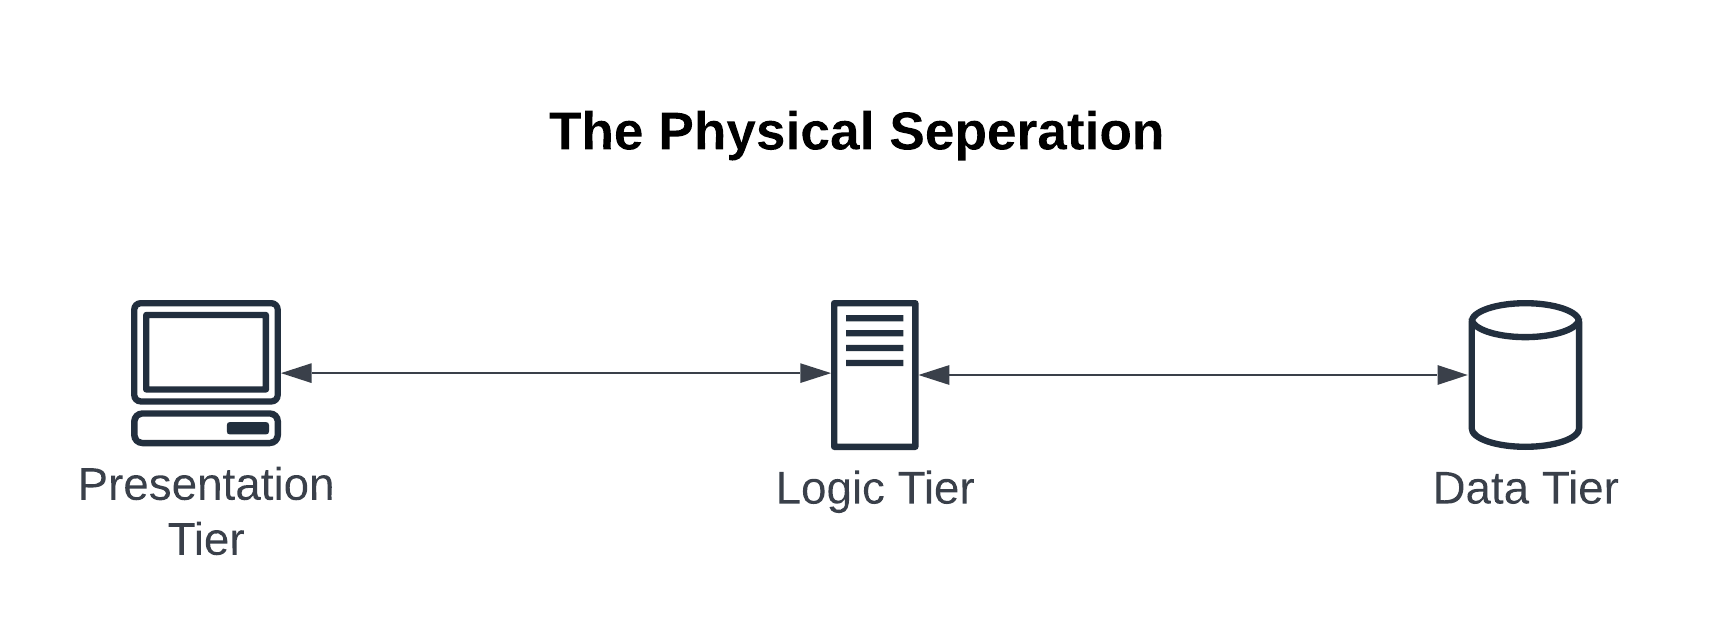
\includegraphics[width=100mm,scale=1]{figures/analysis_and_design/design/Physical Seperation V1.png}}
    \caption{Physical separation}
    \label{physicalSeparation}
\end{figure}

\newendline {\textit{Logical Architecture}}\\
This is the logical separation of the application. Meaning logically where the application components are. The application has a Client (Frontend) and a Server (Backend).
\begin{enumerate}[itemsep=-0.3cm]
    \item The Frontend: is responsible for presentation tier of the application. Uses different technologies to illustrate user interface.
    \item The Backend: is responsible for logic tier and database tier of the application. Application logic and data access logic are all here.
\end{enumerate}

\vspace{0.25cm}
\newendline {\textit{Software Design Pattern}}\\
This is the software design pattern, meaning how the application is developed (is coded), this has nothing to do with physical design or logical design. MVC Design Pattern is used.
\begin{enumerate}[itemsep=-0.3cm]
    \item Model: is responsible for business logic, and model classes are here.
    \item Controller: is responsible for connecting the bridge between the model and the view. It receives user input.
    \item View: is responsible for representing the application user interface.
\end{enumerate}

\vspace{0.25cm}
\newendline {\textit{Implementation Paradigms}}\\
This is the approach used to code each component of the logical architecture. Two approaches are used here:
\begin{enumerate}[itemsep=-0.3cm]
    \item Object Orient Programming: is used for the backend of the application
    \item Functional Programming: is used for the frontend of the application.
\end{enumerate}

\vspace{0.25cm}
\newendline \textbf{\textit{Physical Architecture Design}}\\
The physical separation of concerns for the system physically, meaning this separation is machine separation. The machines used as mentioned before will be into 3 tiers. Below here each tier is explained.
\begin{enumerate}[itemsep=-0.15cm]
    \item Presentation Tier\\The presentation tier is responsible for showing the user interface of the application to the user. It runs separately from the other layers on clients’ machine. The presentation tier is also responsible for communicating with the logic tier.
    \item Logic Tier\\Processing data, carrying out calculations, and making logical decisions are the tasks that are within the scope of the logic tier. Because practically all of the system's business logic is maintained in this tier, it is sometimes referred to as the "heart" of the application. This tier is deployed onto a dedicated server as its machine that is available at all times.
    \item Data Tier\\This tier is responsible for handling the system’s data. A software that manages read and write access to a database is included inside the data tier or database tier of the system. This tier, which is also known to as a storage tier is hosted on a database server, a different machine from the other tiers.
\end{enumerate}

\vspace{0.25cm}
\noindent In a three-tiered system, the logic tier is the point at which all interaction is routed. Both the presentation tier and the database tier are separated from each other and are unable to connect to each other explicitly.

\begin{figure}[H]
    \centerline{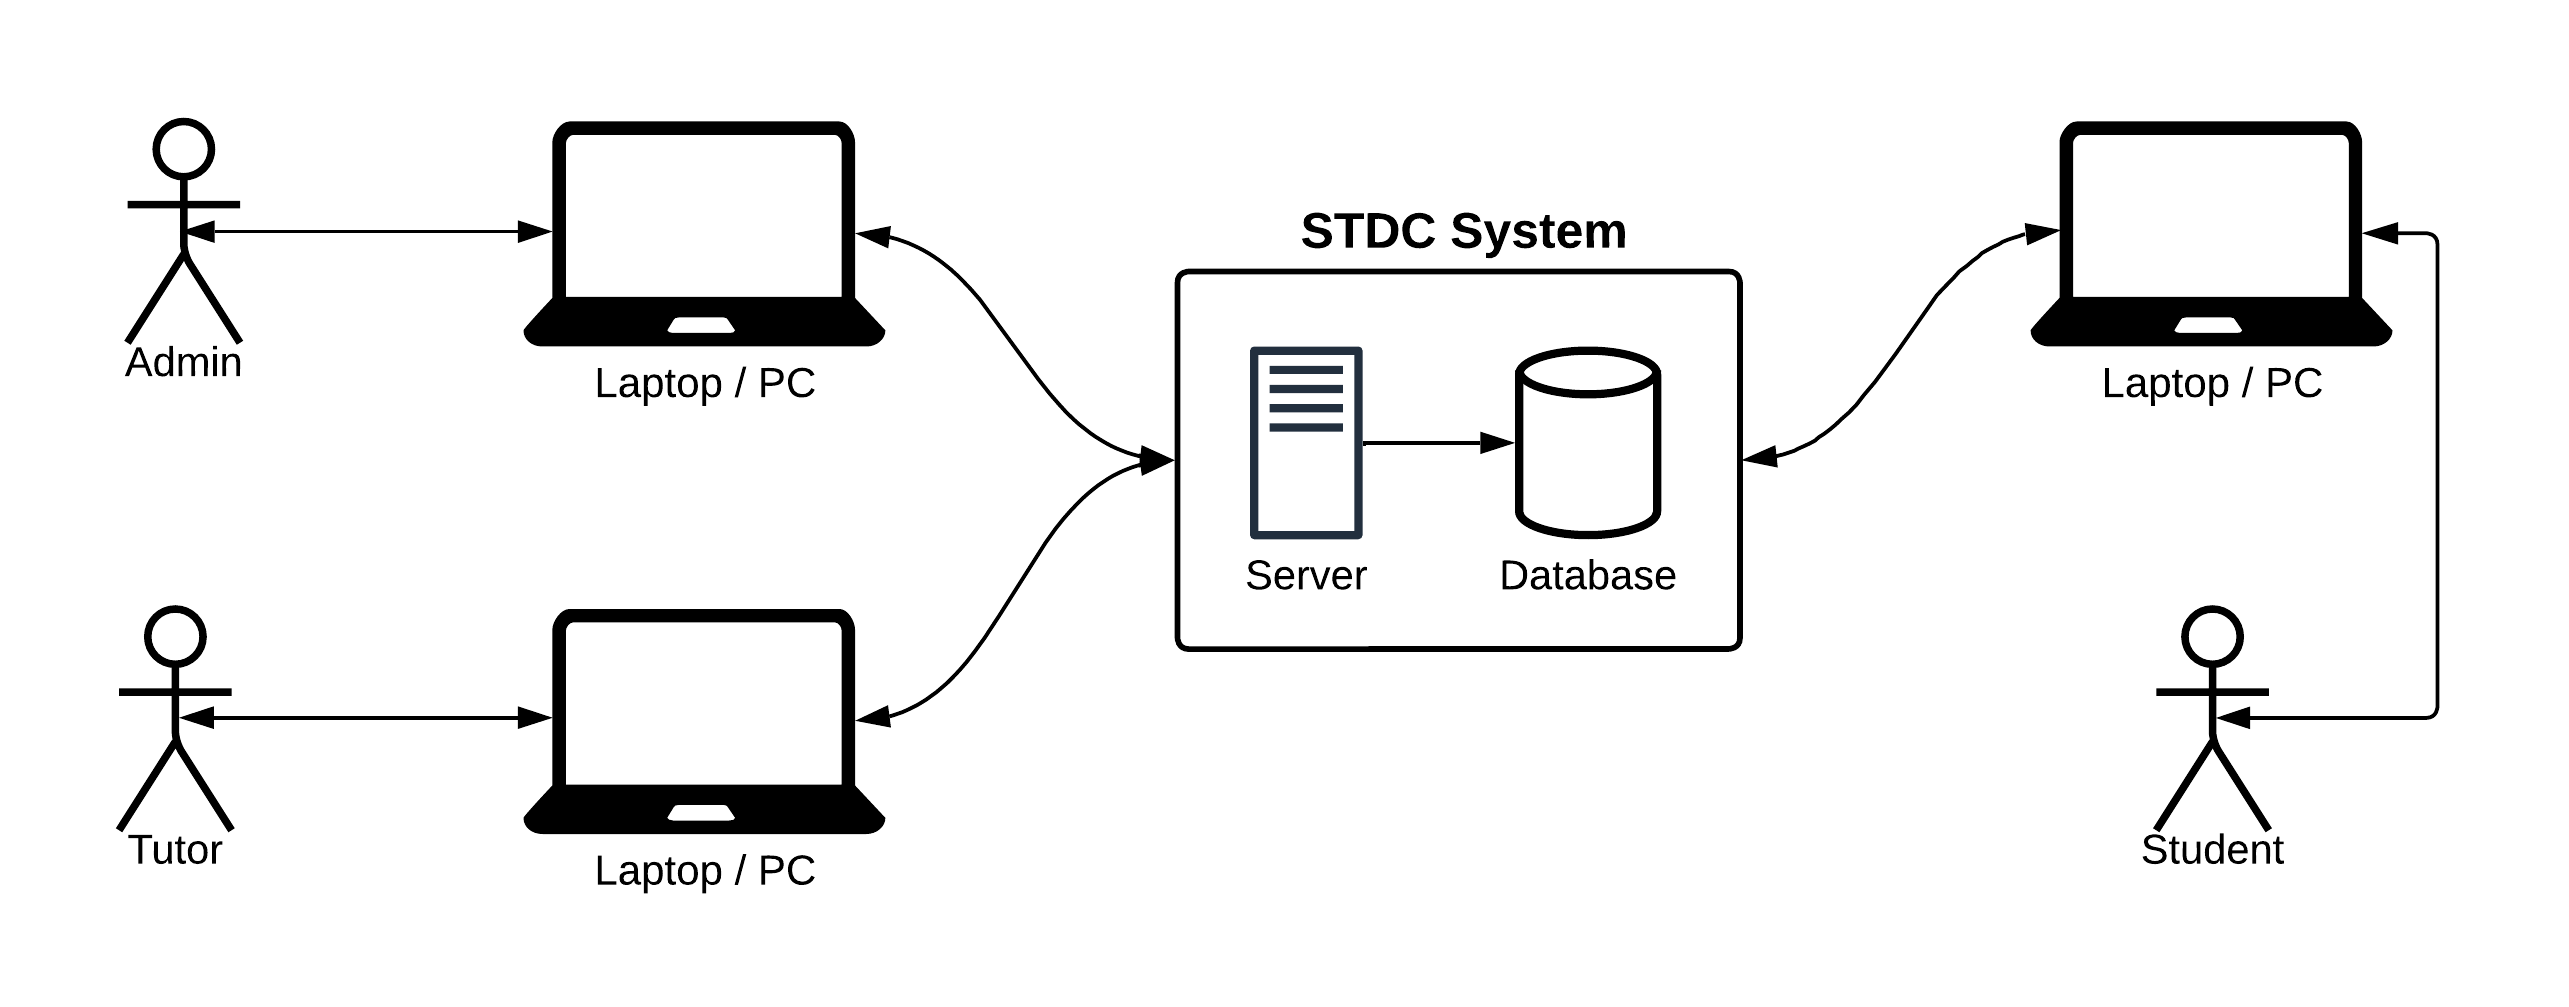
\includegraphics[width=150mm,scale=1]{figures/analysis_and_design/design/User Interaction V1.png}}
    \caption{User interaction}
    \label{UserInteraction}
\end{figure}

\newendline \textbf{\textit{Logical Architecture Design}}\\
The logical design architecture is extremely straightforward and basic. It consists of a client, also known as the frontend, submitting a request to the server, also known as the backend, in in order to receive a response from the server. The request coming from the client may be any one of post, get, put, delete, or patch, but it would still need to include an authorization parameter in the header. This authorization parameter would include the user's access token that was acquired from the identity server. The client's request is then dealt with by the server, and the results are sent back to the client in JSON format. Take note that the server will interact with the database in the event that this becomes necessary. Below here the pattern of development of each the client (frontend) and the server (backend) will be discussed in further details.

\begin{figure}[H]
    \centerline{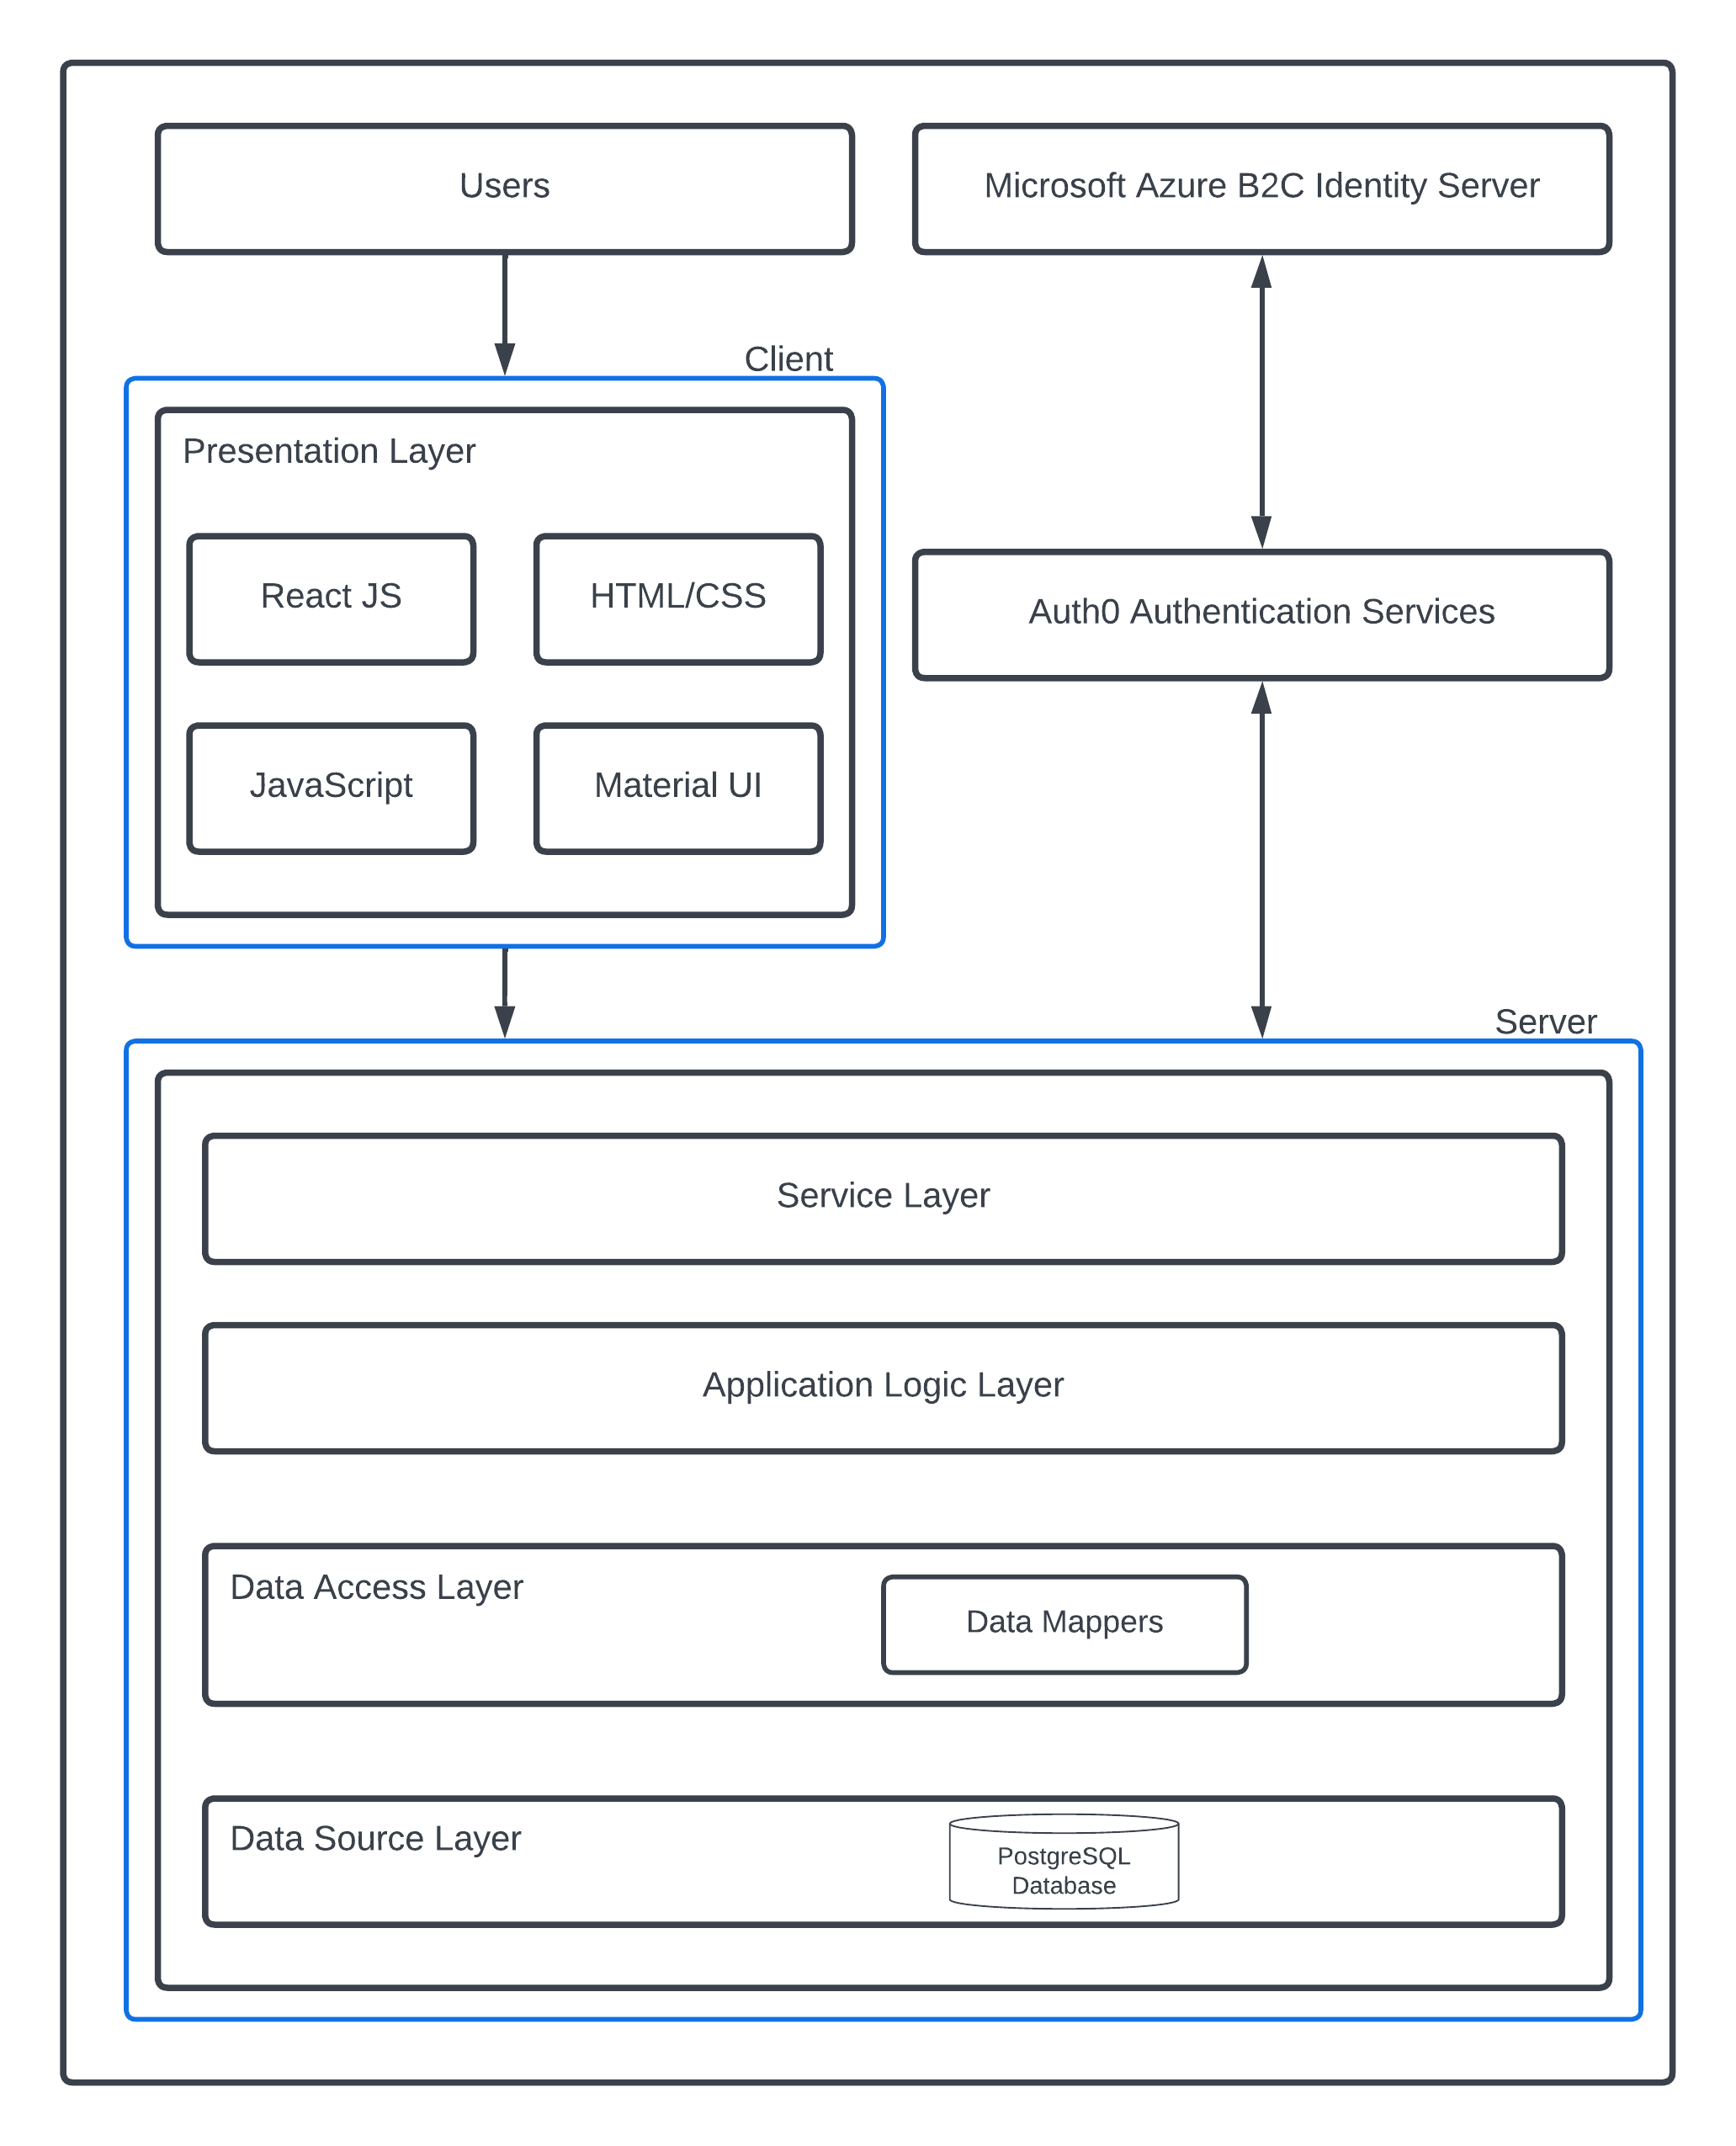
\includegraphics[width=150mm,scale=1]{figures/analysis_and_design/design/Logical Layer V2.png}}
    \caption{Logical layer}
    \label{LogicalLayer}
\end{figure}

\newendline \textbf{\textit{Software Design Pattern}}\\
The student talent development center web application will be developed using the MVC design pattern.

\vspace{0.25cm}
\newendline {\textit{Model-View-Controller (MVC)}}\\
It is a design pattern is a software architecture pattern that separates the representation of information from the user's interaction. This pattern divides the application into 3 main components: model, view, and controller.
\begin{enumerate}[itemsep=-0.3cm]
    \item The model represents data and business logic of the application, It is responsible for managing the data, validating user input, and performing any other business-related tasks. This component resides in the server (the backend).
    \item The view represents the user interface of the application. It is responsible for displaying the data to the user and providing a way for the user to interact with the application. This component resides in the client (the frontend).
    \item The controller is the bridge between the model and the view. It receives user input, communicates with the model to perform any necessary actions, and then updates the view with the results. This component resides in the server (the backend).
\end{enumerate}

\vspace{0.25cm}
\noindent The MVC design pattern helps to improve the separation of concerns in the application and makes it easier to maintain the different parts of the application independently.

\begin{figure}[H]
    \centerline{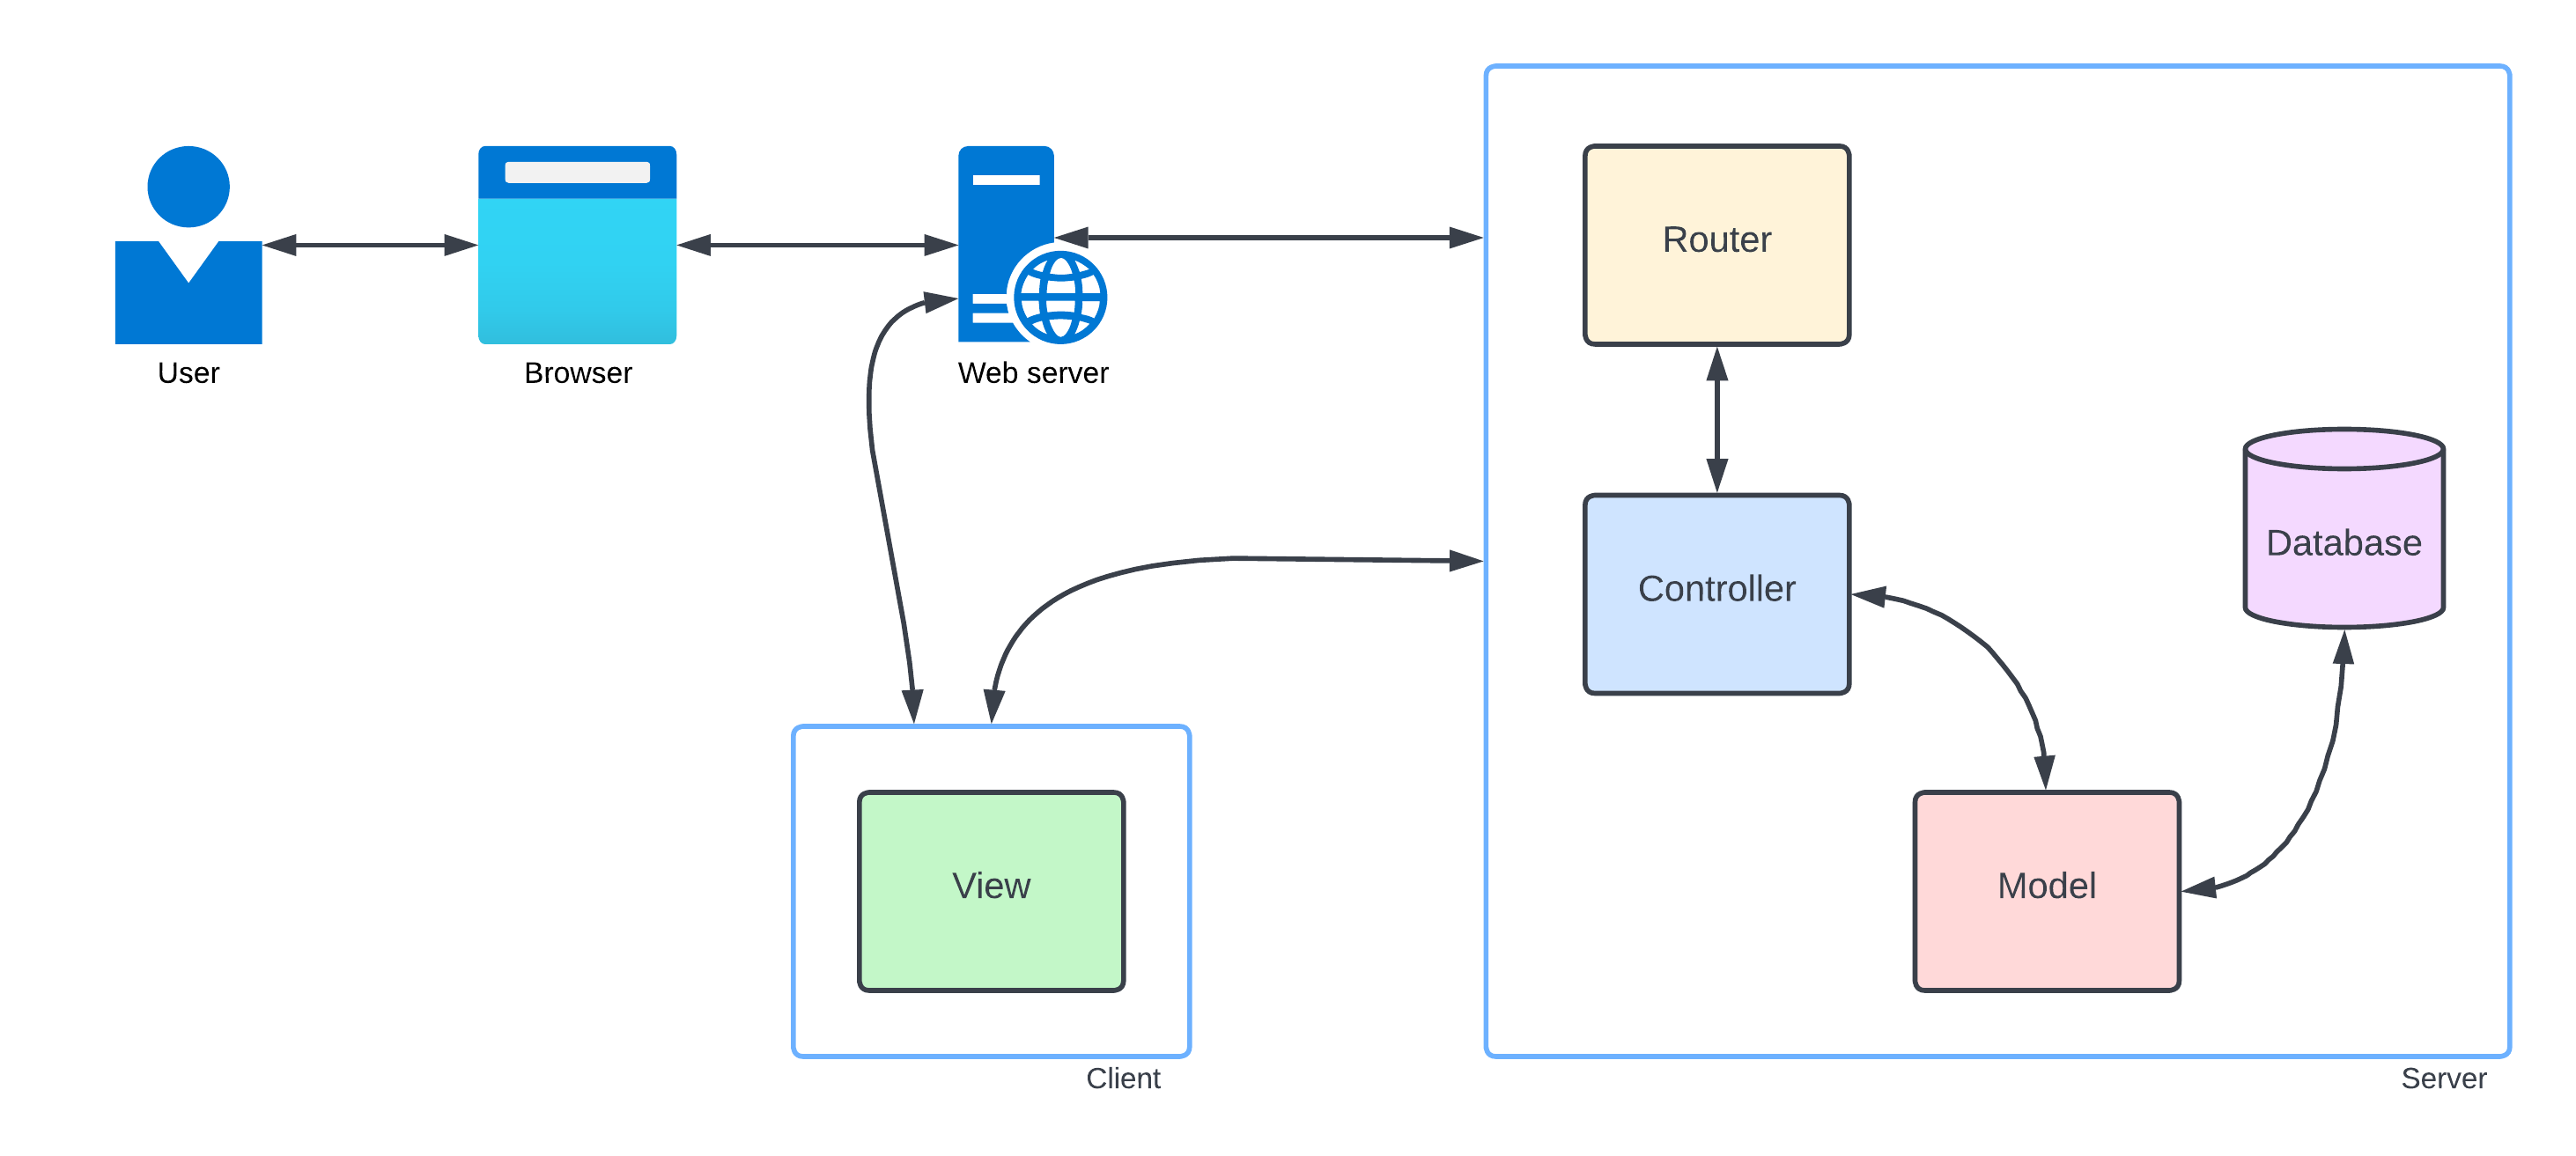
\includegraphics[width=150mm,scale=1]{figures/analysis_and_design/design/MVC V1.png}}
    \caption{MVC pattern}
    \label{MVC}
\end{figure}

\newendline \textbf{\textit{Implementation Paradigms}}\newendline
The student talent development center web application will be developed using two different programming paradigms. The backend will be developed using Ruby on Rails framework by implementing the Object-Oriented Programming concepts. The frontend will be developed using React JS framework by implementing the Functional Programming concepts. Functional programming and object-oriented programming (OOP) are two programming paradigms, or approaches to writing software.

\vspace{0.25cm}
\newendline The evaluation of mathematical functions is the basis for computing in the functional programming paradigm. It is based on the idea of using functions to model computation, and it is characterized by the use of immutable data, higher-order functions, and a focus on pure functions. In functional programming, functions are first-class citizens, which means that they can be passed as arguments to other functions and returned as values from functions.

\vspace{0.25cm}
\newendline Object-oriented programming is a programming paradigm which is based on the concept of "objects," which represent data and the functions that operate on that data. In OOP, objects are created from templates called classes, and they can interact with each other through methods. OOP is characterized by the use of encapsulation, inheritance, and polymorphism.

\vspace{0.25cm}
\newendline Both functional programming and OOP have their own strengths and can be useful in different contexts. Therefore, both of them are chosen to be used in combination to one another.
\end{justify}
\clearpage
\subsection{Program Design}
\begin{justify}
    The following is the Program Design of the Student Talent Development Center Web Application. First, attention is given to the class modelling that consist of both dynamic classes and static classes. Then the relationship between classes is highlighted. After that, design pattern for each class is chosen. Lastly sequence models are illustrated to further explain the workflow of some of the complex areas of the application that have not been highlighted in the Use Case tables.

\vspace{0.25cm}
\newendline \textbf{\textit{Class Model (Class Diagram)}}\newendline
The following class diagram contains both dynamic and the static classes. The Controller classes have a direct association with their corresponding classes (which are model classes). It has not been shown the diagram below for it will make the diagram very complex, however direct association exist between those controllers and model classes.

\begin{figure}[H]
    \centerline{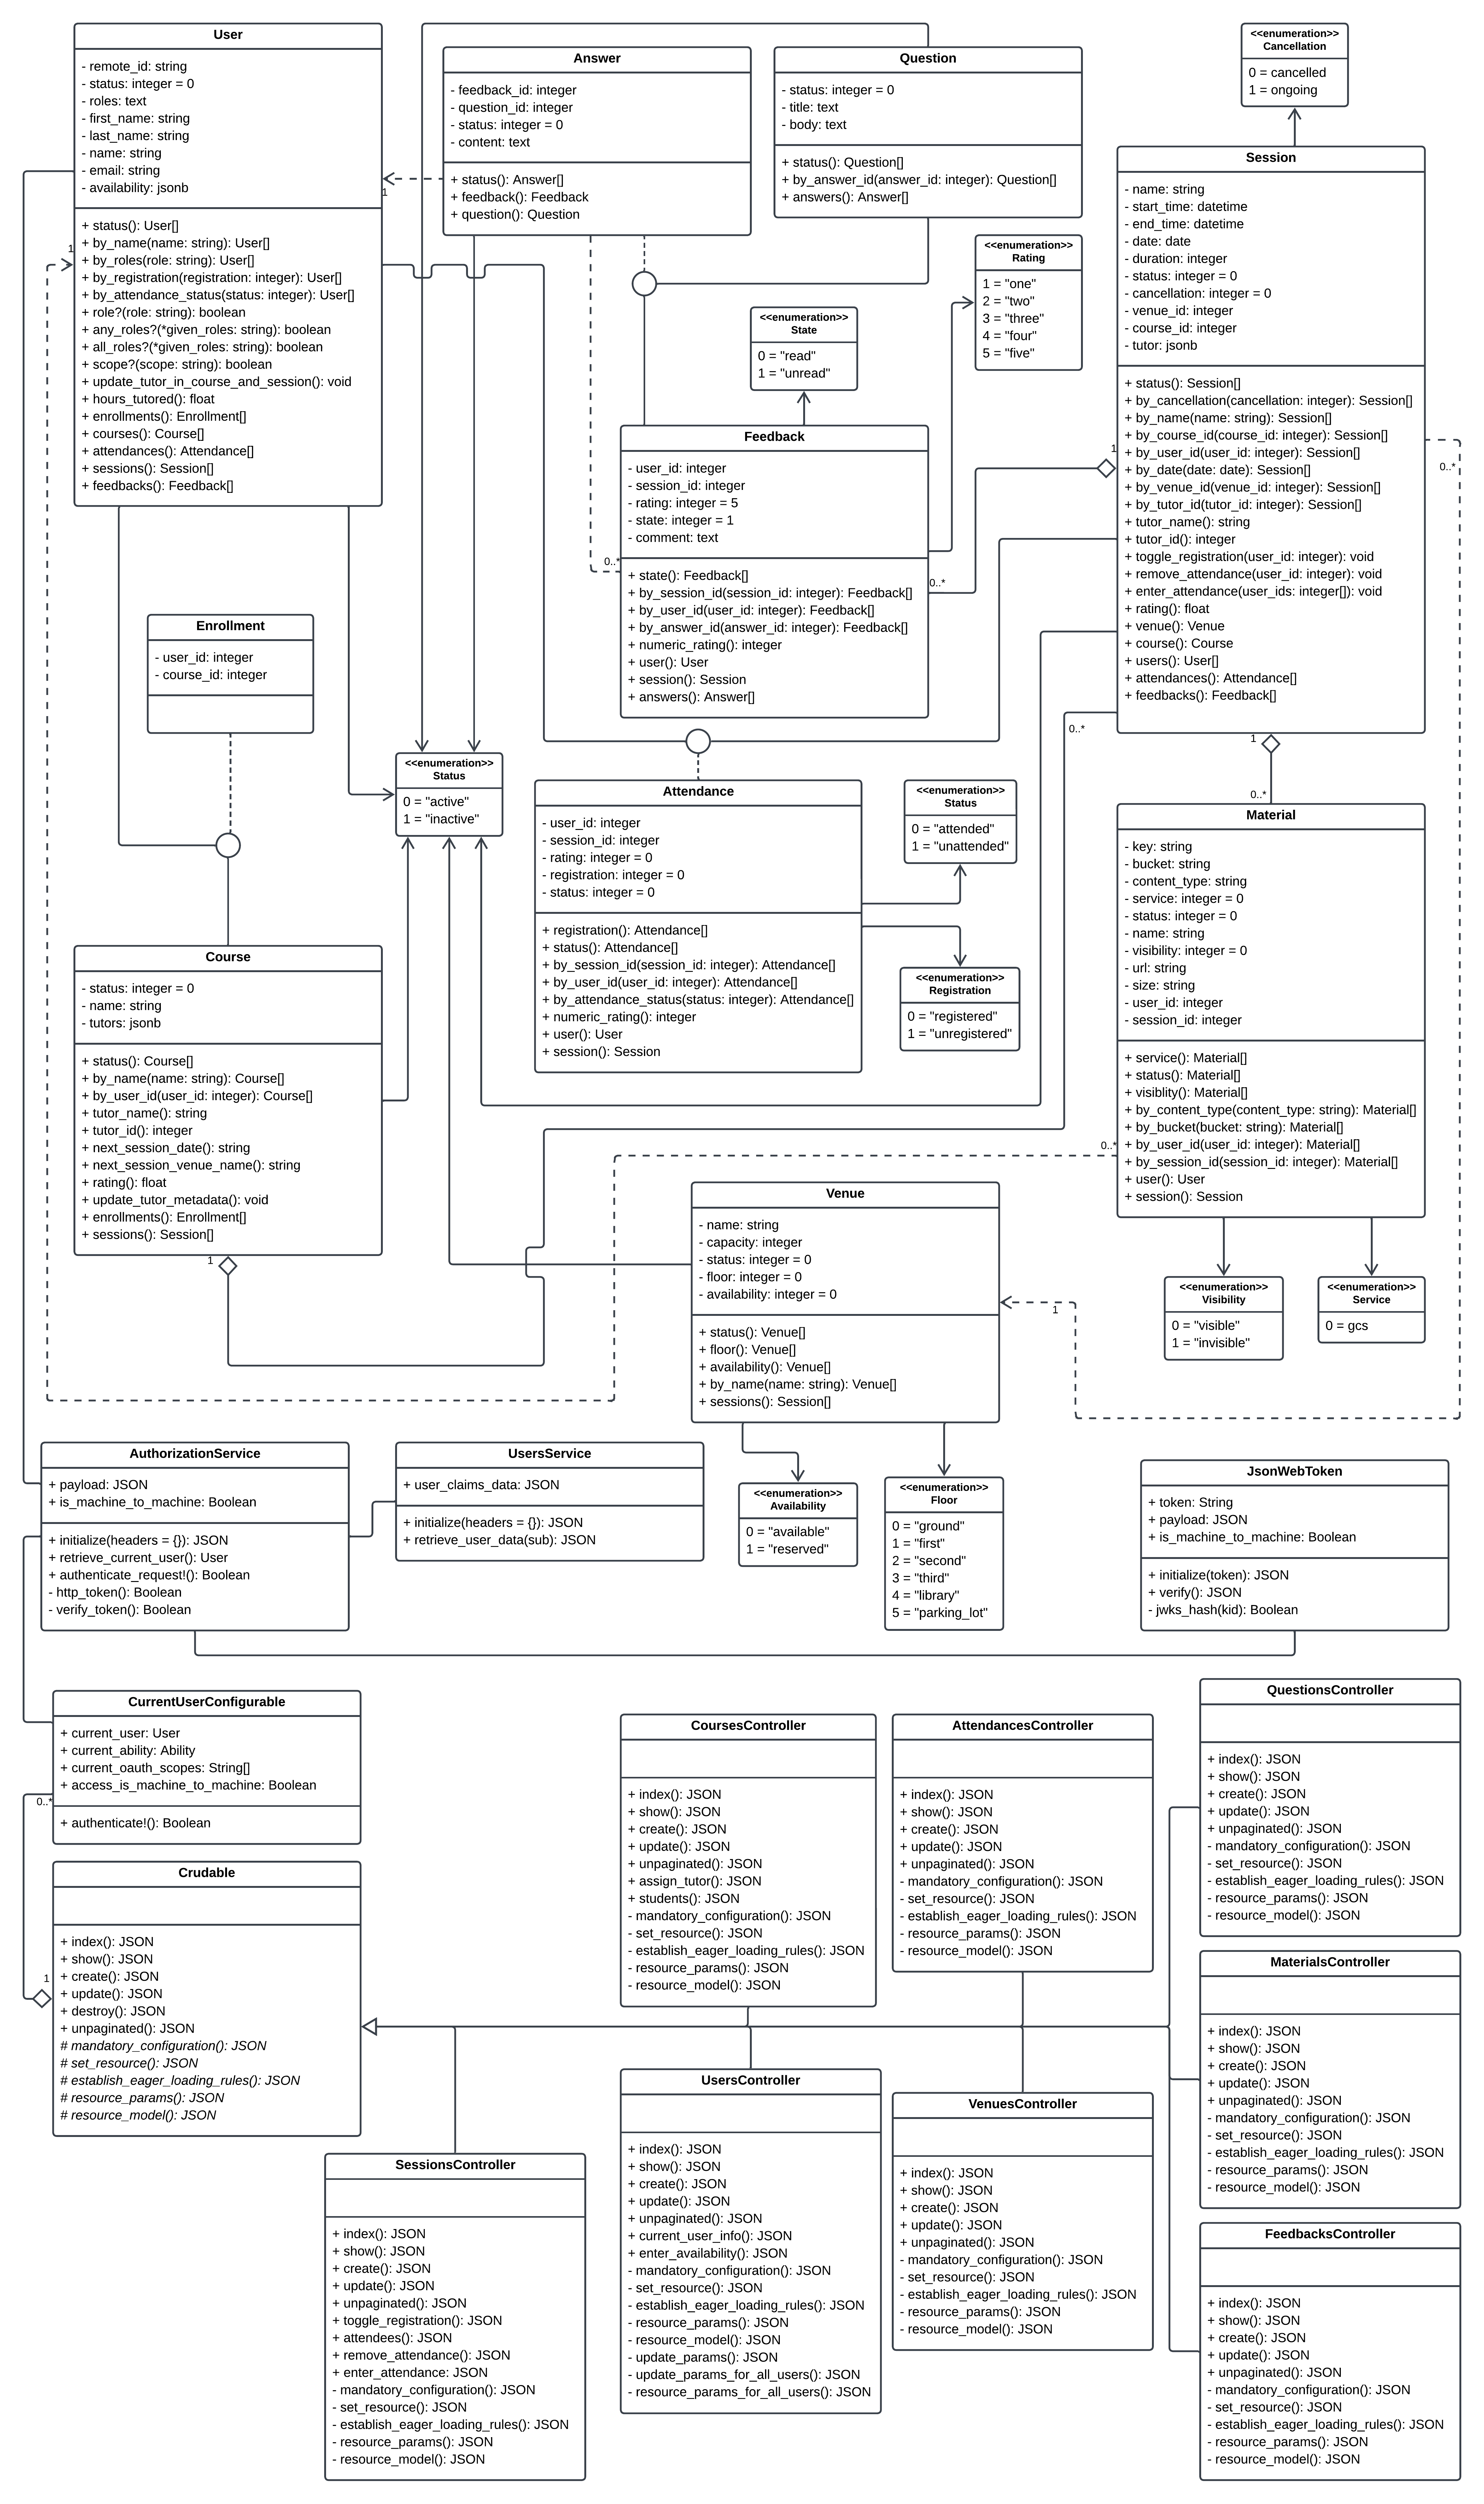
\includegraphics[width=140mm,scale=1]{figures/analysis_and_design/design/Dynamic Class Diagram V3.png}}
    \caption{Class model -- dynamic and static classes}
    \label{ClassModelStaticAndDynamic}
\end{figure}

\begin{figure}[H]
    \centerline{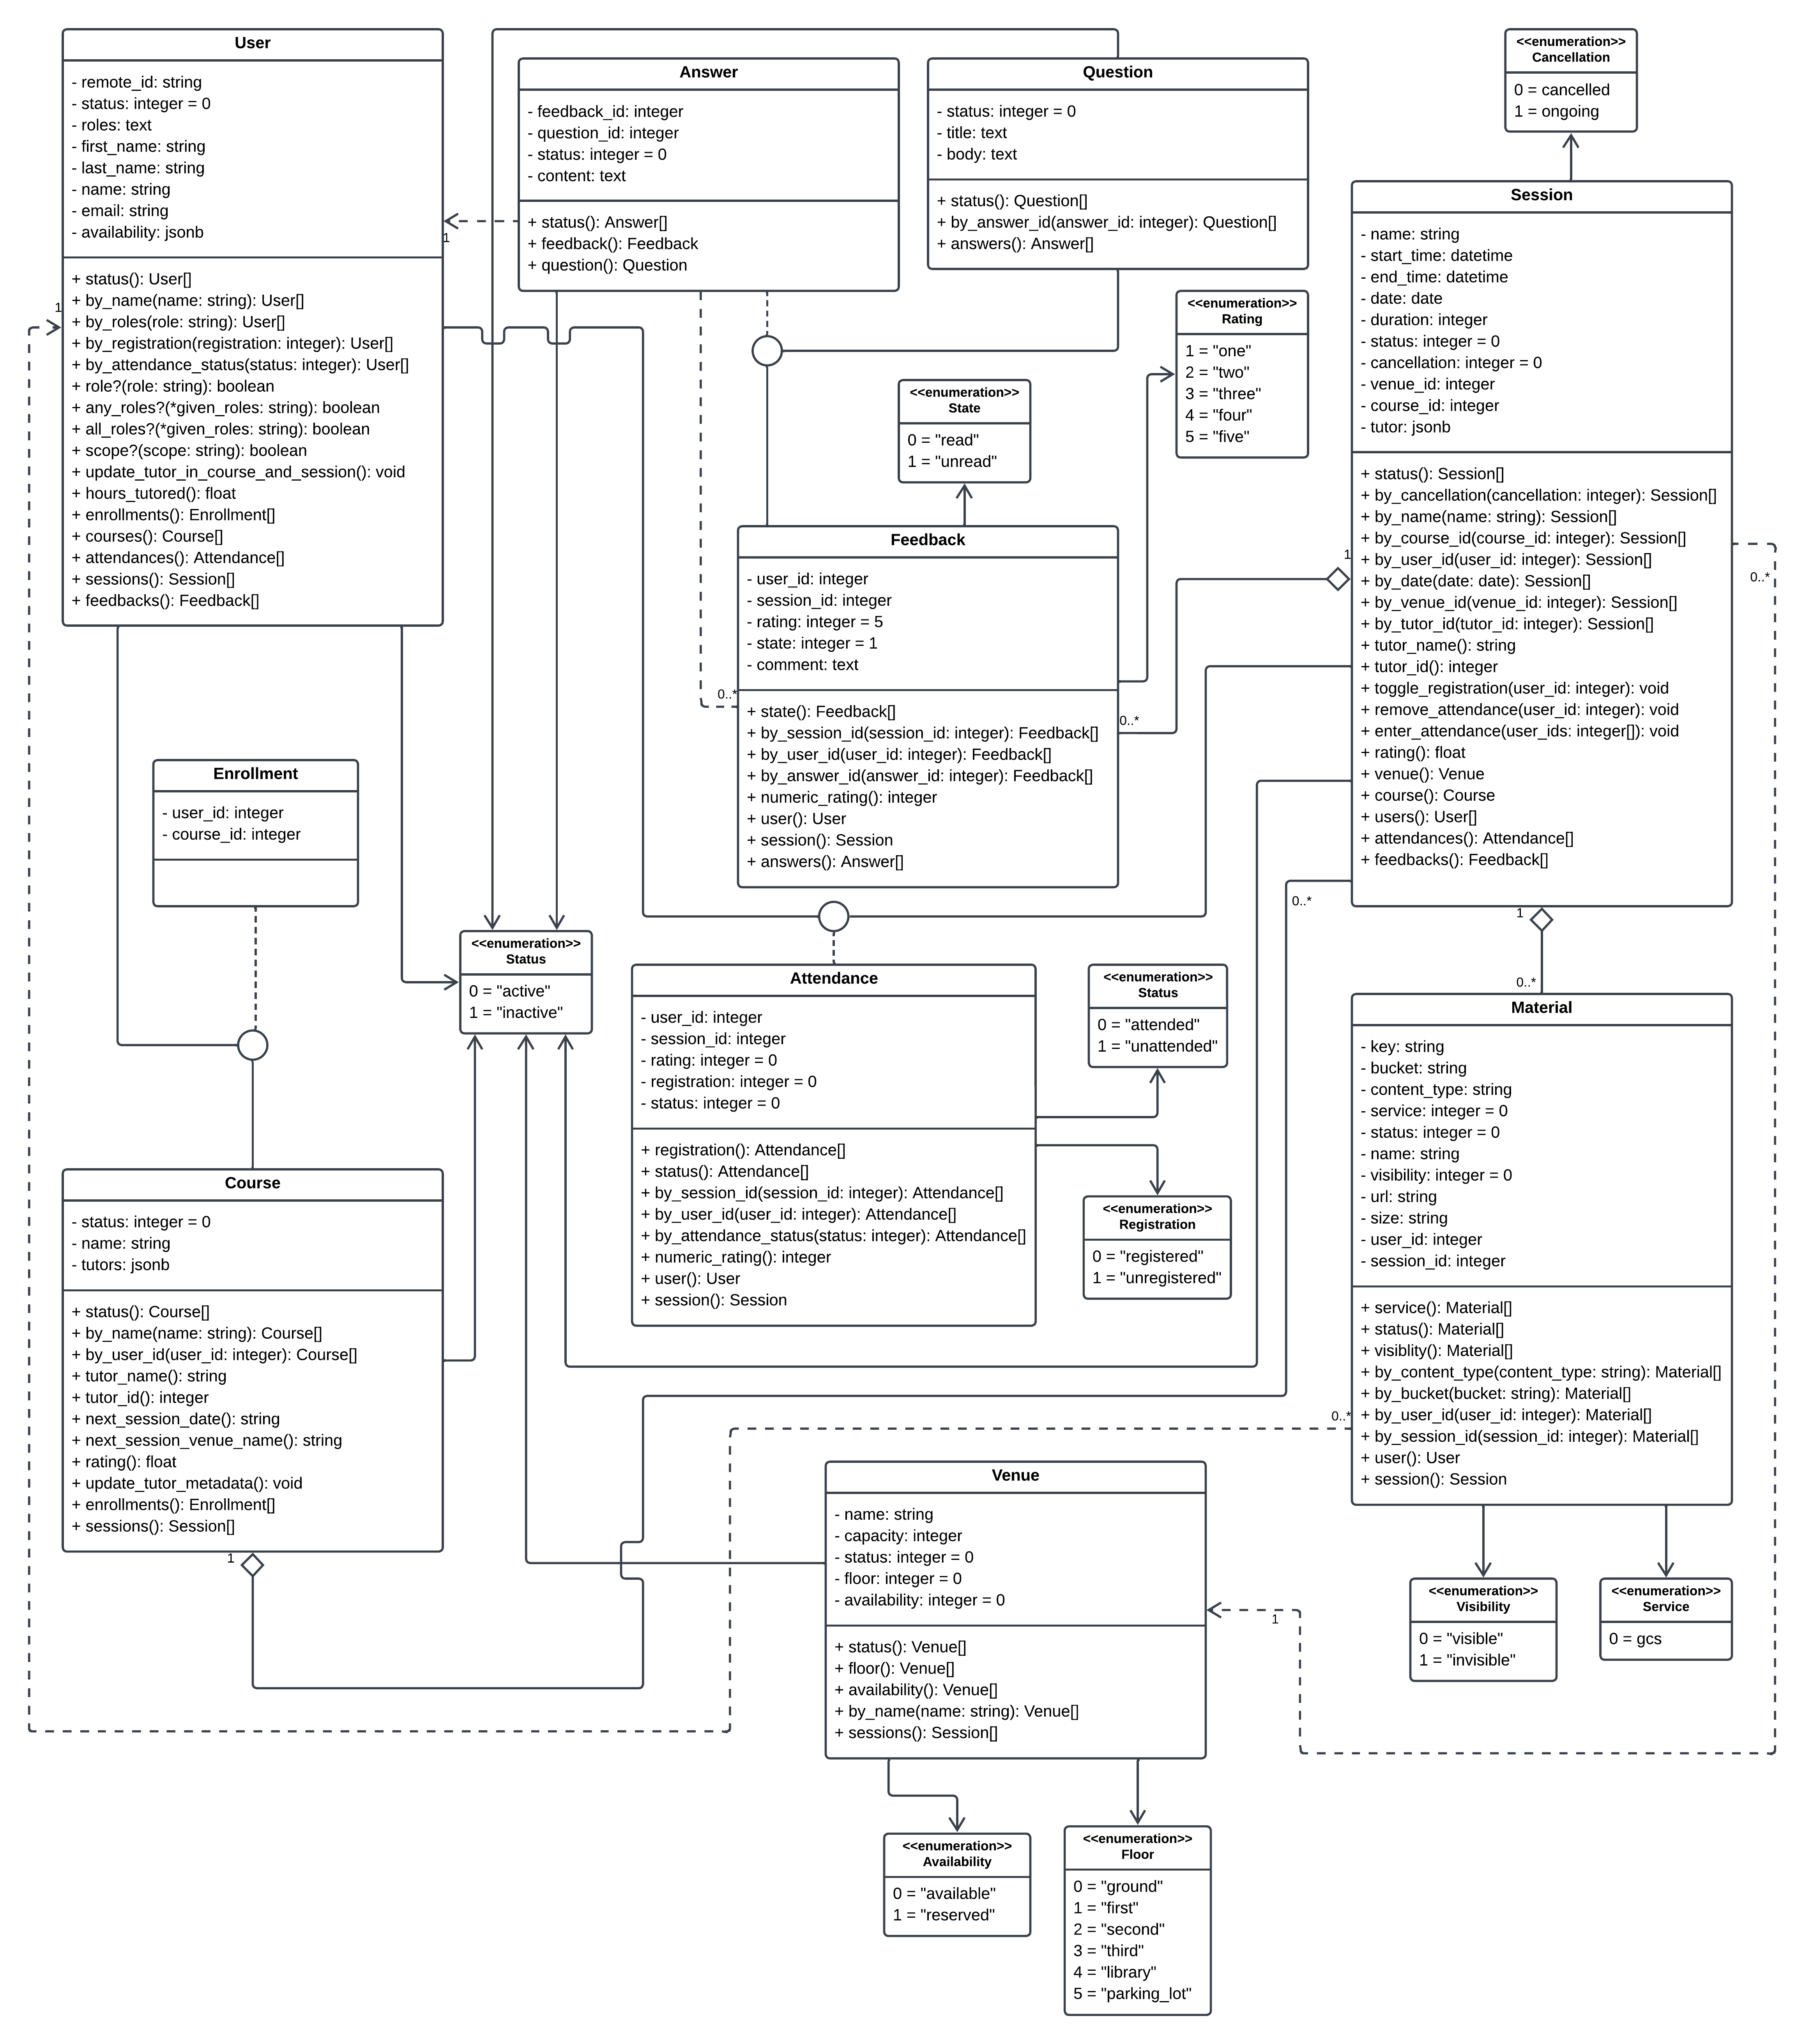
\includegraphics[width=140mm,scale=1]{figures/analysis_and_design/design/Static Class Diagram V3.png}}
    \caption{Class model -- static classes}
    \label{ClassModelStatic}
\end{figure}

\clearpage
\newendline \textbf{\textit{Class Design Pattern}}\newendline
The following is the chosen design pattern for each class in the class diagram. A design pattern is a general repeatable solution to a commonly occurring problem in software design. A design pattern isn't a finished design that can be transformed directly into code. It is a description or template for how to solve a problem that can be used in many different situations.

\renewcommand{\arraystretch}{1.0}
\begin{table}[H]
\centering
\caption{Class design patterns}
\begin{tabular}{|p{7.25cm}|p{7.25cm}|} 
\hline
\rowcolor[rgb]{0.835,0.863,0.894} \textbf{Class Name} & \textbf{Design Pattern}  \\ 
\hline
User                                                  & Active Record            \\ 
\hline
Course                                                & Active Record            \\ 
\hline
Enrollment                                          & Structural Pattern       \\ 
\hline
Feedback                                              & Active Record            \\ 
\hline
Attendance                                            & Active Record            \\
\hline
Answer                                            & Active Record            \\ 
\hline
Question                                            & Active Record            \\ 
\hline
Venue                                                 & Active Record            \\ 
\hline
Material                                              & Active Record            \\ 
\hline
Session                                               & Active Record            \\ 
\hline
AuthorizationService                                  & Service                  \\ 
\hline
JsonWebToken                                          & Factory                  \\ 
\hline
CurrentUserConfigureable                              & Interactor               \\ 
\hline
UsersService                                          & Service                  \\ 
\hline
Crudable                               & Template Method                  \\ 
\hline
AttendancesController                                              & Front Controller          \\ 
\hline
UsersController                                       & Front Controller         \\ 
\hline
CoursesController                                     & Front Controller         \\ 
\hline
FeedbacksController                                   & Front Controller         \\ 
\hline
VenuesController                                      & Front Controller         \\ 
\hline
SessionsController                                    & Front Controller         \\ 
\hline
MaterialsController                                   & Front Controller         \\
\hline
\end{tabular}
\end{table}


\vspace{0.25cm}
\newendline \textbf{\textit{Sequence Model (Sequence Diagram)}}\newendline
The followings are two sequence models (diagrams), first explaining how a current user in the application is set, and the second is the role of identity provider in the application in action. The rest does not require a sequence diagram for they have been clearly explained using the use case tabular form. The steps there with its reference to the user interface makes the process clear and easy to understand.\newendline
The first sequence diagram is the identity provider in action and shows how a request is authenticated by verifying the public keys and the access token received. The second sequence diagram is to show the process of setting the current user (login alike process).

\begin{figure}[H]
    \centerline{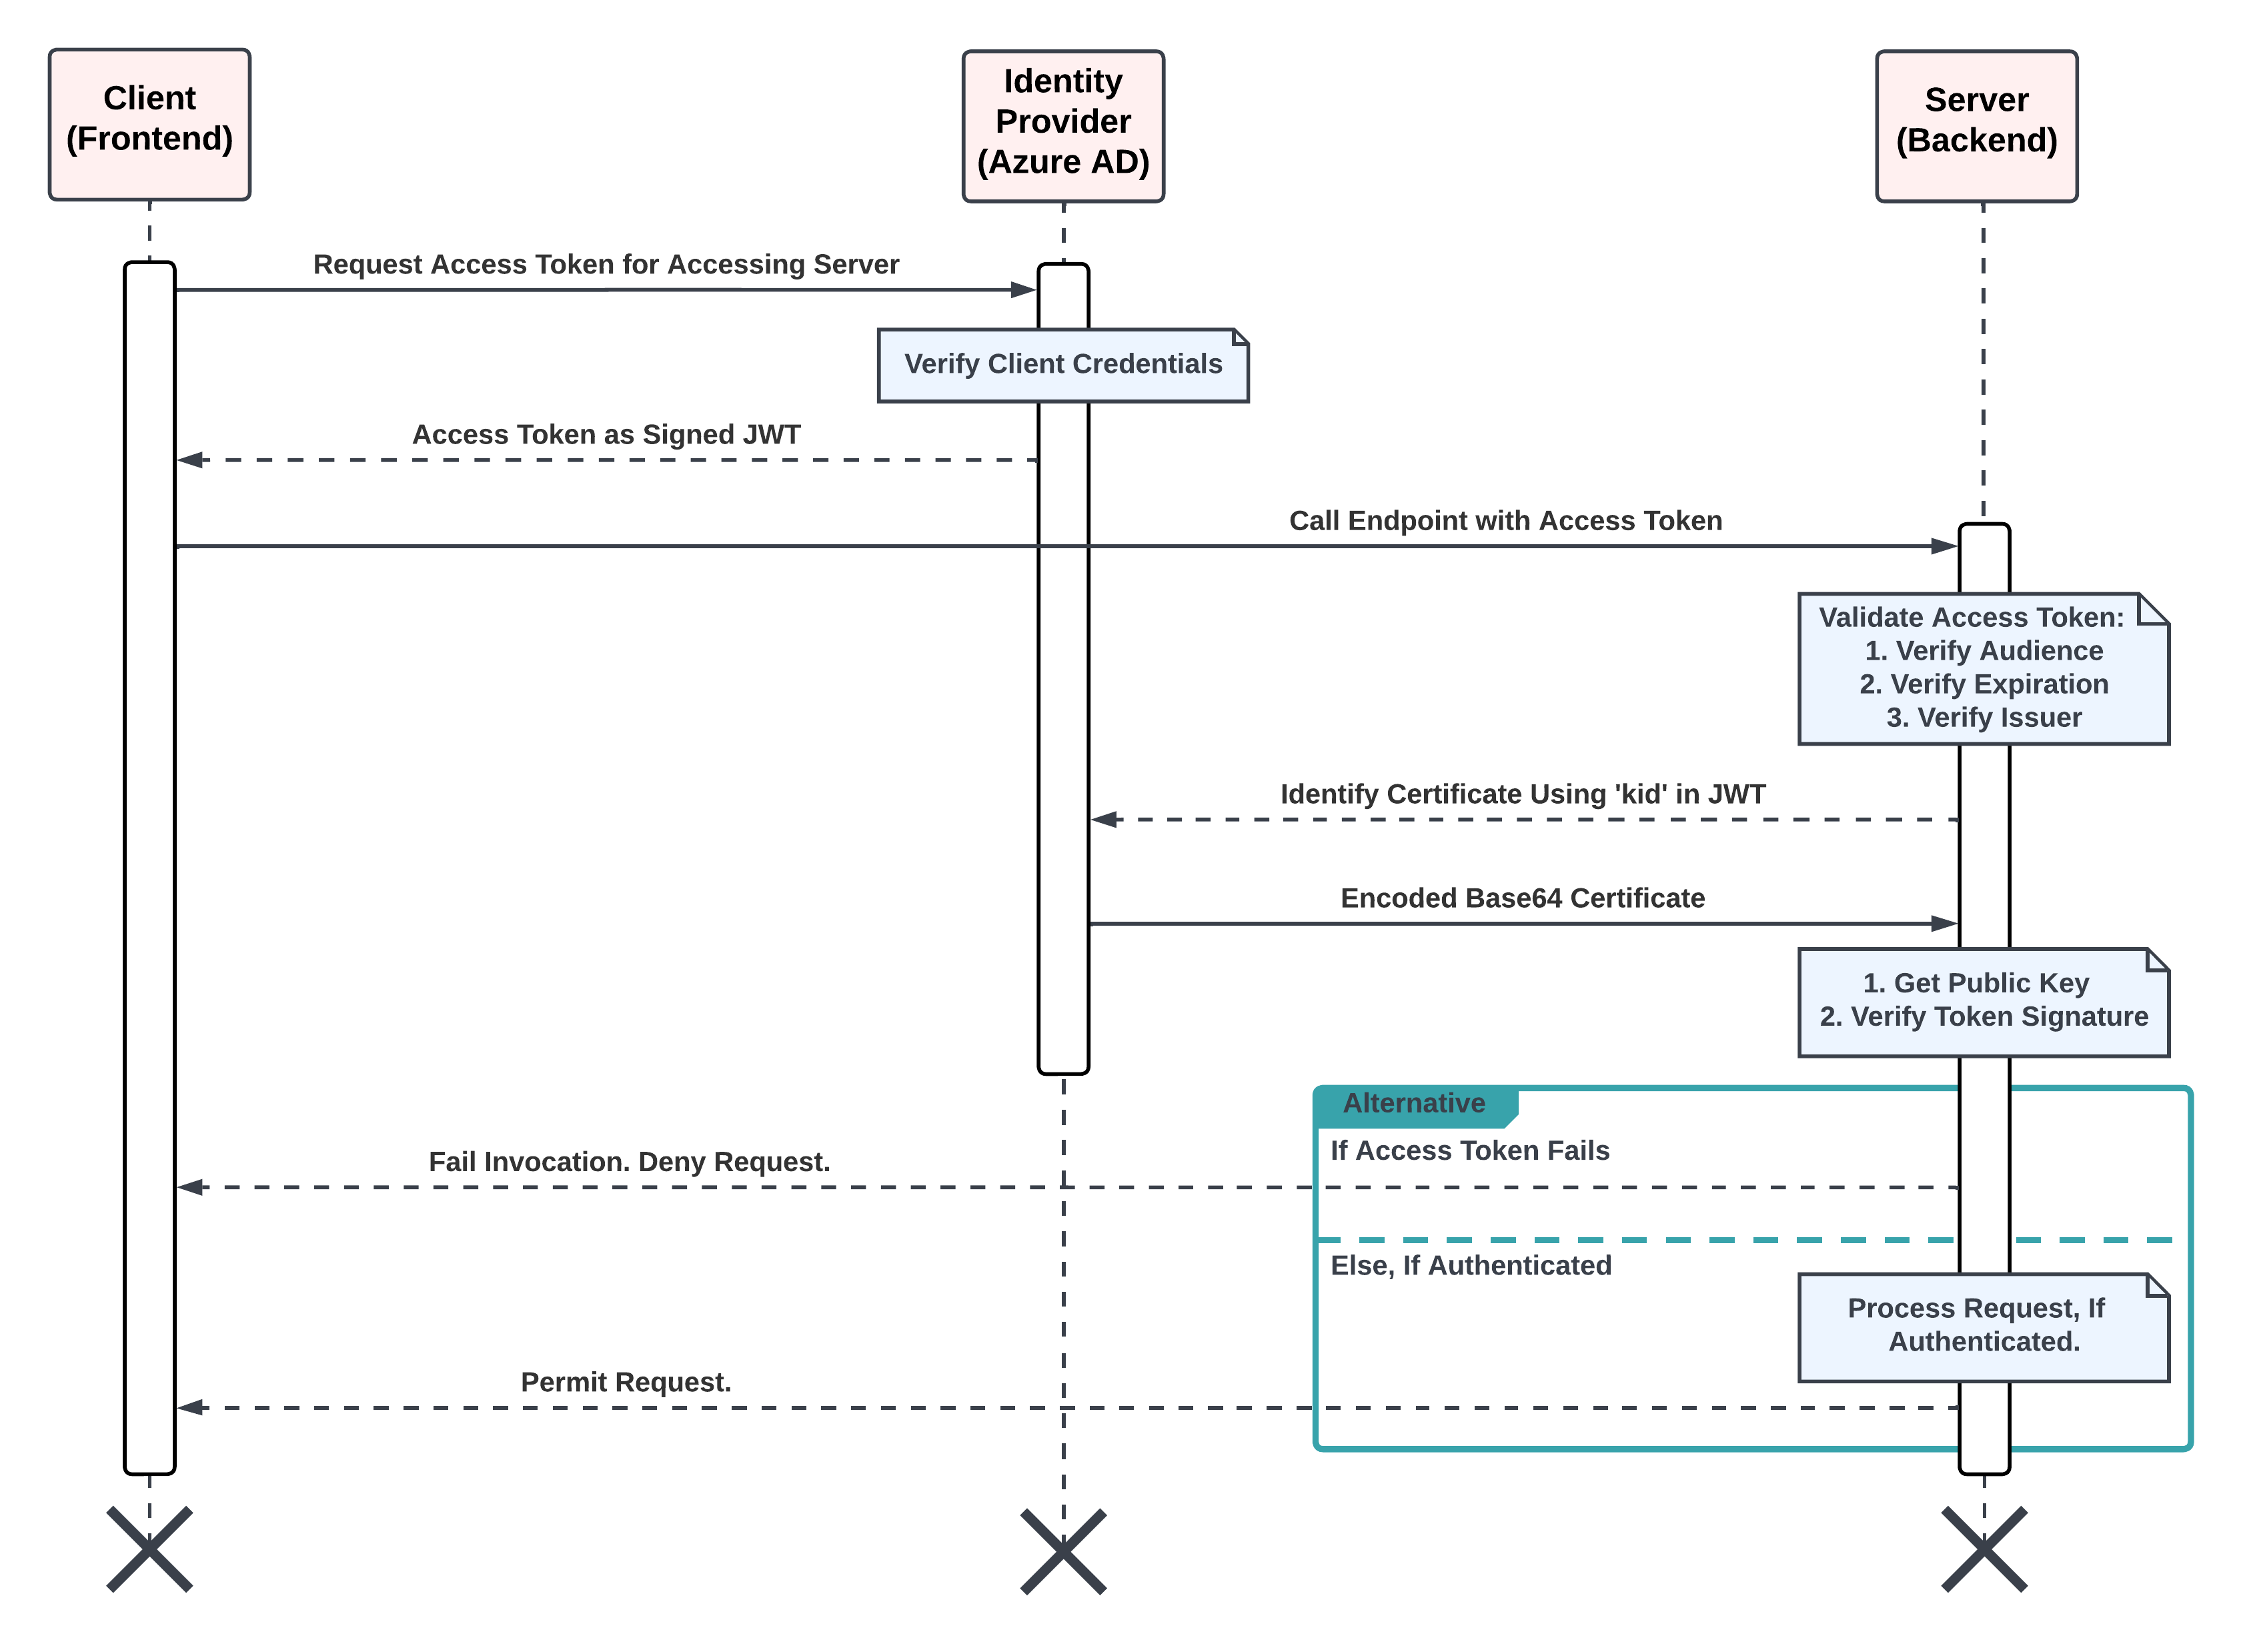
\includegraphics[width=150mm,scale=1]{figures/analysis_and_design/design/1. Identity Provider In Action.png}}
    \caption{Sequence model -- identity provider in action}
    \label{identityProvider}
\end{figure}

\begin{figure}[H]
    \centerline{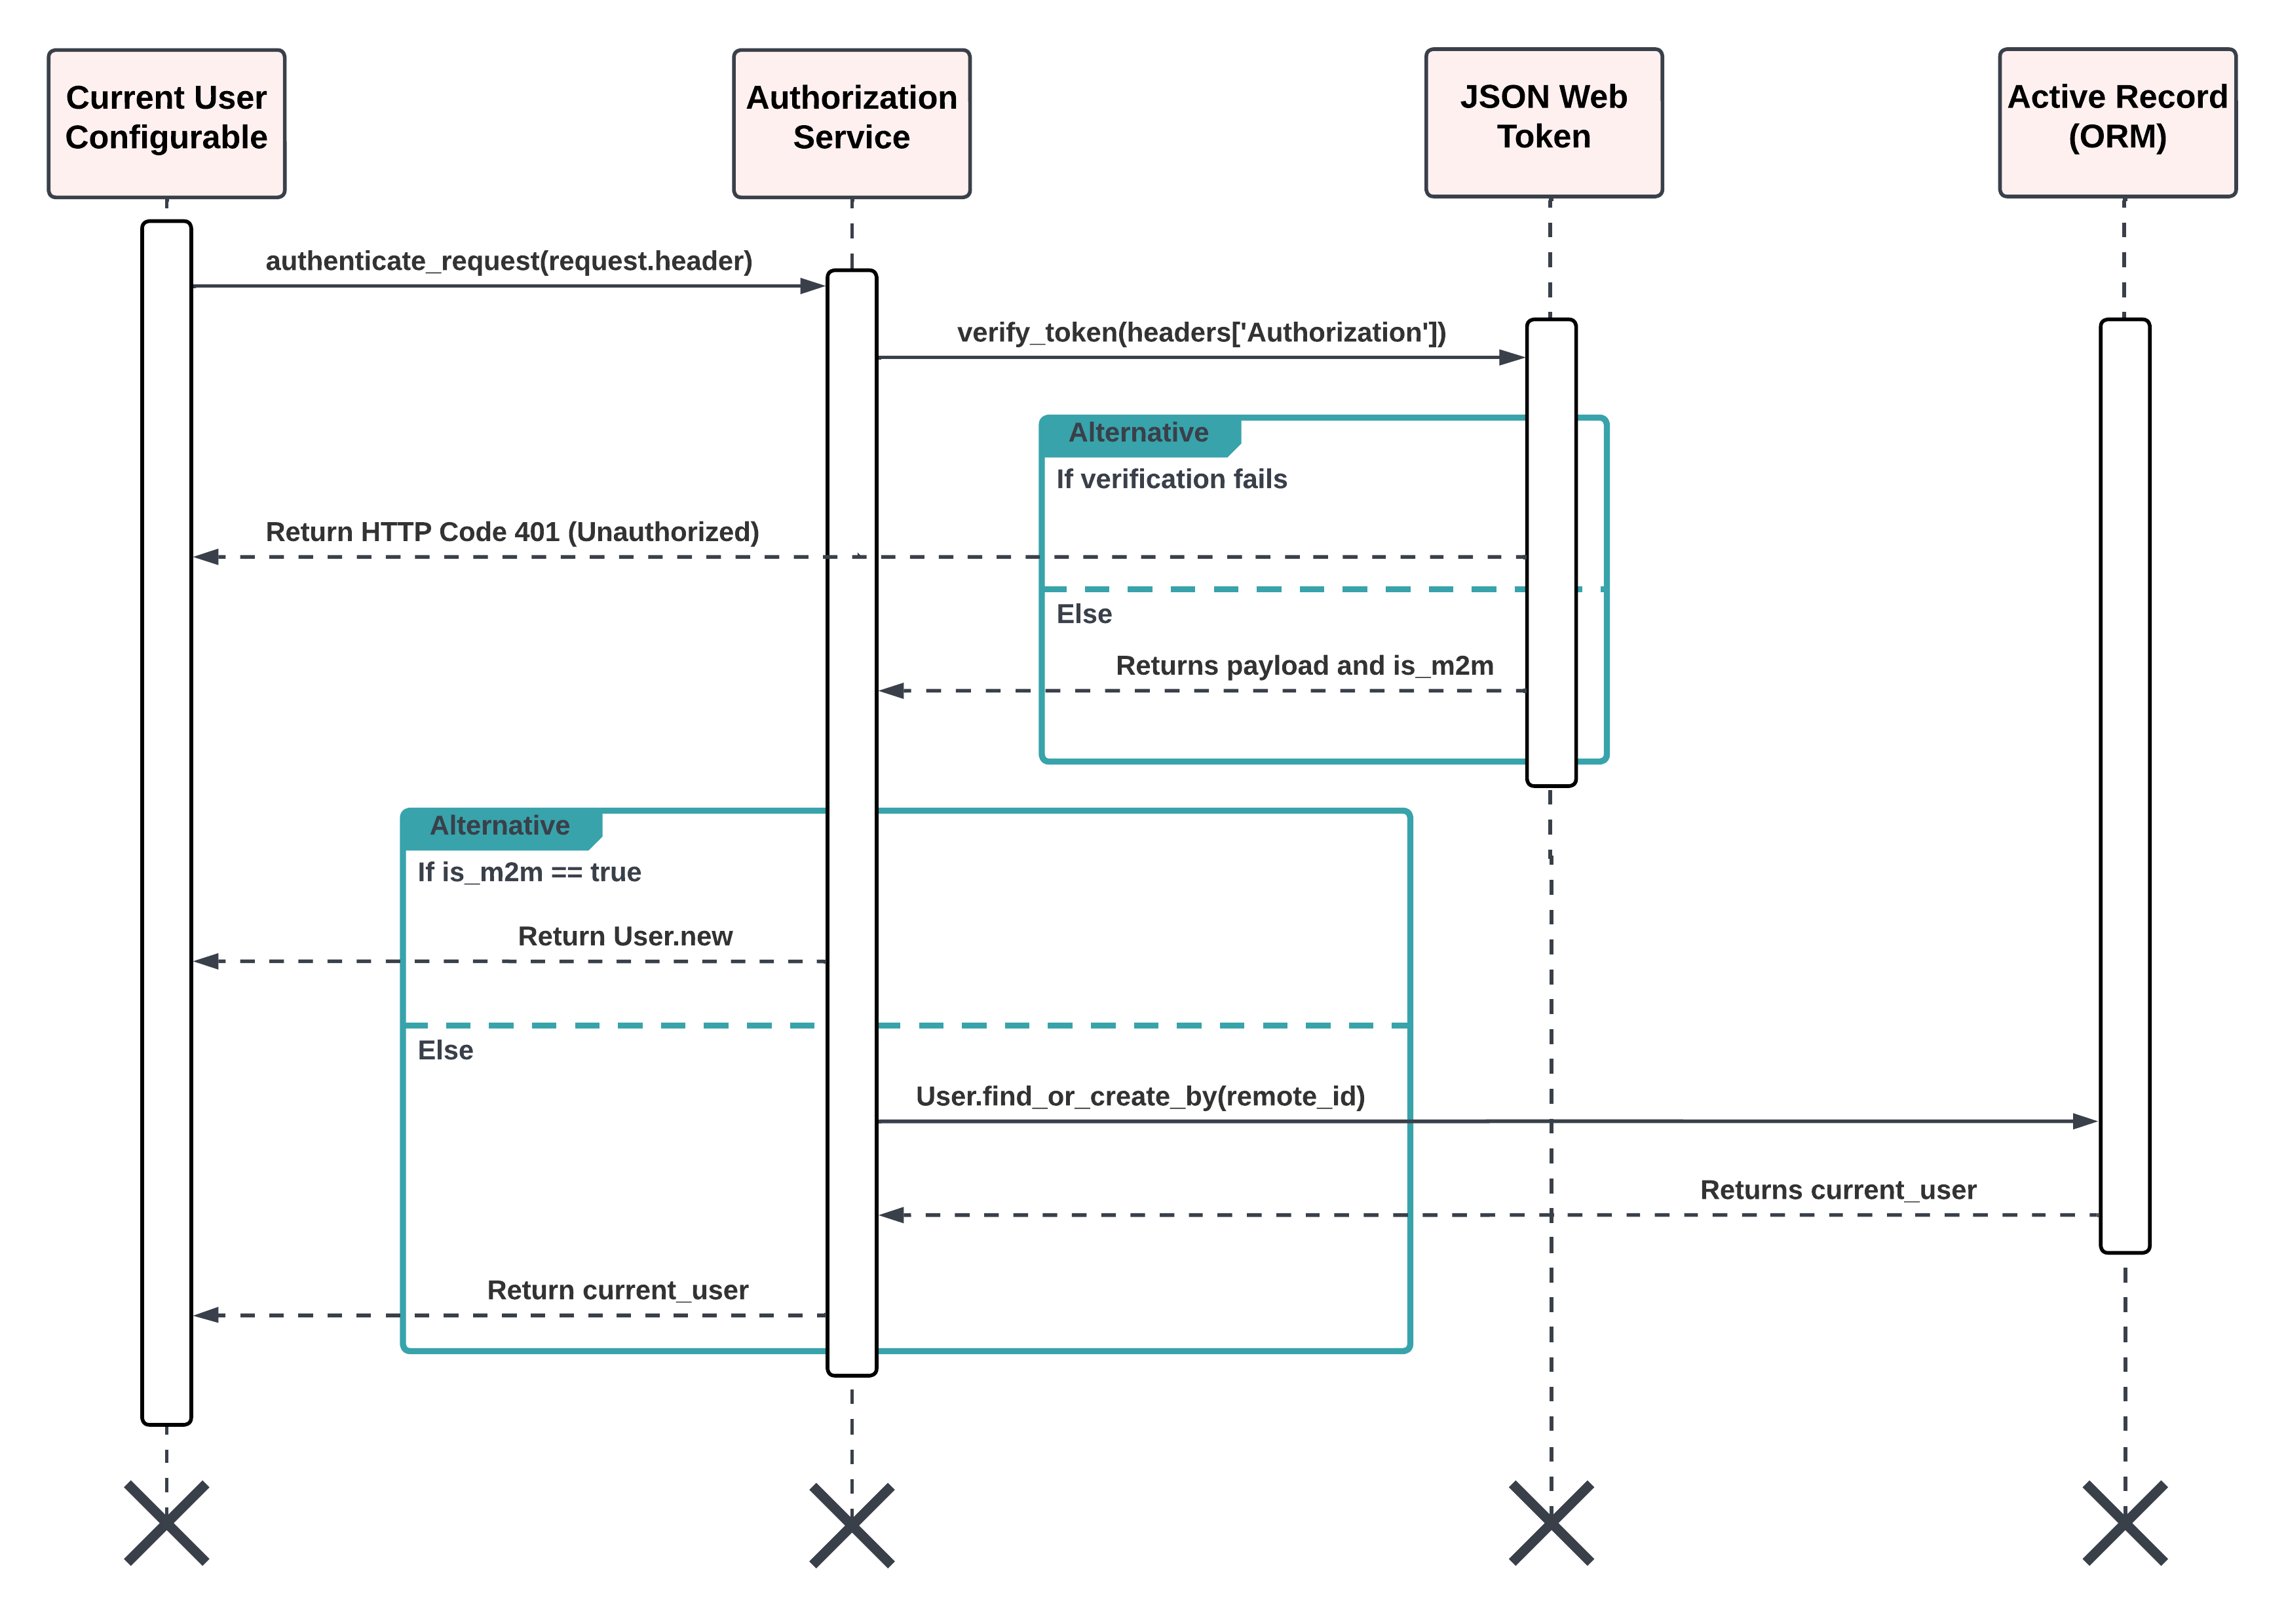
\includegraphics[width=150mm,scale=1]{figures/analysis_and_design/design/2. Set Current User.png}}
    \caption{Sequence model -- setting the current user}
    \label{settingCurrentUser}
\end{figure}
\end{justify}
\clearpage

\subsection{Interface Design}
\begin{justify}
    The following is the User Interface Design of the Student Talent Development Center Web Application. Though the application will end up having more specific user interfaces, below here the main pages of the application is illustrated along with landing page, and a form page that is used for creation, updating, or adding. The below user interfaces are created using FIGMA and there are few important assumptions that needs to be considered when viewing these user interfaces:

    \begin{enumerate}
        \item All the user interfaces are from the perspective of Admin. Except for “Profile” which is from the perspective of tutor.
        \item Each user interface has an associated id that is used for referencing purposes.
        \item When these user interfaces are viewed as student or tutor, they will be same except for the components that are not authorized for them to see. In that case, components are simply hidden away from the user without them noticing anything, this includes pages as well (e.g., Venues Page)
        \item The last page (UI11) is the template that is going to be used when there is form like page to show, for example, creating, updating, submitting feedback, and many others which require a form to be submitted.
    \end{enumerate}
    \clearpage

    \noindent\textbf{\textit{UI01. Landing Page (Login)}}\newendline
    This page appears when user open the website for the first time. Users should login in order to see the application. Login is done through Microsoft using a UKH account. When user clicks login, they will be redirected to Microsoft Login page, where they will properly login and will be redirect back to the application’s home page (UI02). The page below shows the landing page of the application.\\

    \begin{figure}[H]
    \centerline{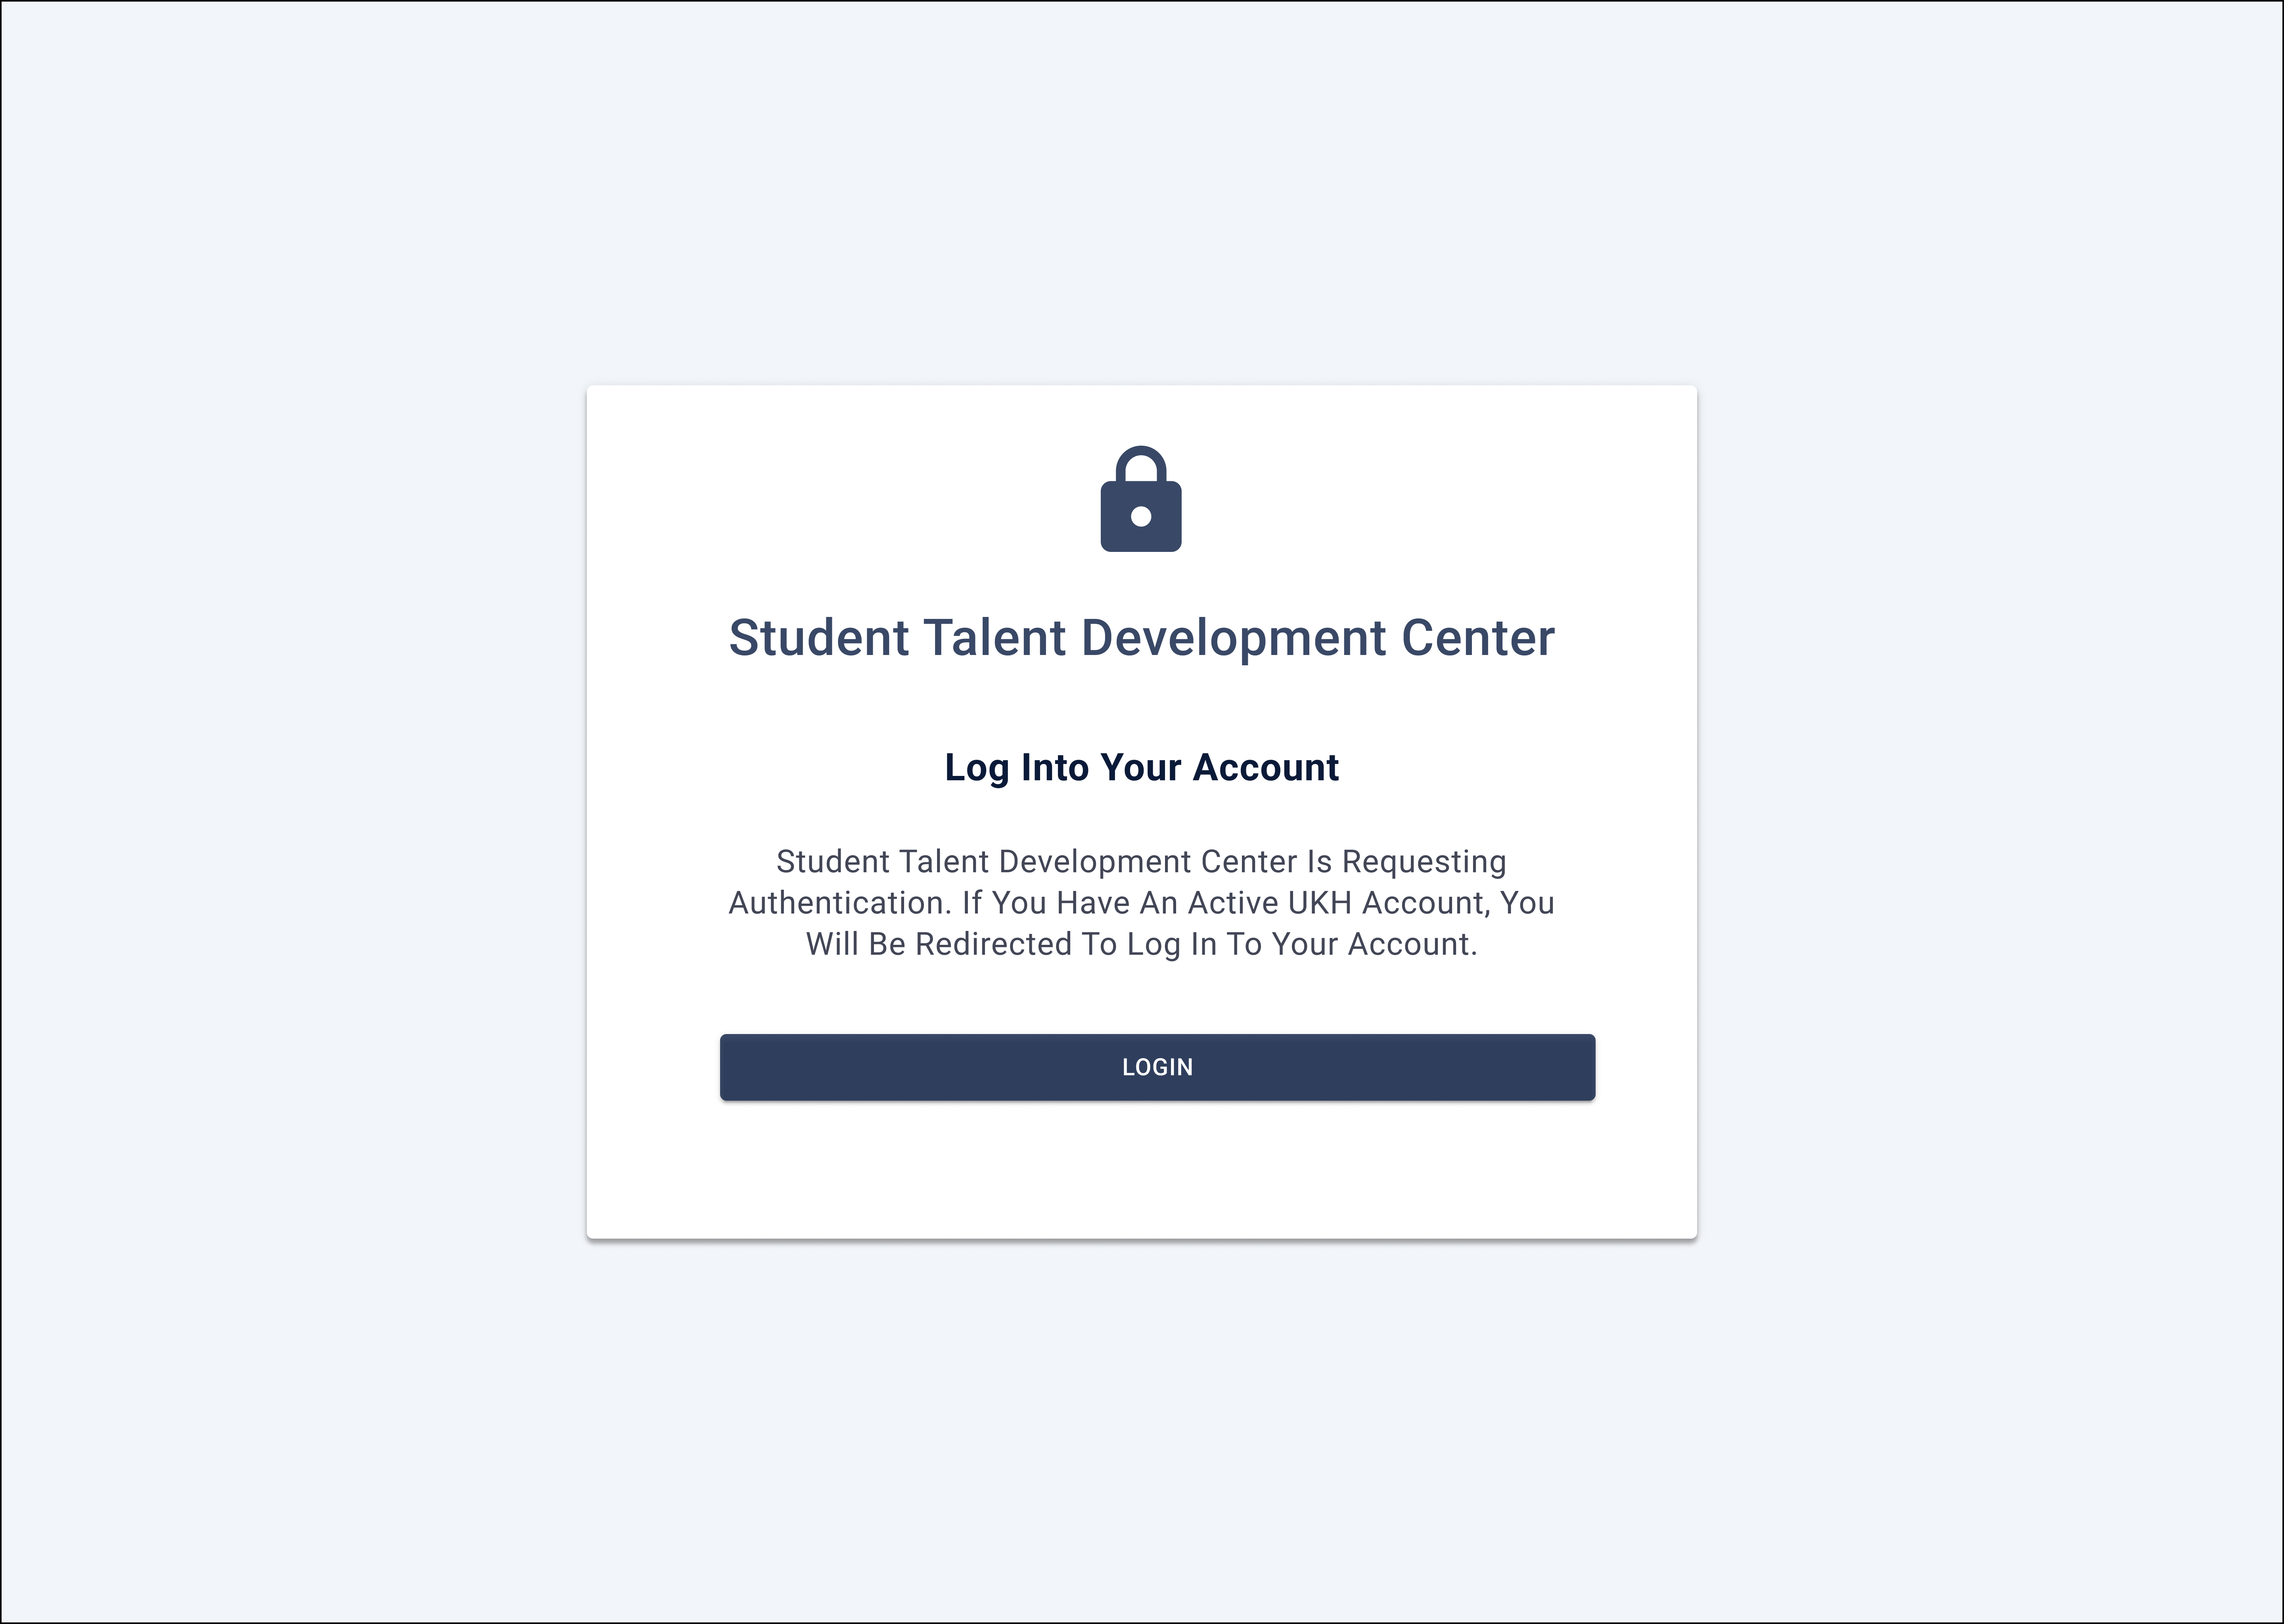
\includegraphics[width=150mm,scale=1]{figures/analysis_and_design/design/UI/1. Landing Page (UI01).png}}
    \caption{UI01. landing page (login)}
    \label{UI01}
    \end{figure}
    \clearpage


    \noindent\textbf{\textit{UI02. Home Page}}\newendline
    This page appears after user logs in, or when user clicks on “Home” button from the sidebar. This page shows a few important details, first the enrolled modules of the user. Second, it shows all the other modules that the user could enroll himself into. Users could search for modules by their name using the search bar. Users could also view any module in detail when they click on “View Module” button, this will redirect them to (UI09).\\

    \begin{figure}[H]
    \centerline{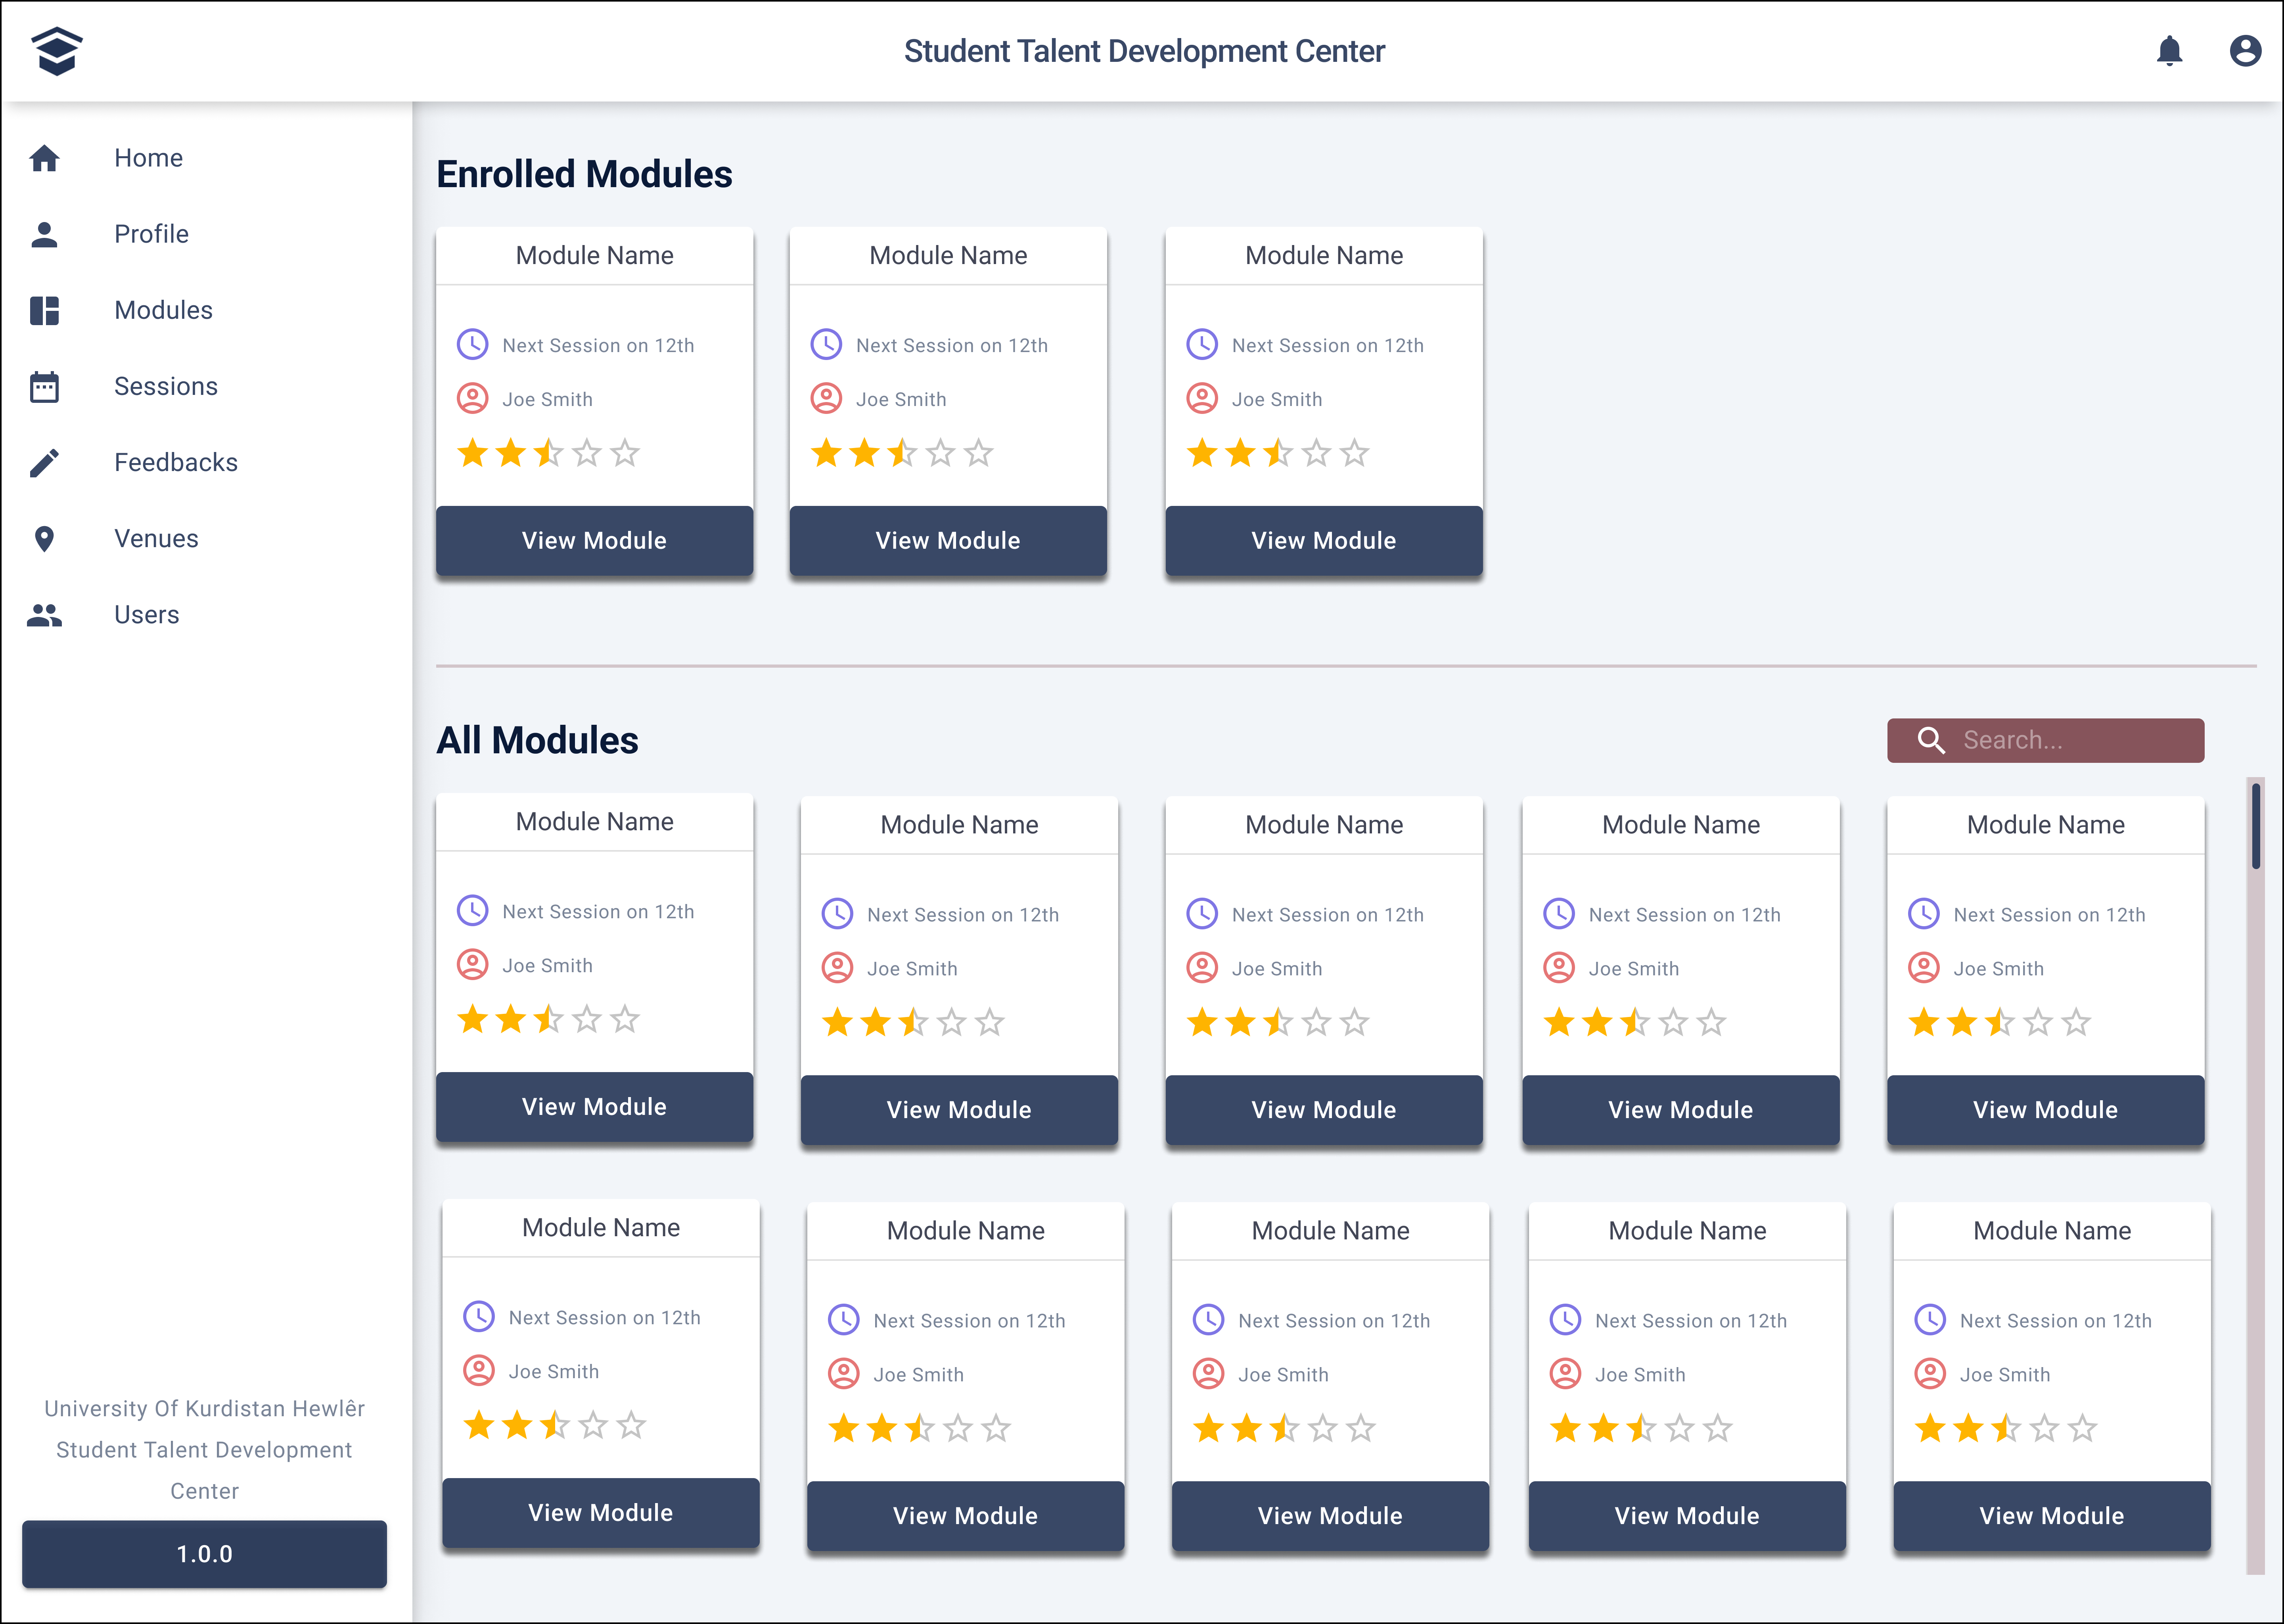
\includegraphics[width=150mm,scale=1]{figures/analysis_and_design/design/UI/2. Home Page (UI02).png}}
    \caption{UI02. home page}
    \label{UI02}
    \end{figure}
    \clearpage


    \noindent\textbf{\textit{UI03. Profile Page}}\newendline
    This page appears when user clicks on “Profile” button from the sidebar. This page shows a few important details, first the user’s details shown in the table below, including the user’s email, first name, last name, roles, and status of their account. Second, it shows all the hours that the tutor has tutored (this part doesn’t show when user views profile). Third, the amount of money the tutor to be paid is show to the user. Lastly, the enter availability button which take user to a form page like UI11, where tutor can enter their availability. This button is not visible to students or admin.\\

    \begin{figure}[H]
    \centerline{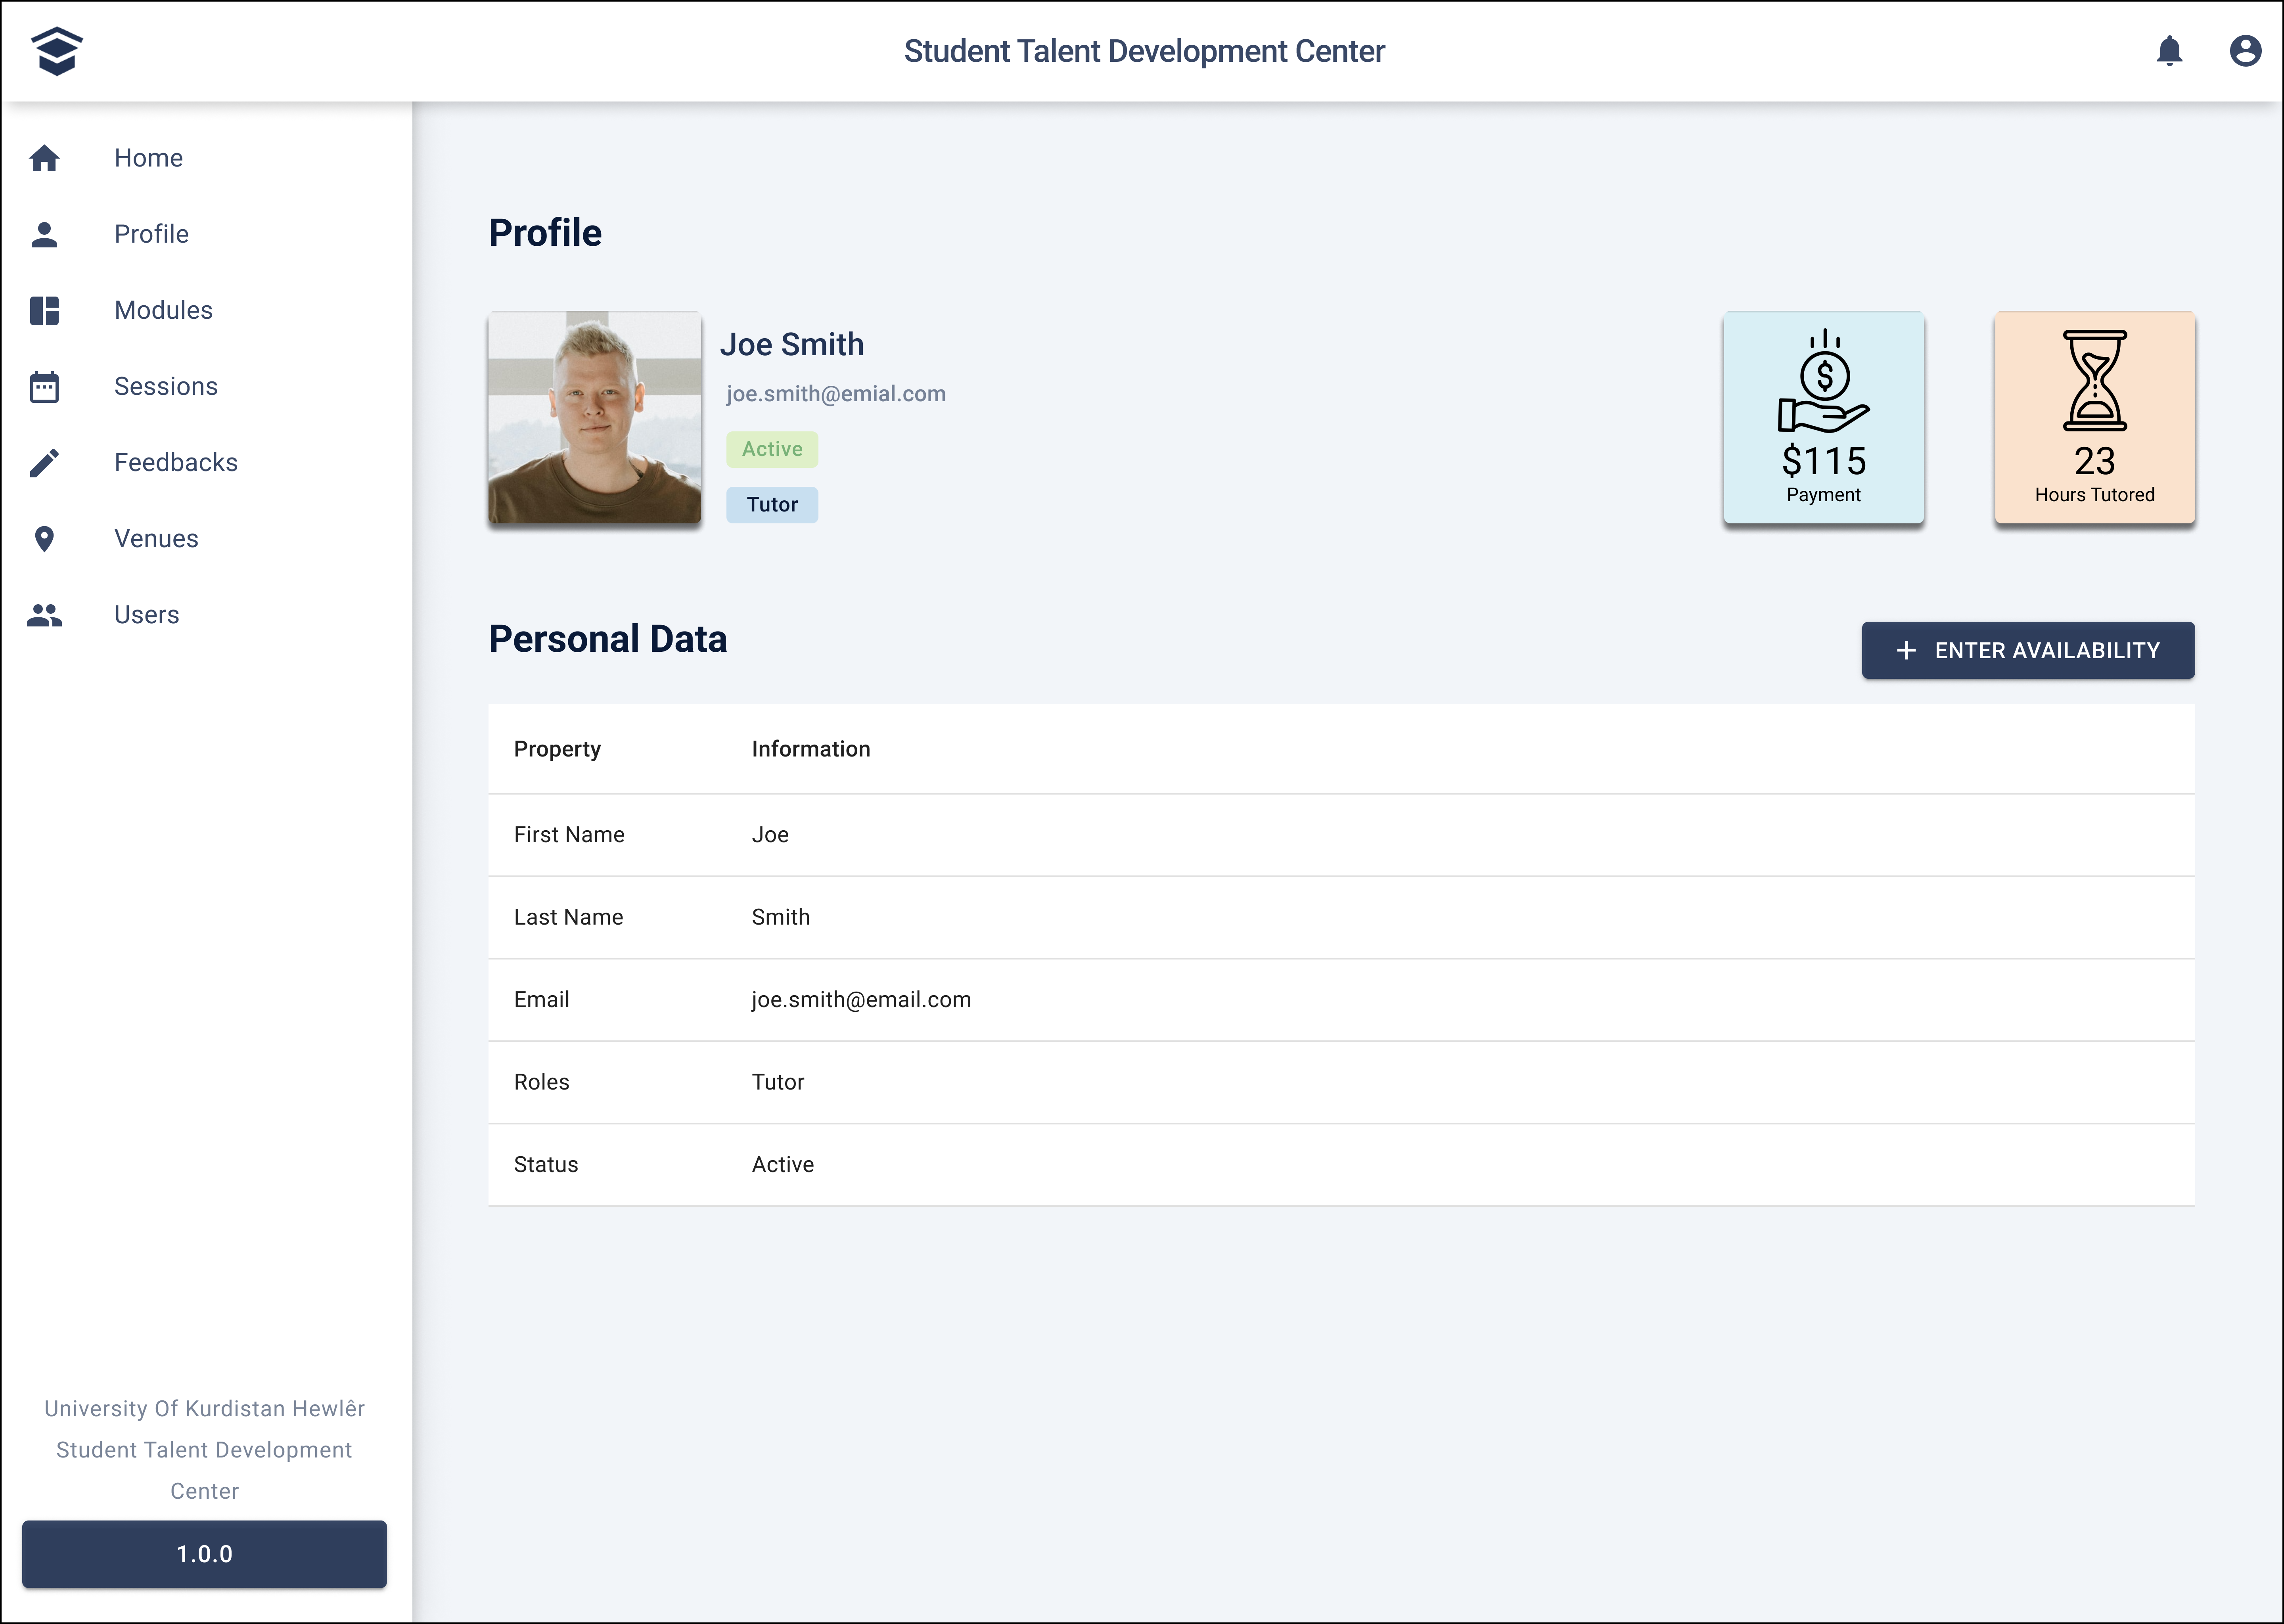
\includegraphics[width=150mm,scale=1]{figures/analysis_and_design/design/UI/3. Profile Page (UI03).png}}
    \caption{UI03. profile page}
    \label{UI03}
    \end{figure}
    \clearpage



    \noindent\textbf{\textit{UI04. Modules Page}}\newendline
   This page appears when user clicks on “Modules” button from the sidebar. This page shows all the existing modules. It allows the user (admin) to edit or delete a module. Additionally, the assign tutor button allows admin to assign a module to tutor (a form alike page will appear when clicked). User can search for modules based on name, and user can filter modules, the fields for both is abstracted away, when implemented, there might be many of these filtering fields. It is important to note that this page is only visible to admin, so is the button on the sidebar.\\

    \begin{figure}[H]
    \centerline{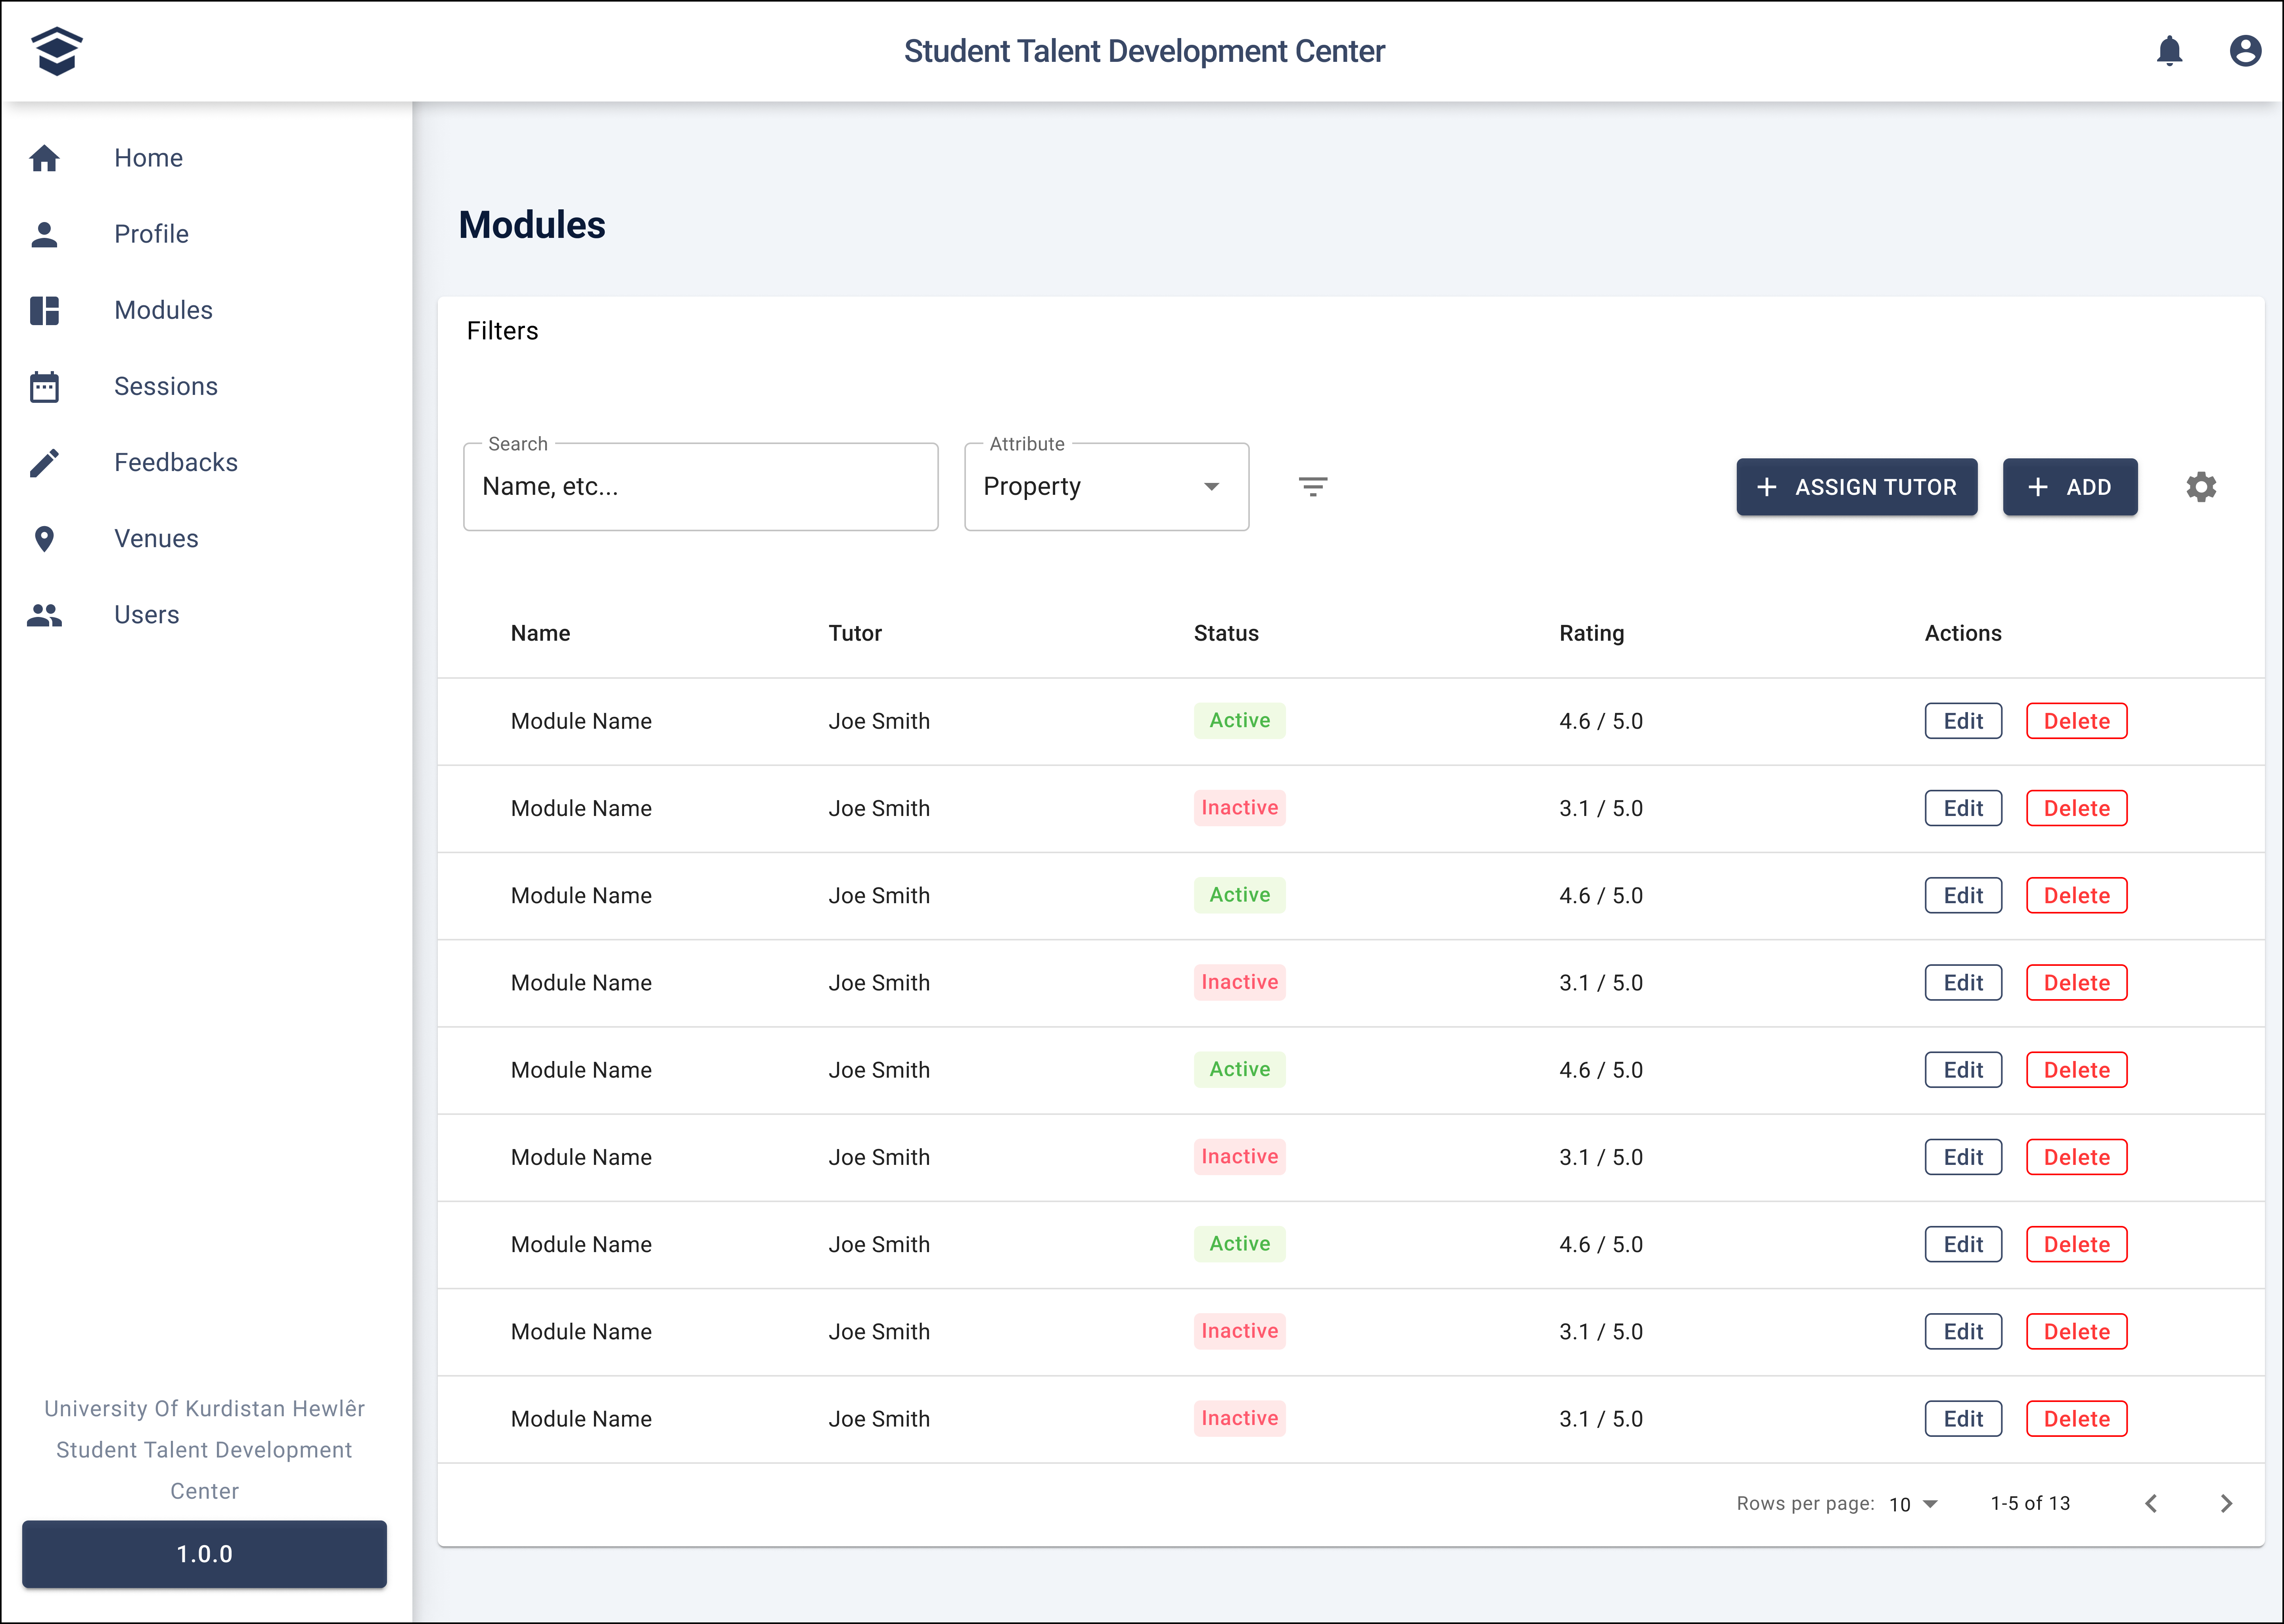
\includegraphics[width=150mm,scale=1]{figures/analysis_and_design/design/UI/4. Modules Page (UI04).png}}
    \caption{UI04. modules page}
    \label{UI04}
    \end{figure}
    \clearpage



    \noindent\textbf{\textit{UI05. Sessions Page}}\newendline
    This page appears when user clicks on “Sessions” button from the sidebar. This page shows all the upcoming sessions on top and then all of the existing sessions below that. It allows the user to view time and venue in short details. However, users have the ability to click on “View Session” button for further details (UI10).  Users can also click on the “View Session History” button to view the history of sessions attended. Users can also search for sessions using the search bar provided.\\

    \begin{figure}[H]
    \centerline{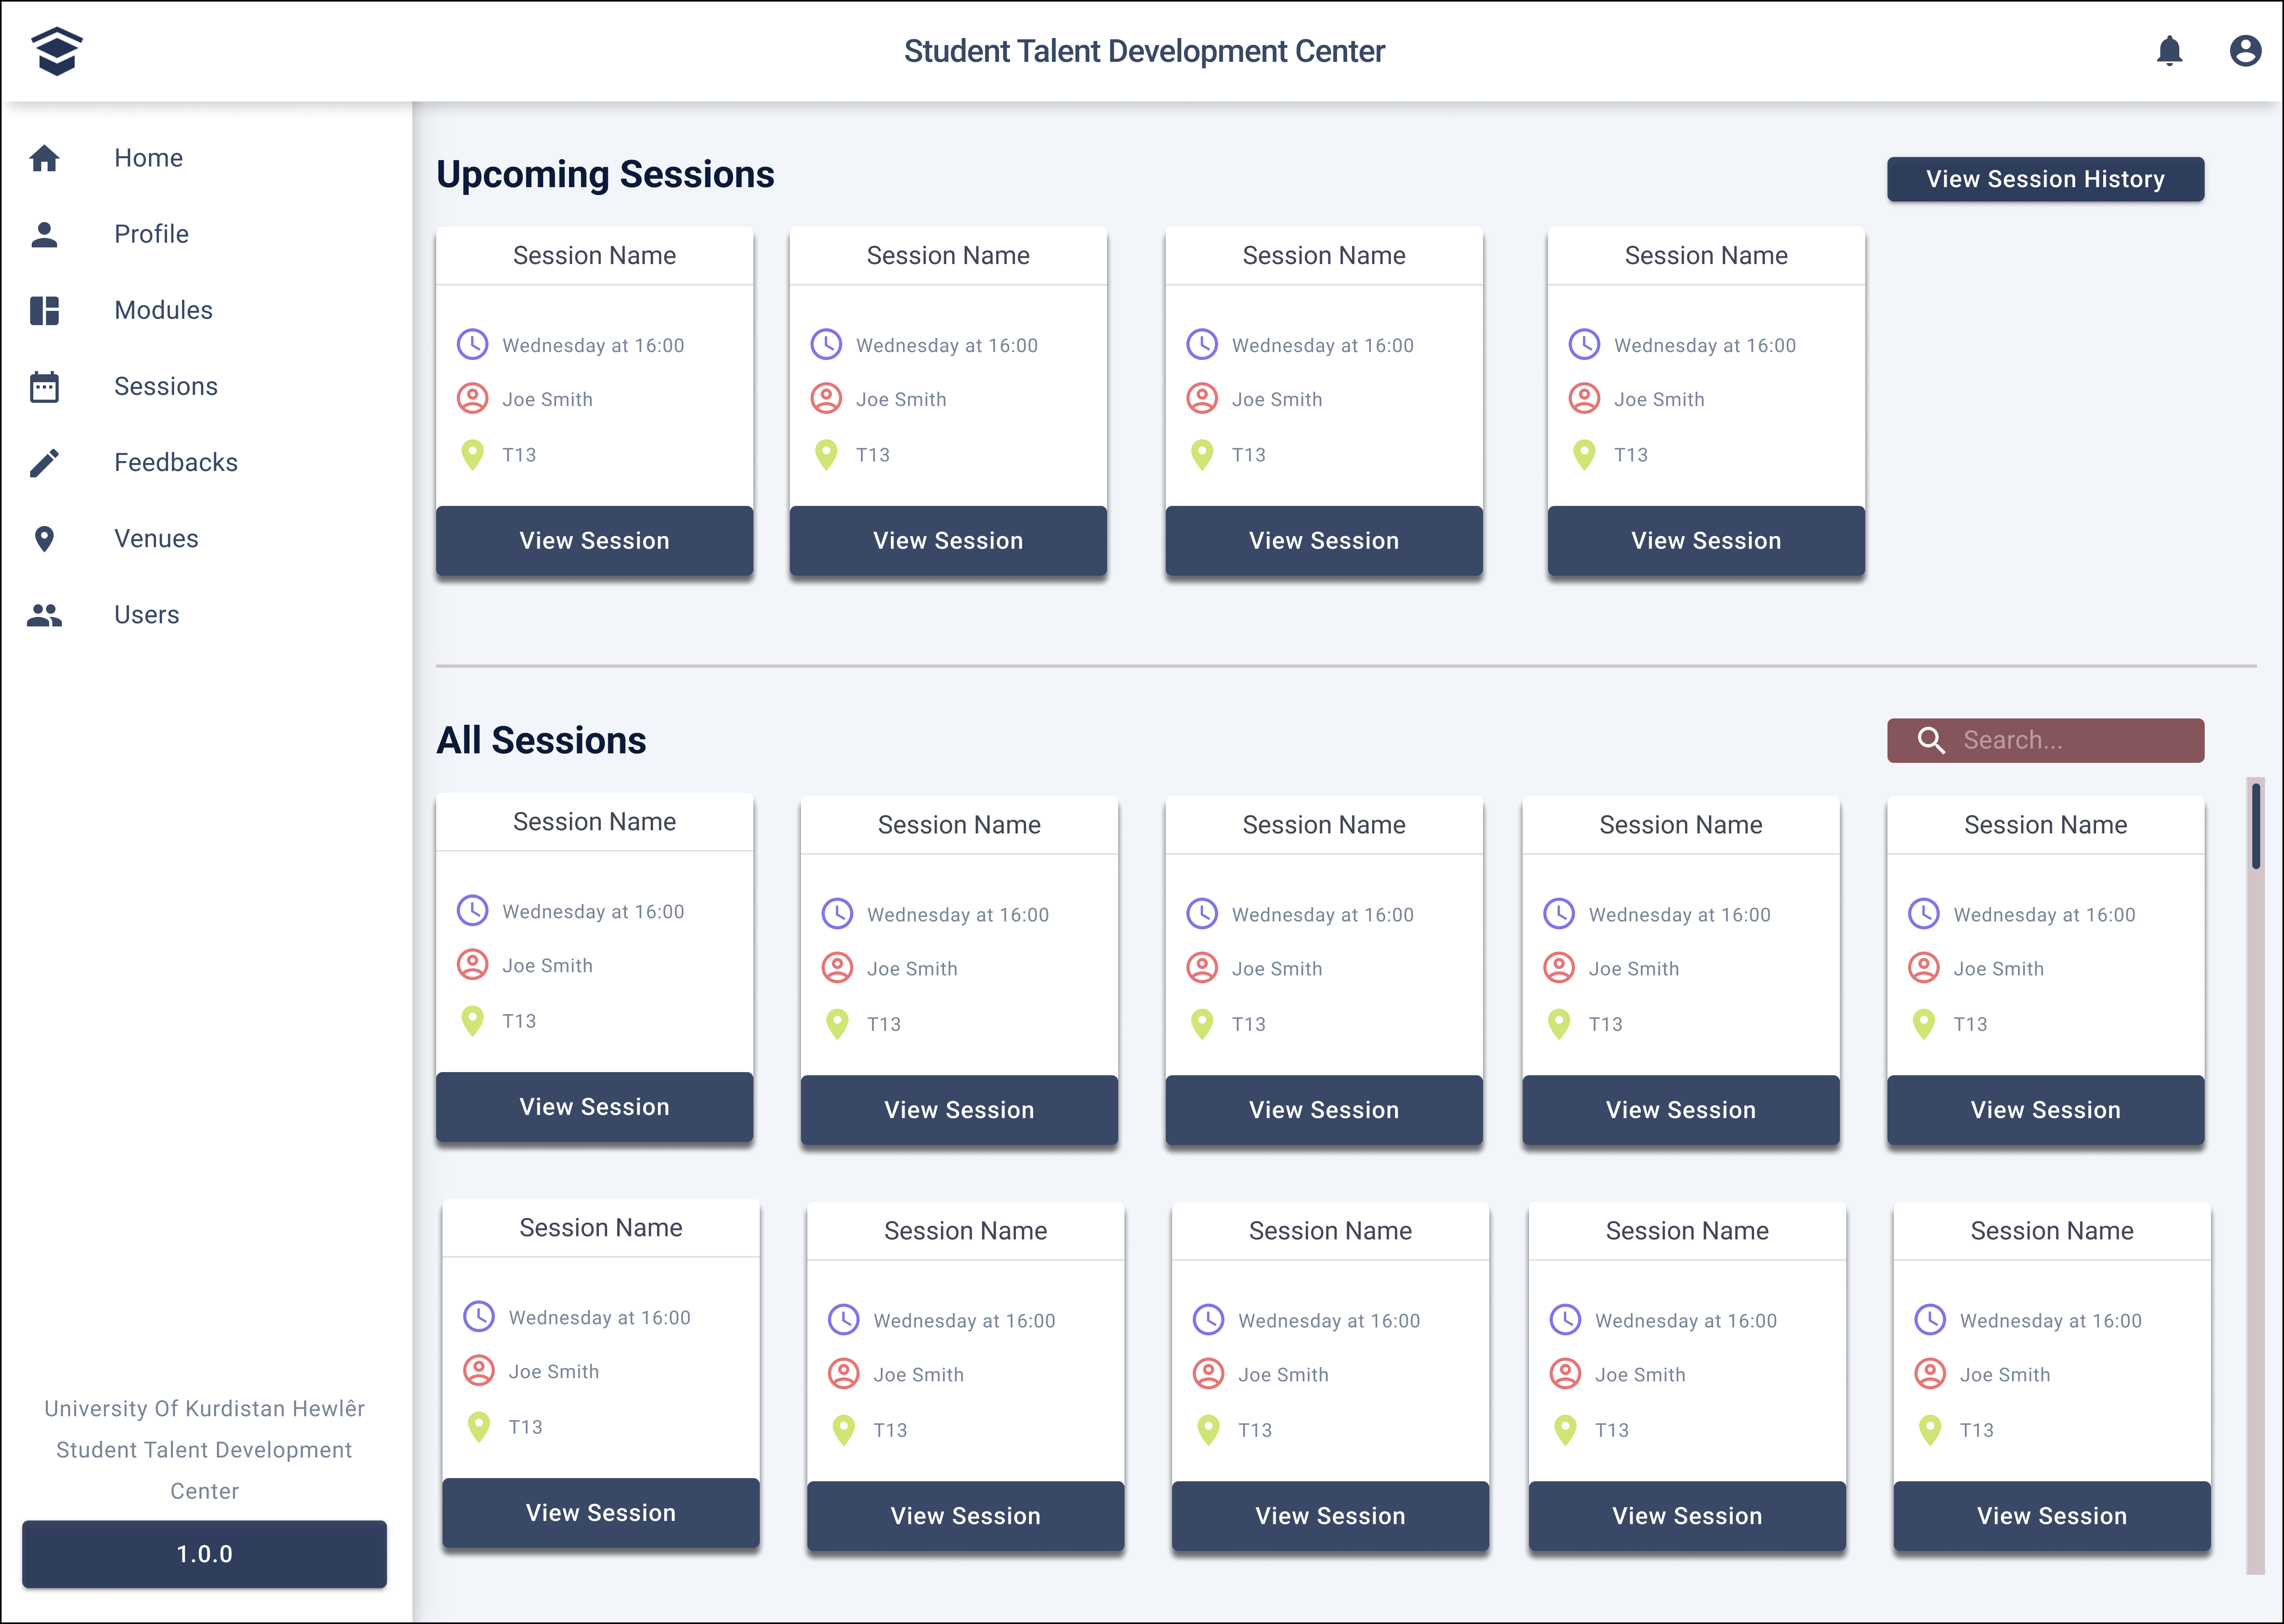
\includegraphics[width=150mm,scale=1]{figures/analysis_and_design/design/UI/5. Sessions Page (UI05).png}}
    \caption{UI05. sessions page}
    \label{UI05}
    \end{figure}
    \clearpage




    \noindent\textbf{\textit{UI06. Feedbacks Page}}\newendline
    This page appears when user clicks on “Feedbacks” button from the sidebar. This page shows all the received feedbacks. It allows the user (admin) to view feedback using the specified button. Additionally, admin can search for feedbacks and can filter feedbacks, the fields for both is abstracted away, when implemented, there might be many of these filtering fields. It is important to note that this page is only visible to admin, so is the button on the sidebar.\\

    \begin{figure}[H]
    \centerline{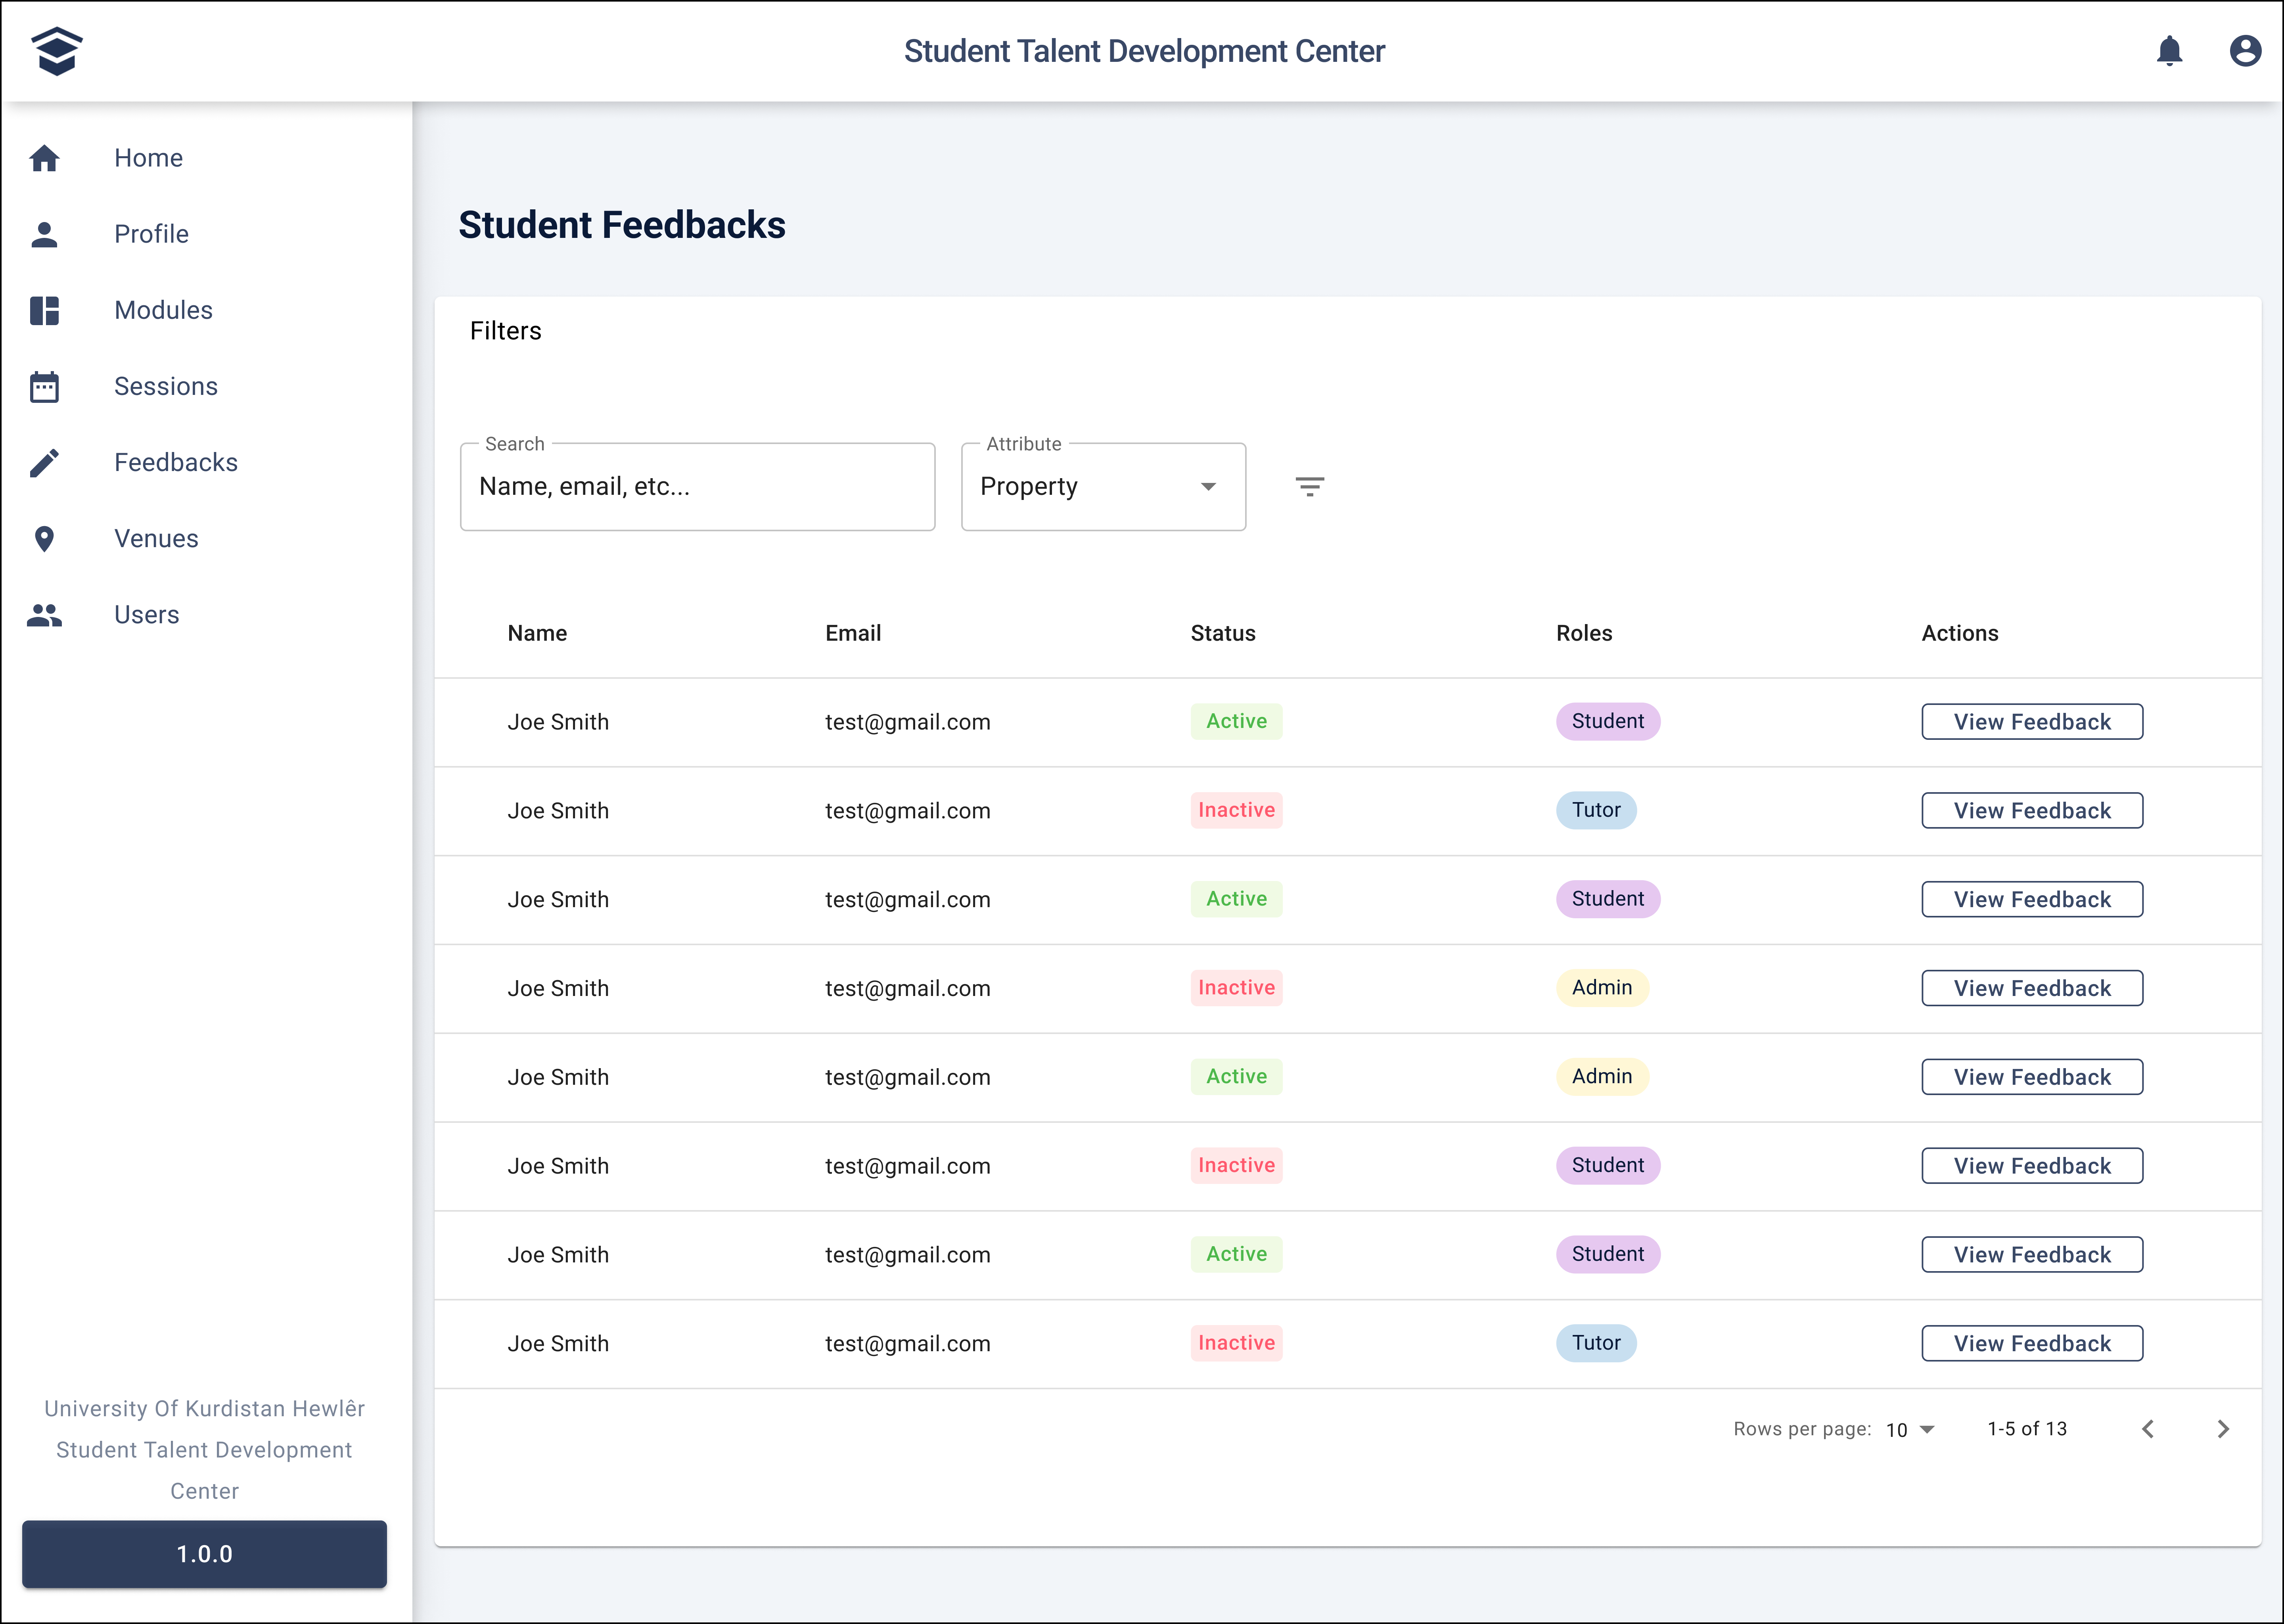
\includegraphics[width=150mm,scale=1]{figures/analysis_and_design/design/UI/6. Feedbacks Page (UI06).png}}
    \caption{UI6. feedbacks page}
    \label{UI06}
    \end{figure}
    \clearpage




    \noindent\textbf{\textit{UI07. Venues Page}}\newendline
    This page appears when user clicks on “Venues” button from the sidebar. This page shows all the existing venues. It allows the user (admin) to edit or delete a venue. Additionally, the new button allows admin to add a new venue (a form alike page will appear when clicked). User (admin) can search for venues based on name, and user can filter venues, the fields for both is abstracted away, when implemented, there might be many of these filtering fields. It is important to note that this page is only visible to admin, so is the button on the sidebar.\\

    \begin{figure}[H]
    \centerline{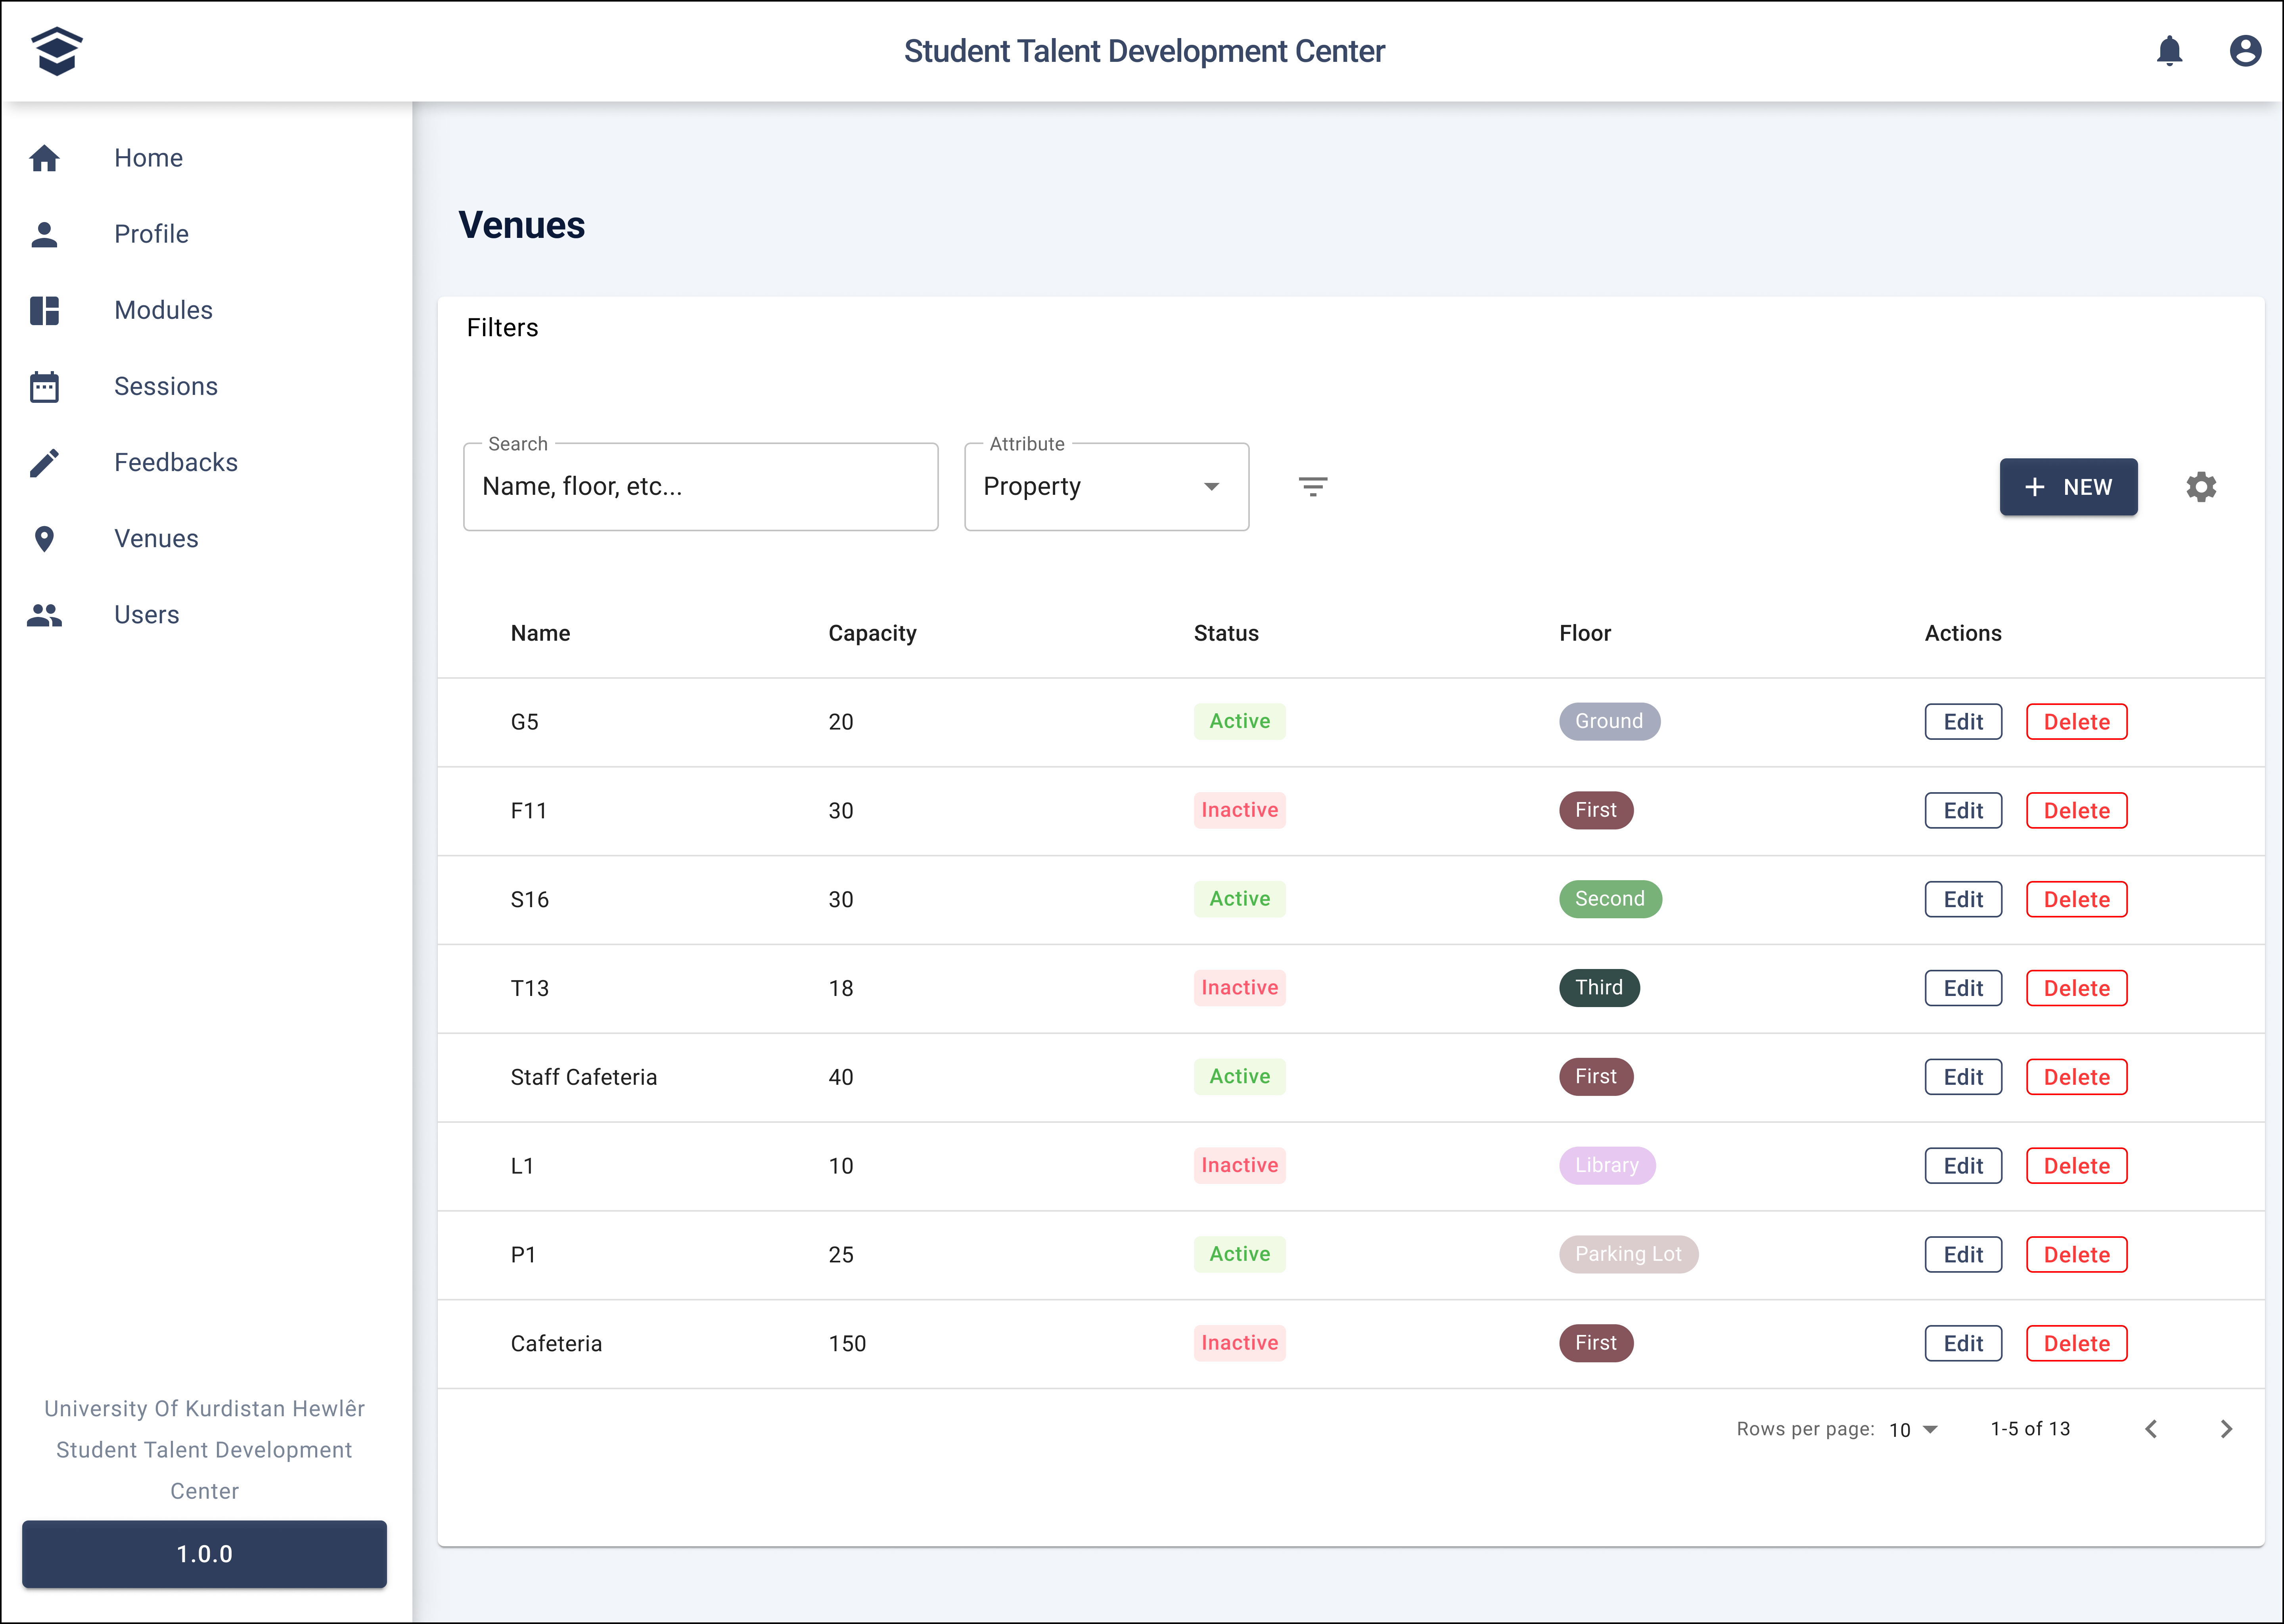
\includegraphics[width=150mm,scale=1]{figures/analysis_and_design/design/UI/7. Venues Page (UI07).png}}
    \caption{UI07. venues page}
    \label{UI07}
    \end{figure}
    \clearpage




    \noindent\textbf{\textit{UI08. Users Page}}\newendline
    This page appears when user clicks on “Users” button from the sidebar. This page shows all of the enrolled users. It allows the user (admin) to update a user’s information, or to add a user. Additionally, the “Onboard Tutor” button allows admin to onboard a user as a tutor (a form alike page will appear when clicked). Admin can search for users based on name, and can filter users, the fields for both is abstracted away, when implemented, there might be many of these filtering fields. It is important to note that this page is only visible to admin, so is the button on the sidebar.\\

    \begin{figure}[H]
    \centerline{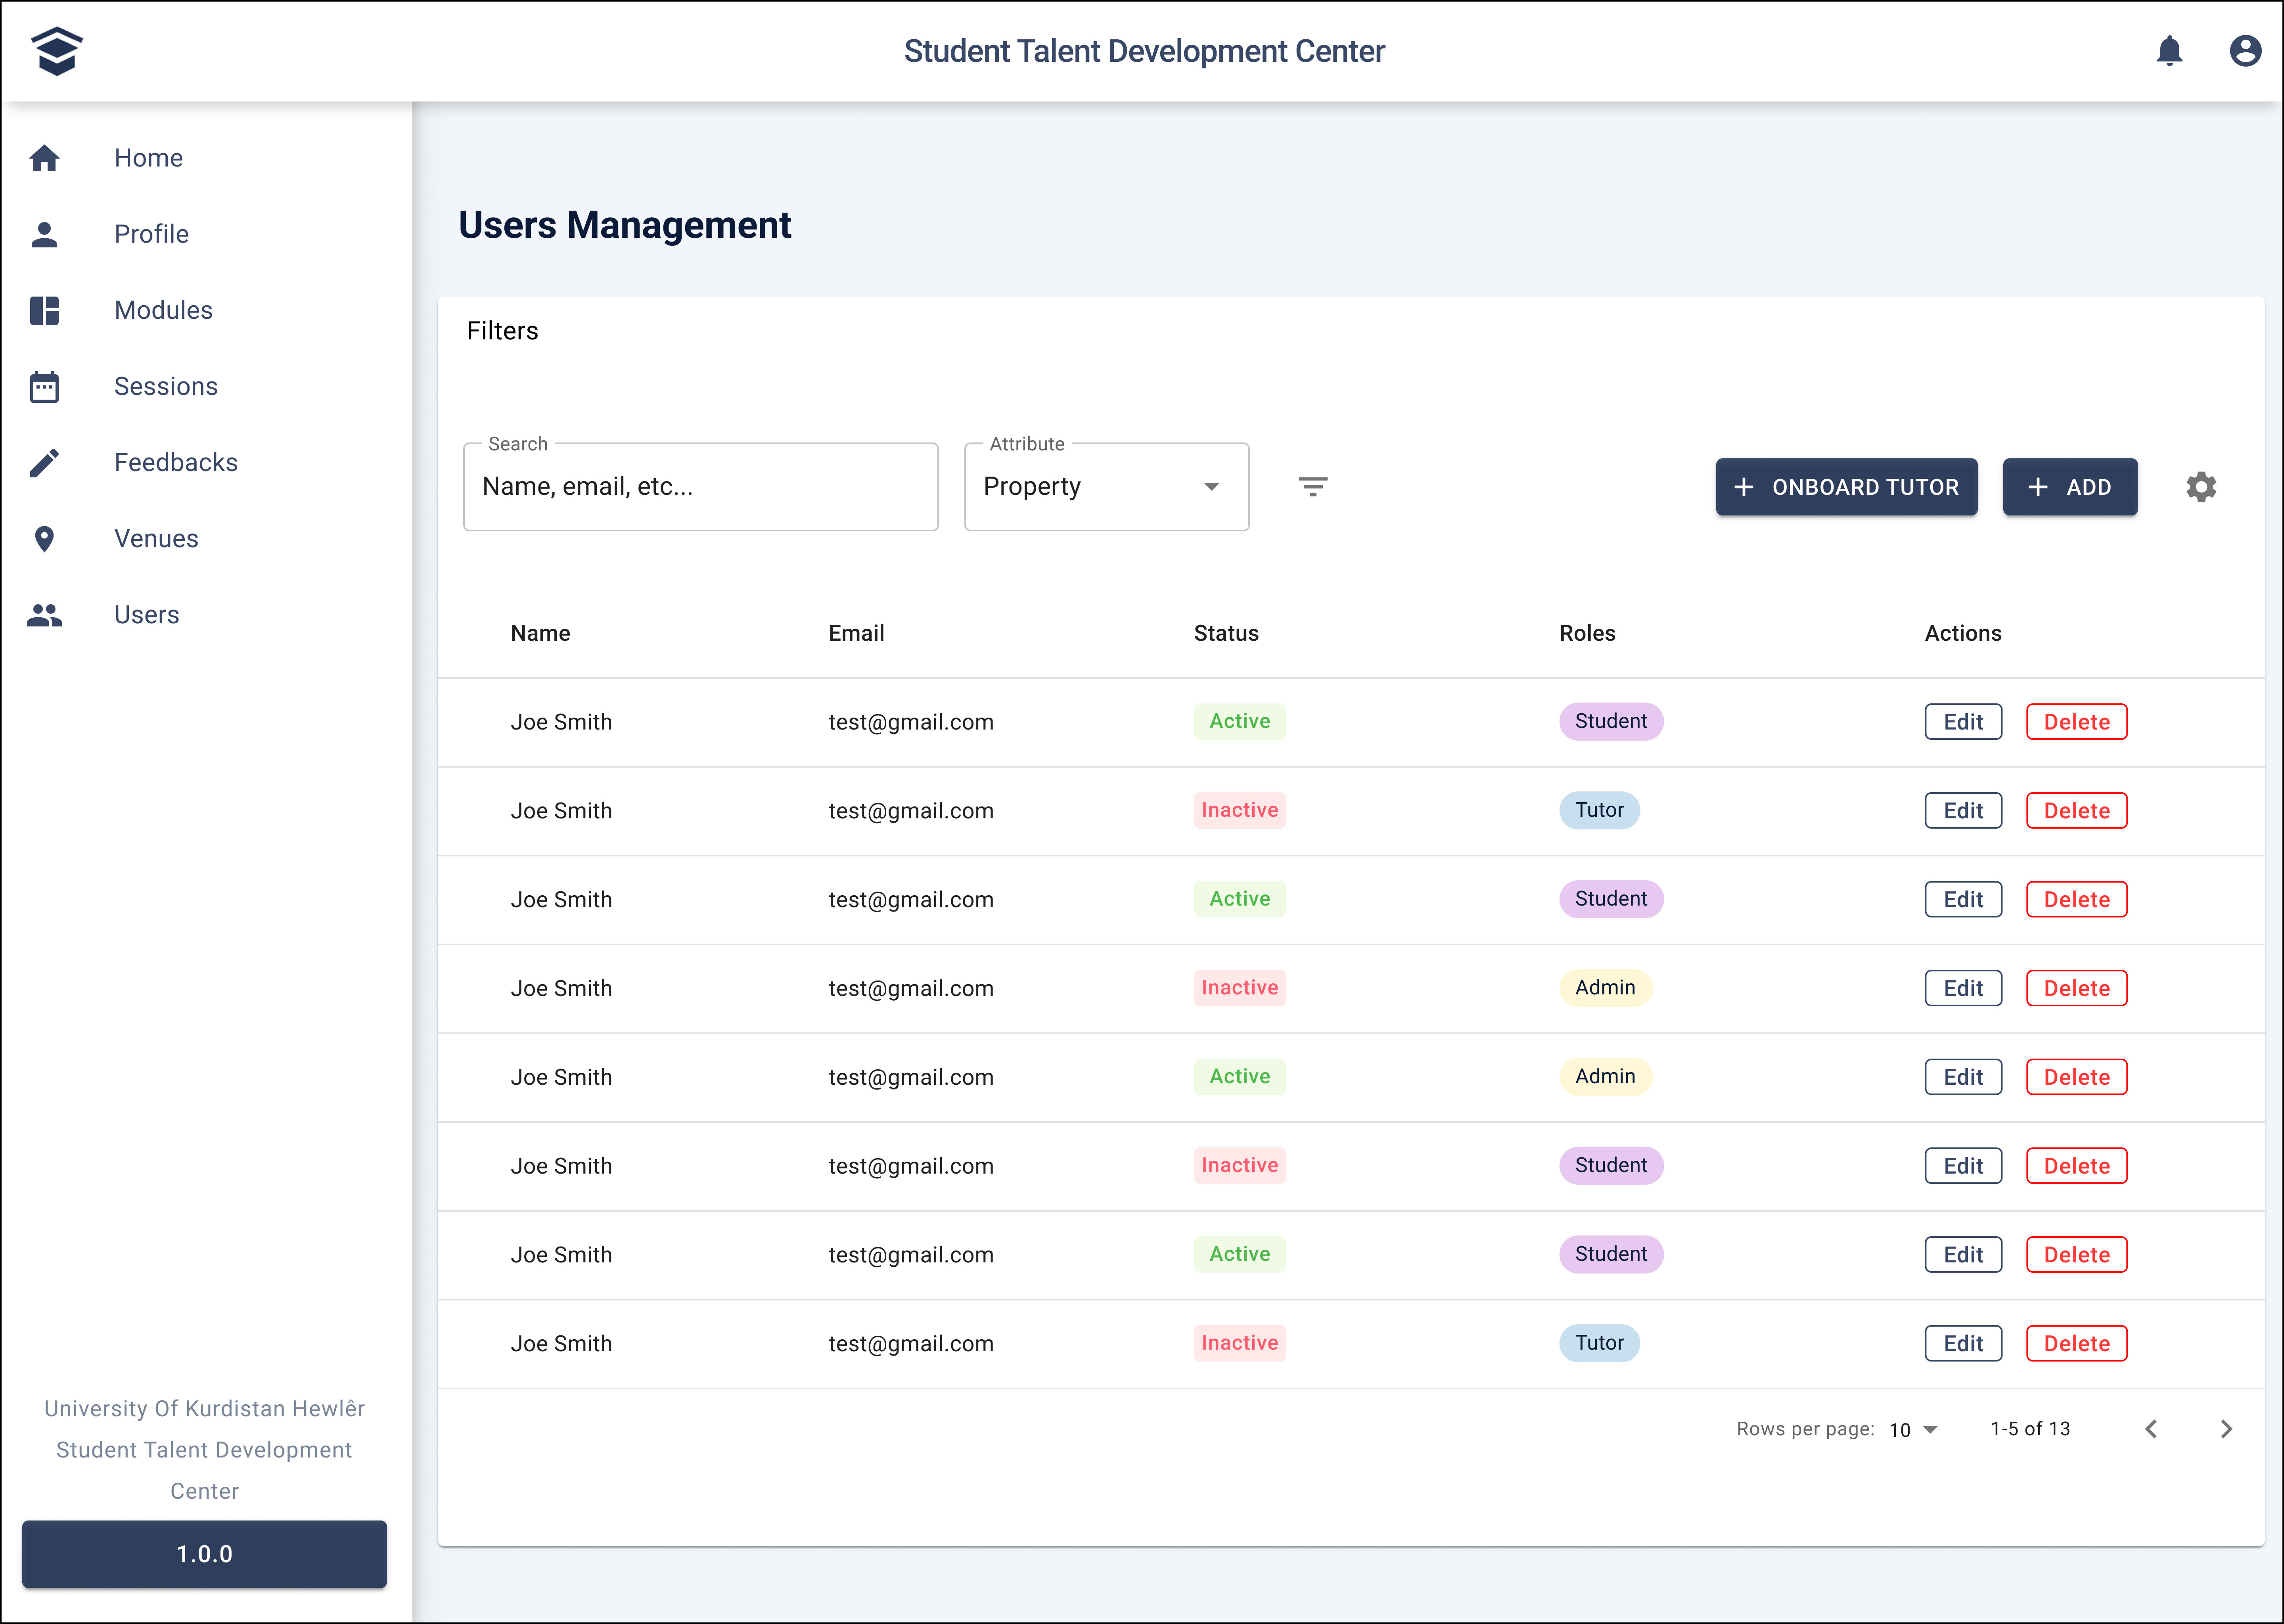
\includegraphics[width=150mm,scale=1]{figures/analysis_and_design/design/UI/8. Users Page (UI08).png}}
    \caption{UI08. users page}
    \label{UI08}
    \end{figure}
    \clearpage



    \noindent\textbf{\textit{UI09. View Module Page}}\newendline
    This page appears when user clicks on “View Module” button from the modules page. This page shows all of the information of a module, and show all of its sessions. It also allows the users view its properties in a tabular format when “properties” is clicked. Additionally, the “Assign Tutor” button allows admin to assign a tutor for a module (a form alike page will appear when clicked). Admin can search for sessions using the search bar, and can view the sessions. It is important to note that the button on the top right “Assign Tutor” is only available to admin.\\

    \begin{figure}[H]
    \centerline{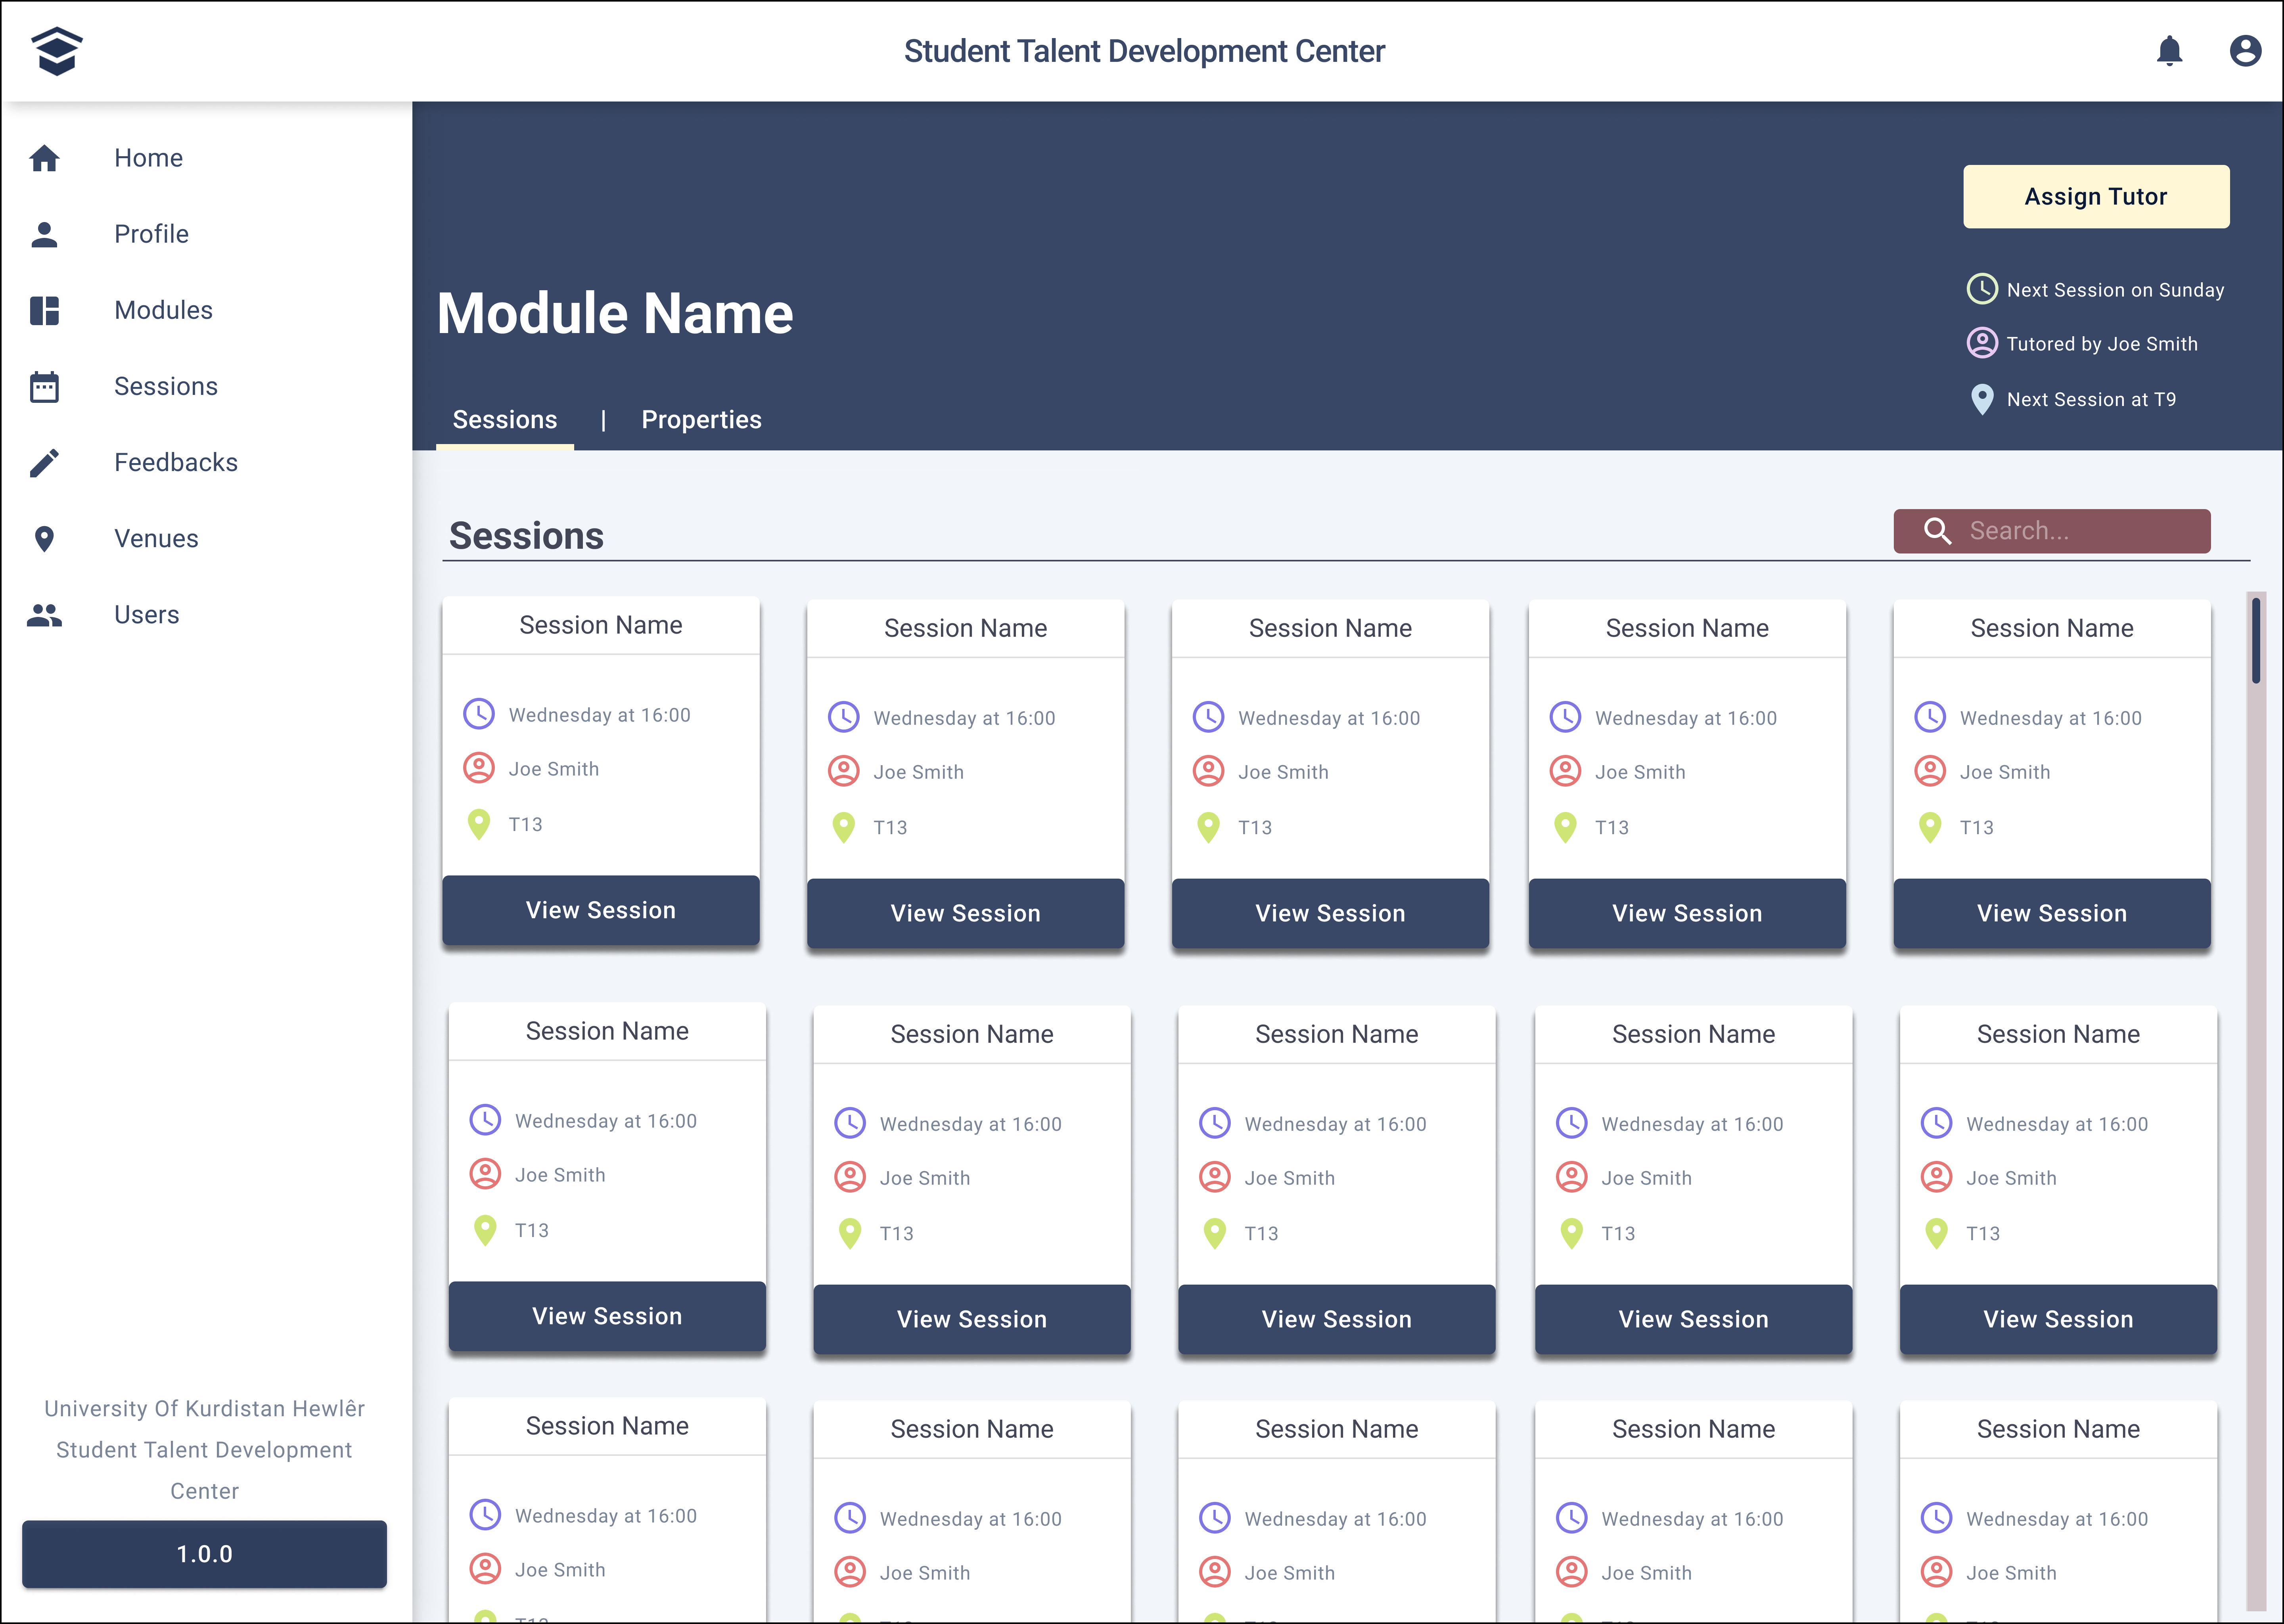
\includegraphics[width=150mm,scale=1]{figures/analysis_and_design/design/UI/9. View Module Page (UI09).png}}
    \caption{UI09. view module page}
    \label{UI09}
    \end{figure}
    \clearpage


    \noindent\textbf{\textit{UI10. View Session Page}}\newendline
    This page appears when user clicks on “View Session” button from the modules page and sessions page. This page shows all of the information of a session. Additionally, users have access to a few tabs of the session including materials, attendance, provide feedback, assign time and venue, and upload material with addition to the cancel session button on top right corner. These are all different actions to take when this page is viewed. Note that not all of these are available to all the users. Cancel Session is allowed for Tutor, Assign Time and Venue is only allowed for admin, Provide Feedback only to student, and so on.\\
    \begin{figure}[H]
    \centerline{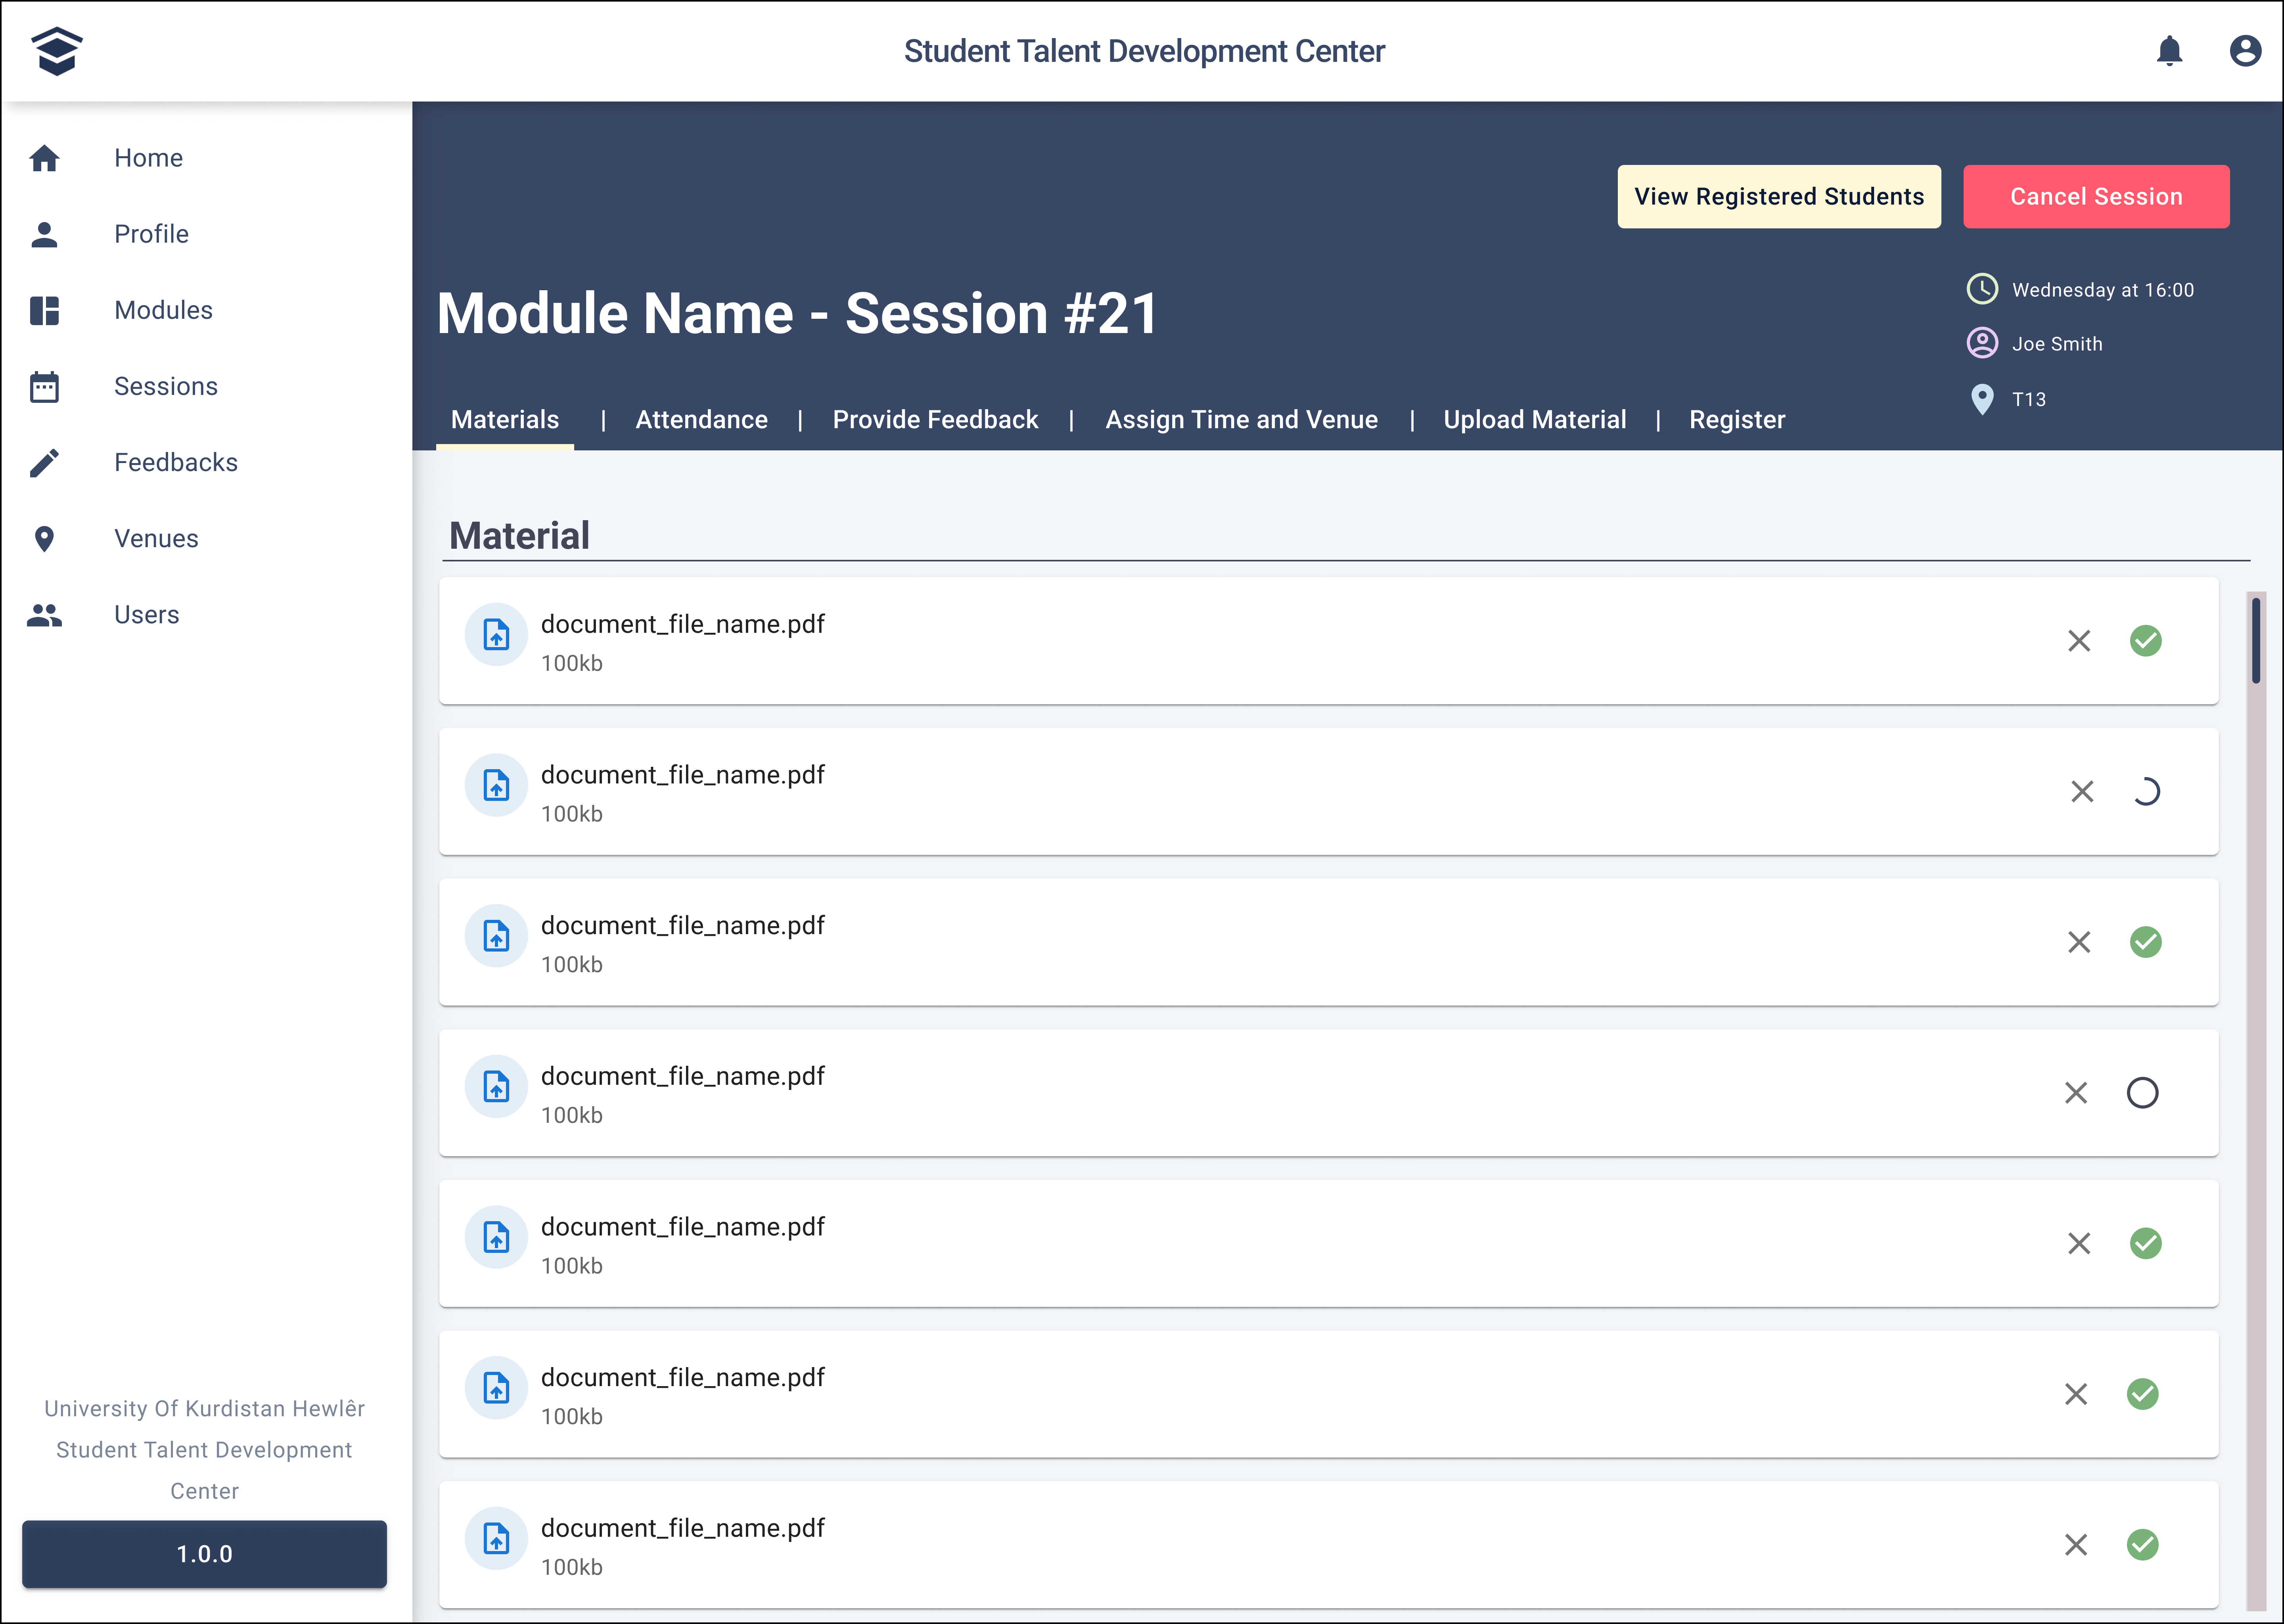
\includegraphics[width=150mm,scale=1]{figures/analysis_and_design/design/UI/10. View Session Page (UI10).png}}
    \caption{UI10. view session page}
    \label{UI10}
    \end{figure}
    \clearpage

    \noindent\textbf{\textit{UI11. Form Page}}\newendline
    This page appears after user is faced with a form alike page. This includes creation, adding, updating, editing, providing feedback, entering availability, assignment features, and so on. The properties of this page vary depending on the form fields; however, the representation below should give a good overall structure and look of these forms. When a required field is left empty, the field outline turns red and the text “required” appear under that field.\\

    \begin{figure}[H]
    \centerline{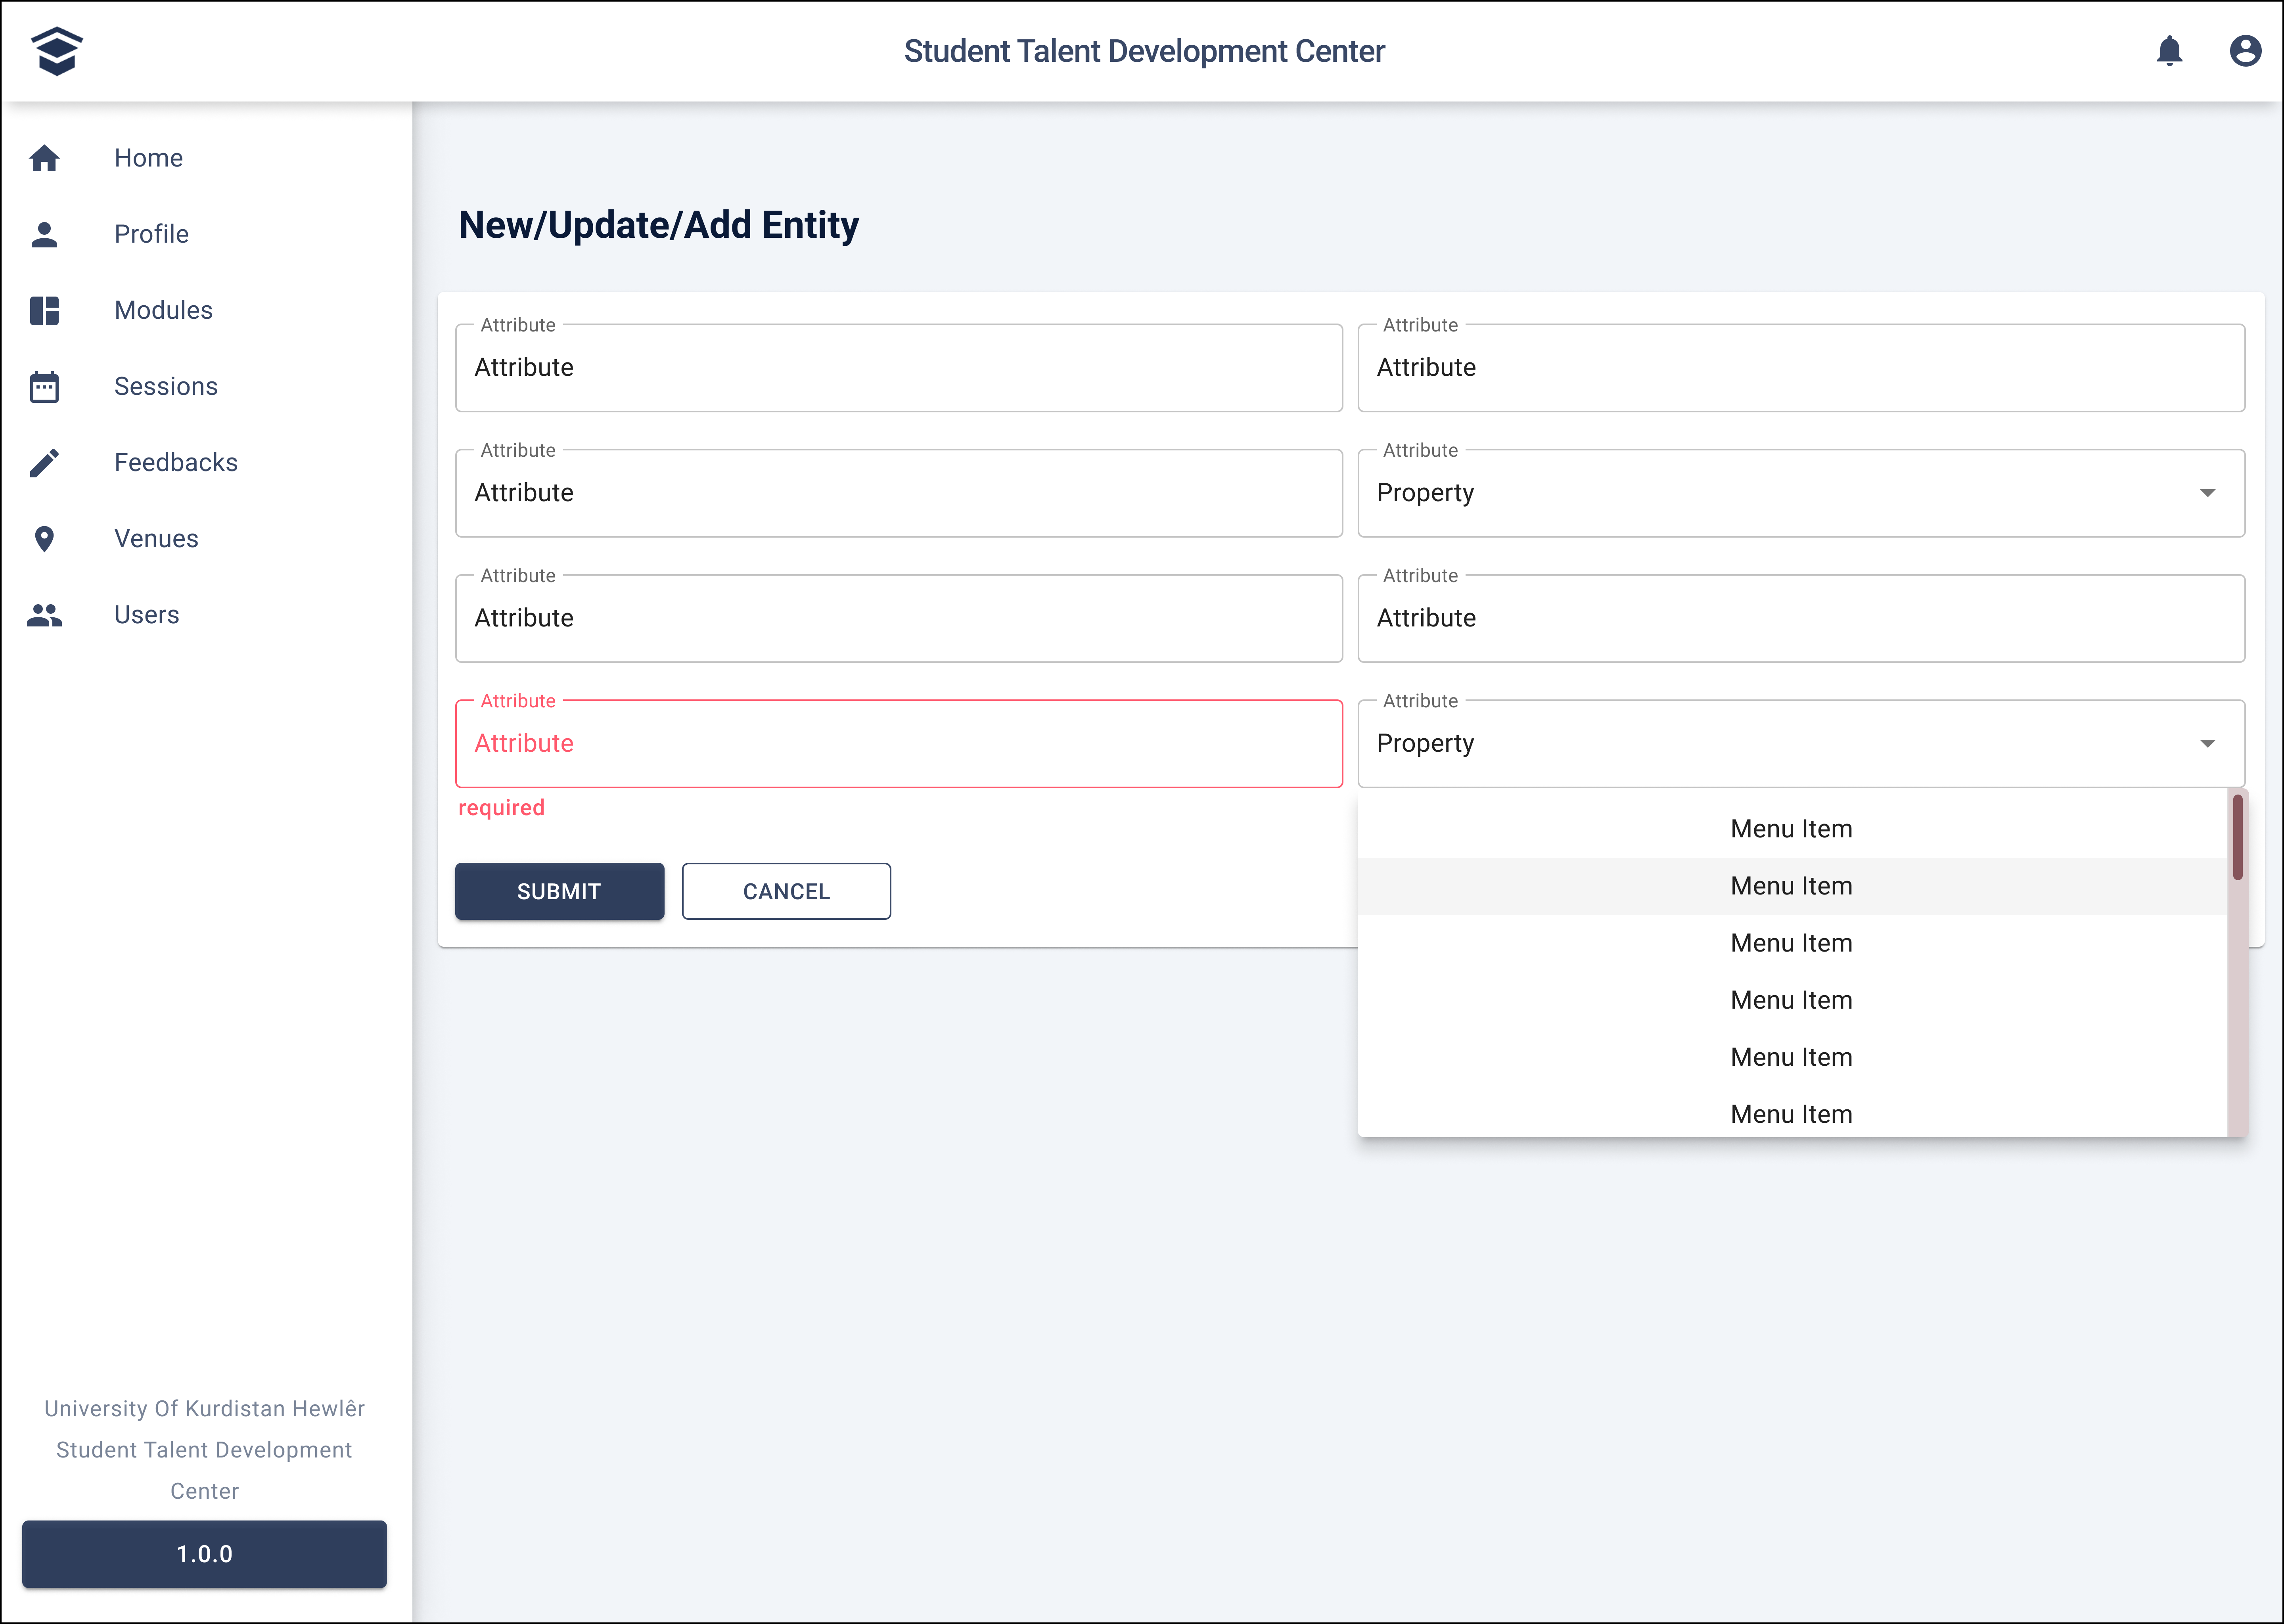
\includegraphics[width=150mm,scale=1]{figures/analysis_and_design/design/UI/11. Form Page (UI11).png}}
    \caption{UI11. form page}
    \label{UI11}
    \end{figure}
    \clearpage

\end{justify}
\clearpage

\subsection{Database Design}
\begin{justify}
The following is the Database Design of the Student Talent Development Center Web Application. First, the strategy for mapping the object to relational tables is discussed. Secondly, attention is given to the logical modelling where the persistent entities are defined, then the relationship between entities is highlighted. Lastly, the physical modelling will be illustrated where the data types of the attributes are set.

\vspace{0.25cm}
\newendline \textbf{\textit{Mapping Objects to Relational Tables}}\newendline
The Student Talent Development Center Web Application is constructed being developed using Object oriented principles and utilizes a relational database management system (RDBMS) to store data persistently. The connecting of objects and tables is going to be handled by an "object-relational mapping layer" (ORM) that will be a part of STDC. The primary goal of this layer would be to simplify and speed up the mapping procedure while also providing an abstraction that would insulate users from the implementation specifics of the mapping. One aspect of this is the relationship and data type mapping. This mapping procedure is, to a certain degree, simple. Object-oriented class inheritance, also known as generalization, stands out as a relationship type that needs extra care.

\vspace{0.25cm}
\newendline {\textit{Property Mapping}}\\
It is decided that each persistent attribute of an object will be mapped to a column in the database tables. This will ensure that object properties are mapped correctly inside the system. To put it more simply, a mapping of a single column to a single attribute. The attributes, also known as properties, are considered to be persistent when they maintain their presence after the execution process has been completed. Additionally, metadata will be persisted and kept in the database as they are in the object.

\vspace{0.25cm}
\newendline {\textit{Relationship Mapping}}\\
In spite of the fact that the student talent development center does not yet have persistent class inheritance at this stage, it is essential to choose a mapping technique for inheritance classes before proceeding with any extension. It is possible to map inherited classes into their tables in one of three different ways: either by mapping the hierarchy of classes to a single table, mapping each concrete class to its own table, or mapping each class to its own table. The latter method, in which each table is mapped to one of its own tables, is the one that will be used by STDC. Conceptually, this is the mapping that comes the closest to inheritance. In addition to understanding mapping of properties and inheritance, it is required to have a solid grasp of the relationship mapping of various kinds of associations. Association, aggregation, and composition are the three different kinds of object relationships that need to be mapped. Because of how they are mapped in this application, each and every one of them will be handled in the exact same manner.  When it comes to mapping, STDC is interested in two different sorts of object relationships. These categories are: The first category is one that is founded on the concept of multiplicity, and it consists of three different sorts. Relationships that are one-to-one, those that are one-to-many, and those that are many-to-many are all possible. The second category is one that is focused on directionality, and within this category there are two different kinds of relationships: uni-directional and bi-directional relationships.\newendline
In conclusion, classes are mapped one to one with tables based on their multiplicity and directions, objects are mapped one to one if they are persistent after execution.

\vspace{0.25cm}
\newendline \textbf{\textit{Database Logical Model}}\newendline
The below model is the Entity Attribute Relationship Diagram which is derived from the class diagram (in Program Design). Each entity is a persistent entity in the database along with their attributes. Note that enumeration classes are not referred to here in the EARD for the sake of simplicity of the model due to its repetitive nature. The relationship between each entity is further explained after the below figure.

    \begin{figure}[H]
    \centerline{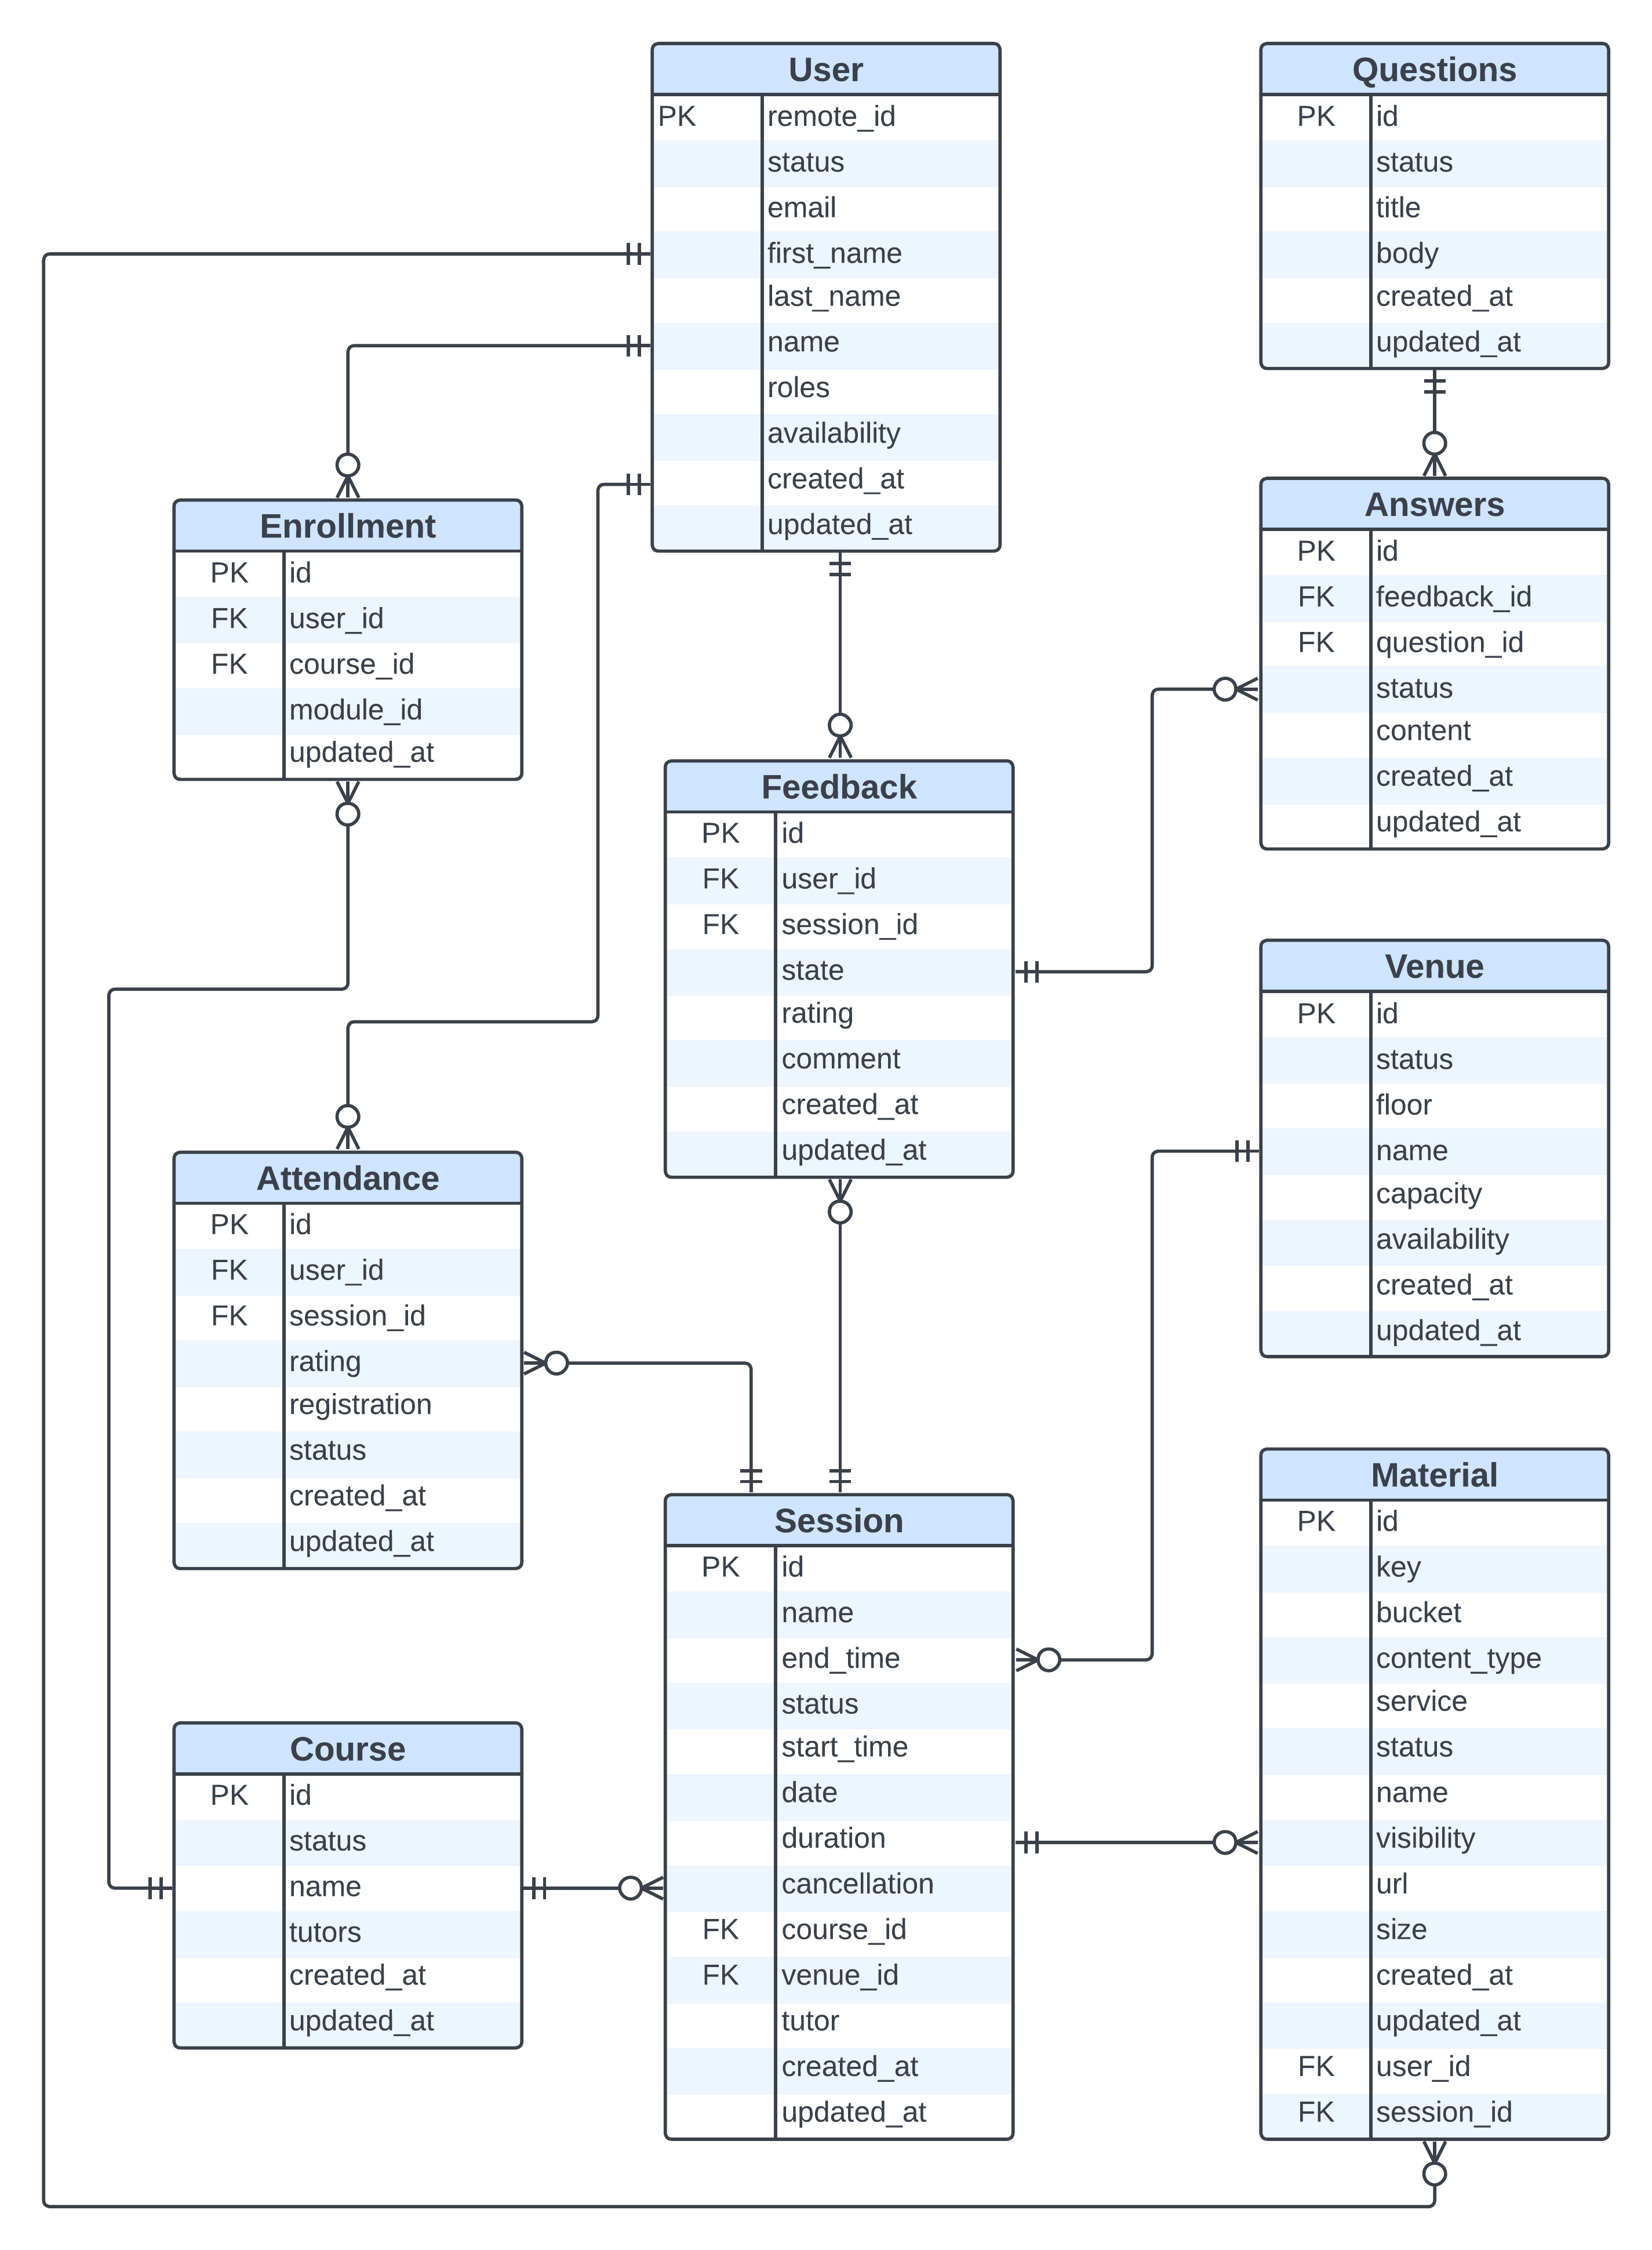
\includegraphics[width=145mm,scale=1]{figures/analysis_and_design/design/1. Logical Enitiy Attribute Relationship Diagram V2.png}}
    \caption{Database -- logical entity attribute relationship diagram}
    \label{logicalEARD}
    \end{figure}
\vspace{-0.5cm}
\begin{enumerate}
    \item User -- Feedback
        \begin{enumerate}[itemsep=-0.3cm]
            \item Each user can provide zero or many feedbacks.
            \item Each feedback submitted belong to one user and one only.

            \newendline Each feedback received has a unique id. User cannot provide multiple feedbacks to the same session.
        \end{enumerate}
    

    \item User -- Material
        \begin{enumerate}[itemsep=-0.3cm]
            \item Each user (tutor) can upload zero or many materials.
            \item Each material uploaded belongs to one user and one only.

            \newendline Each material received has a unique id. User can upload multiple materials to the same session each with different id.
        \end{enumerate}

    \item User -- Course
        \begin{enumerate}
            \item Each user (tutor) can tutor many courses.
            \item Each course is tutored by many users (tutors) considering the fact that in the upcoming years, tutor will change for a module. History of tutors of a course should be track-able for future extendibility.

            \newendline The many to many relationships between these is resolved by having the third table Enrollment. Each entry here will have a unique id.
        \end{enumerate}
        
    \item User -- Session
        \begin{enumerate}
            \item Each user (student) can attend zero or many sessions.
            \item Each session can have zero or many users (attendees).

            \newendline The many to many relationships between these is resolved by having the third table Attendance. Each entry here will have a unique id.
        \end{enumerate}

    \item Feedback -- Question
        \begin{enumerate}
            \item Each feedback can have zero or many questions.
            \item Each question can have zero or many feedbacks.

            \newendline The many to many relationships between these is resolved by having the third table Answer. Each entry here will have a unique id.
        \end{enumerate}

    \item Session –- Module
        \begin{enumerate}
            \item Each session belongs to one module and one only.
            \item Each module has zero or many sessions.
        \end{enumerate}

    \item Session –- Venue
        \begin{enumerate}
            \item Each session has one venue and one only.
            \item Each venue has zero or many sessions.
        \end{enumerate}

    \item Session –- Feedback
        \begin{enumerate}
            \item Each feedback belongs to one and only one session.
            \item Each session can have zero or many feedbacks.
        \end{enumerate}

    \item Session –- Material
        \begin{enumerate}
            \item Each material belongs to one and only one session.
            \item Each session can have zero or many materials uploaded to it.
        \end{enumerate}
\end{enumerate}

\vspace{0.25cm}
\newendline {\textit{Normalization}}\\
It is worth mentioning that the database is already in its third normal form. It has been normalized.

\vspace{0.25cm}
\newendline \textbf{\textit{Database Physical Model}}\newendline
The physical modelling will be illustrated where the data type of the attributes is set. The data types are based on the chosen Database Management System.  The Student Talent Development Center Web Application will make use of PostgreSQL database management system as its main database vendor. PostgreSQL (also known as Postgres) is free and open-source object-relational database (ORDBMS) with features like table inheritance and function overloading. PostgreSQL is most optimized and native to the chosen backend stack ruby on rails. Therefore, it makes the most suitable DBMS for the system. Here is the EARD extended with its data types based on PostgreSQL.

    \begin{figure}[H]
    \centerline{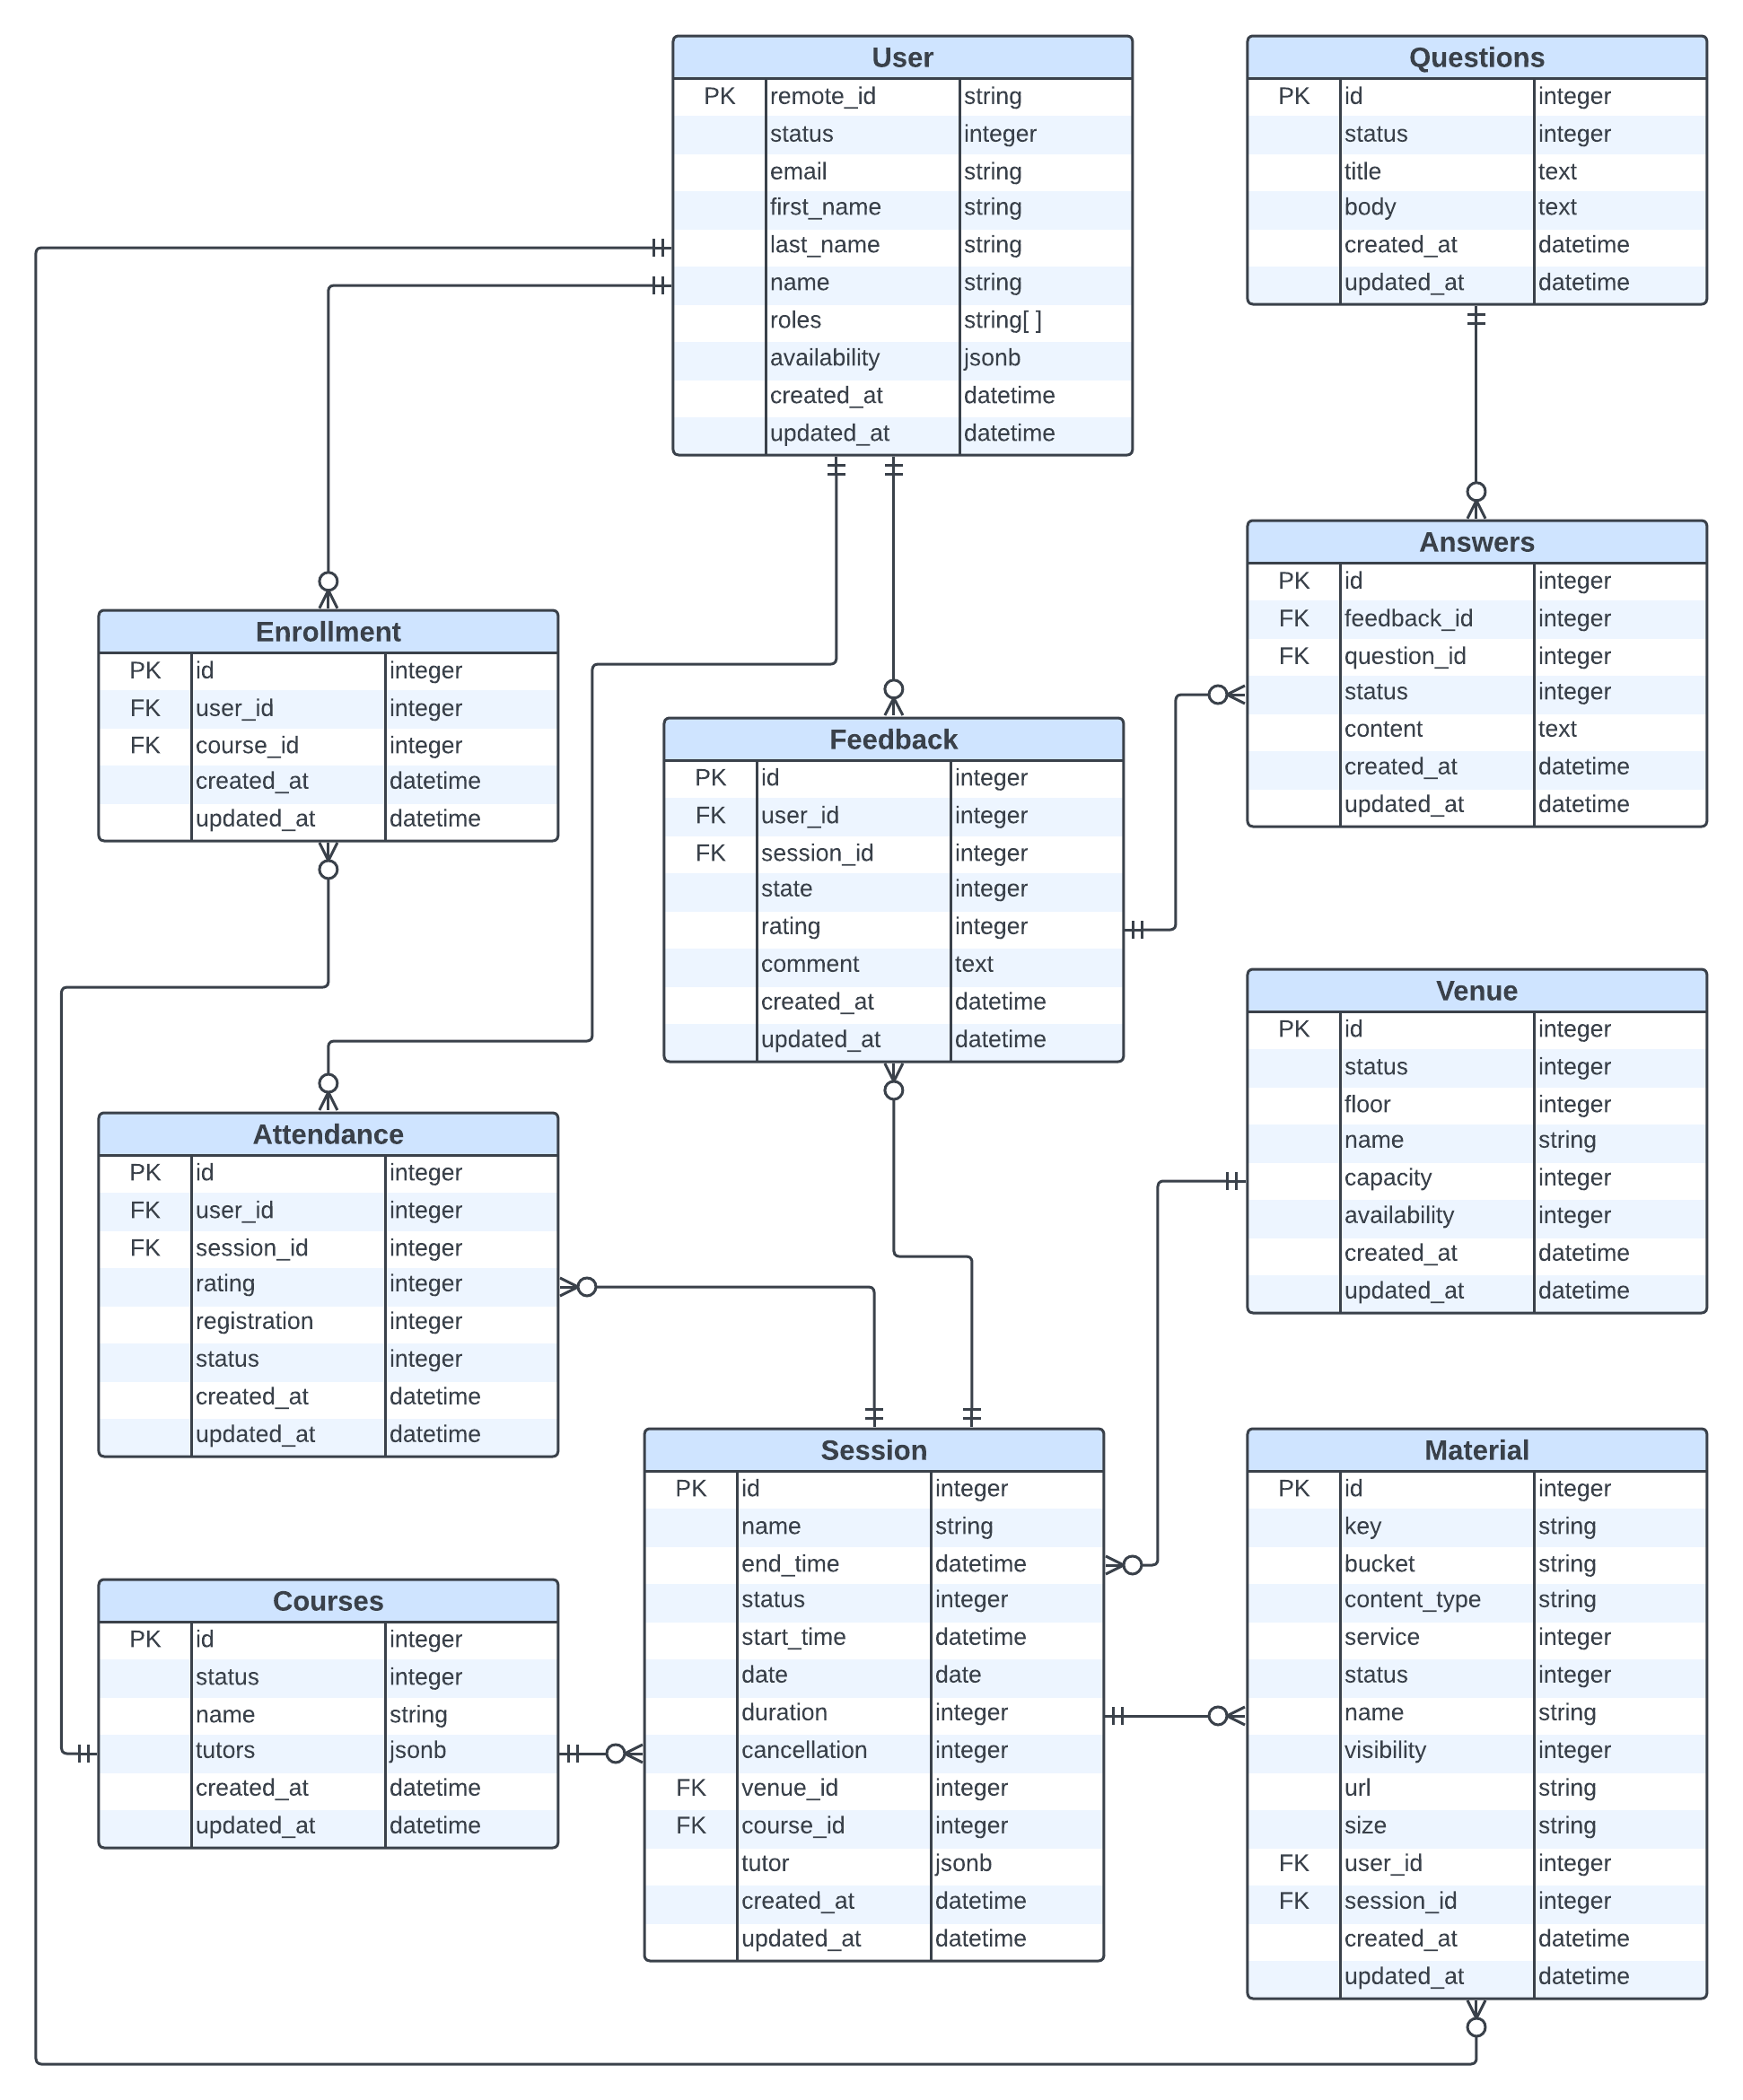
\includegraphics[width=150mm,scale=1]{figures/analysis_and_design/design/3. Physical Enitiy Attribute Relationship Diagram V2.png}}
    \caption{Database -- physical entity attribute relationship diagram}
    \label{physicalEARD}
    \end{figure}

\end{justify}


\clearpage